% !TeX encoding = UTF-8
% !TeX program  = xelatex

\documentclass[12pt,a4paper,openany]{book} 
\usepackage[typeblock=golden]{stb-titlepage}   
\usepackage[hidelinks]{hyperref}
\usepackage{parskip}
\usepackage{subcaption}
\usepackage{tabularx}
\usepackage[pdftex]{hyperref}
\usepackage{enumitem} % for compact lists
\usepackage{pdfpages}
\usepackage{threeparttable}
\usepackage{booktabs}
\usepackage{array}
\usepackage{makecell}
\usepackage{geometry}
\usepackage{hyperref}
\usepackage[title,titletoc]{appendix}
\geometry{margin=1in}
\usepackage{float}
\usepackage{graphicx}
\usepackage{subcaption}  % Add this to your preamble
\usepackage{svg}        % for \includesvg
\usepackage{pdflscape}  % for landscape pages
\usepackage{array,tabularx} % needed for \newcolumntype, tabularx
% (optional if your svgs live in figs/)
\svgpath{{figs/}}
\usepackage[round,authoryear]{natbib}
\let\cite\citep % makes \cite{...} behave like \citep{...}
\hypersetup{
	colorlinks=true,
	linkcolor=blue,
	filecolor=magenta,      
	urlcolor=black,
	citecolor=black,
	pdftitle={Your Report Title},
	pdfauthor={Your Name}
}

\makeatletter
\def\chapter{\@startsection{chapter}{0}{\z@}%
	{-3.5ex \@plus -1ex \@minus -.2ex}%
	{6ex \@plus.2ex}%
	{\normalfont\huge\bfseries}}
\makeatother



%==== Math setup =====================================================
\usepackage{amsmath}%............................. Advanced math (before fonts)
%\usepackage{amssymb}%............................ AMS Symbol fonts
\usepackage[version=4]{mhchem}
\usepackage{siunitx}           % For correct units (μmol m⁻² s⁻¹)

%==== Font setup =====================================================
\usepackage{iftex}
\ifxetex
    \usepackage[math-style=TeX,
                bold-style=TeX,
               ]{unicode-math}
    \setmainfont{Cambria}%........................ Unicode fonts  (Win)                
    \setsansfont[Scale=MatchLowercase]{Calibri}
    \setmonofont[Scale=MatchLowercase]{Consolas}
    \setmathfont{Cambria Math}
    \defaultfontfeatures{Ligatures=TeX}
    \let\bm\symbfit
\else
    \usepackage[utf8]{inputenc}%.................. Unicode file format
    \usepackage{textcomp}%........................ Additional text symbols
    \usepackage[T1]{fontenc}%..................... Type 1 outline fonts
    \usepackage{bm}%.............................. Bold math fonts
\fi
\normalfont

%==== Units and numbers ==============================================
\usepackage{siunitx}%............................. Unit, number and angle output
    \sisetup{detect-all = true, detect-family = true}
    \sisetup{output-decimal-marker = {.} ,
             group-separator = {\,},
             number-unit-product = {\,},
             inter-unit-product = \mathord{\cdot},
             exponent-product = \mathord{\times},
             separate-uncertainty = true}
         
%==== Ref's, Bib's and Nomencl =======================================
\usepackage{stb-nomencl}%......................... List of symbols 
    \renewcommand*{\UnitLabel}[1]{~[\,\unit{#1}\,]}
\usepackage{stb-bib}%............................. Bibliography (natbib internally)
    \bibliographystyle{stb-bib-eng-a}
    \renewcommand\bibfont{\small}
    %\renewcommand\bibsection{\chapter{\bibname}}

%==== Tables + Graphics + Color =====================================
\usepackage{array}%............................... Extended table defs 
    \setlength{\extrarowheight}{2pt}
\usepackage{longtable}%........................... Tables can break over pages
\usepackage{graphicx}%............................ Included graphics
\usepackage[font=small]{caption}%................. Customize captions  
\usepackage[table]{xcolor}%....................... Color setup + colortbl 
    
%==== Extra defs for template ========================================
\makeatletter
%---- TOC entries and case
    \renewcommand\contentsname{Table of contents}
    \renewcommand\listfigurename{List of figures}
    \renewcommand\listtablename{List of tables}
    \renewcommand\bibname{List of references}
    
    \renewcommand\tableofcontents{\chapter*{\contentsname}\@starttoc{toc}}
    \renewcommand\listoffigures{\chapter{\listfigurename}\@starttoc{lof}}
    \renewcommand\listoftables{\chapter{\listtablename}\@starttoc{lot}}

%---- Plagiarism signatures
    \newcommand\tstrut[1][4ex]{\rule{0pt}{#1}}
    \newcommand\tdots[1][5cm]{\makebox[#1]{\dotfill}}

%---- Summary head line
    \newcommand\sumheading{%
        \rowcolor[gray]{.9}%
        \centering\arraybackslash%
        \bfseries\normalsize}

%==== User Defs ======================================================
%
% Please insert user defined commands here
% and NOT in the document itself!
%
%
\makeatother

\let\cleardoublepage\clearpage

%==== Title Page =====================================================
\title{\textbf{Design of an Automated Electronic Greenhouse}\\[2ex]
       \large Mechatronic Project 478\\Final Report\\[2ex]}                   
\author{\Large Author: Luke Riley\\ 
        \large 23835990 \\[5ex]
        \Large Supervisor: Mrs. L Ginsburg}                
\address{Department of Mechanical and Mechatronic Engineering\\
        Stellenbosch University \\
        Private Bag X1, Matieland 7602, South Africa.}
\date{2025/07/07}                             
\Copyright{2023}{Stellenbosch University.\\ All rights reserved.}

%==== Main Document ==================================================
\setcounter{secnumdepth}{3}
\setcounter{tocdepth}{2}
\raggedbottom
\begin{document}   

\frontmatter%---------------------------------------------------------                    
\maketitle 

\include{chaps-front/chap-plagiarism}
\chapter*{AI Use Declaration}

{\setlength\labelwidth{1em}%
 \setlength\labelsep{5pt}%
 \setlength\itemindent{0pt}%
 \setlength\leftmargini{\labelwidth}%
 \setlength\topsep{0pt}%
 \setlength\partopsep{0pt}%
\begin{enumerate}
    \setlength\itemsep{\smallskipamount}%
    \setlength\parskip{0pt}%
    \small
    
    \item I am convinced and can support my claim that my assessment product is an indication of my own learning, knowledge, skills, and understanding.
    
    \item Where I have used AI tools for enhancing my own creation of ideas and words, I acknowledge that I have to declare it.
    
    \item Where I have used AI tools for generating new ideas, words, code, image-prompts for other AI Image-generating tools, or structure and even presentations (or other AI tools that can be used as assistants to the knowledge building and representing process), I have declared and documented the use of such tools and I am prepared to talk about the process I used and what it contributed to my learning and insights.
    
    \item I am aware that the lecturer can ask me to demonstrate my learning, for example through explaining the choices I made in terms of approach, content used, literature selected, conclusions drawn, etc. through an additional assessment like an oral (for example).
    
    \item I understand that if I am not able to agree to the above points, there is a chance that my academic behaviour will be deemed unethical and might lead to a disciplinary case being brought against me on the grounds of cheating or plagiarism and that the standard procedures for such behaviour will be followed.
    
    \item As per the Disciplinary Code of SU (par. 10.2.1 and 10.2.2), I understand that I take responsibility for the integrity of my work, which includes the obligation to ask for clarification from an academic member of staff if I am unsure of anything, and that I strictly adhered to all instructions received in the course of the academic assessment by relevant and authorized staff (whether the instruction is in oral or written format).
    
    \item I understand that when I am not able to document and declare my use of AI tools, this behaviour will be deemed as cheating in examinations and assessments (Disciplinary Code 1.1 c.) as I referred to “unauthorized notes, books, electronic devices or other reference material”.
\end{enumerate}}
\vspace{10mm}

\noindent
\begin{tabular}{@{}lllll@{}}
	\tstrut Signature: & \makebox[4cm]{
\includegraphics[height=1cm]{figs/sign.png}\dotfill} & & \\
	\tstrut Name: & \makebox[4cm][l]{Luke Riley\dotfill} & Student No: & \makebox[3cm][l]{23835990\dotfill} \\
	\tstrut Date: & \makebox[4cm][l]{\today\dotfill} & & \\
\end{tabular}

\chapter*{Executive summary}

\noindent
\begin{longtable}{|p{\dimexpr \linewidth-2\tabcolsep-2\arrayrulewidth}|}
\hline%------------------------------------------------------------
\sumheading  Title of Project \\
\hline%------------------------------------------------------------
 The Design of an Automated, Solar-Powered Greenhouse for Optimal Plant Growth \\[1ex]

\hline%------------------------------------------------------------
\sumheading  Objectives \\
\hline%------------------------------------------------------------
 Design and build a small-scale greenhouse capable of automating all the necessary elements to sustain amicable living conditions for various plants while enabling the user with wireless monitoring capabilities. \\[1ex]

\hline%------------------------------------------------------------
\sumheading  What is current practice and what are its limitations? \\
\hline%------------------------------------------------------------
 Current domestically applicable greenhouses rely heavily on active monitoring and care, this requires significant labour and time and can still not achieve ideal living conditions for some plants.  \\[1ex]

\hline%------------------------------------------------------------
\sumheading  What is new in this project? \\
\hline%------------------------------------------------------------
This project introduces a system capable of wirelessly monitoring multiple parameters within the greenhouse, including temperature, humidity, soil moisture, air composition, and airflow, and enables effective control of these parameters within user-defined ranges. The integration of solar power helps to offset the system’s energy requirements, reinforcing its sustainability. \\[1ex]

\hline%------------------------------------------------------------
\sumheading  If the project is successful, how will it make a difference? \\
\hline%------------------------------------------------------------
 It will introduce the ease of automation to domestic greenhouses, demystifying the struggles of home farming while encouraging self-sufficiency. By promoting food independence, it can reduce reliance on the national food supply chain, empowering individuals and communities to grow their own fresh produce sustainably.\\[1ex]

\hline%------------------------------------------------------------
\sumheading  What are the risks to the project being a success? Why is it expected to be successful? \\
\hline%------------------------------------------------------------
 The system may not be efficient enough at controlling the desired parameters. There may be delays due to time management issues. However, through thorough research, modular design and allowing buffer periods for unexpected delays, the project shouldn’t be able to fail. \\[1ex]

\hline%------------------------------------------------------------
\sumheading  What contributions have/will other students made/make? \\
\hline%------------------------------------------------------------
 No other students have/ will contribute to this design. \\[1ex]

\hline%------------------------------------------------------------
\sumheading  Which aspects of the project will carry on after completion and why? \\
\hline%------------------------------------------------------------
 Further research on the economic feasibility of the project may be conducted.  \\[1ex]

\hline%------------------------------------------------------------
\sumheading  What arrangements have been/will be made to expedite continuation? \\
\hline%------------------------------------------------------------
  Thorough documentation of the design process will allow for continuation or improvements to be made. Modular design should allow for ease of maintenance as well as allow for the upgrading of any components if necessary.  \\[1ex]

\hline%------------------------------------------------------------
\end{longtable}


\chapter*{Acknowledgements}

\begin{center} I would like to begin by sincerely thanking my supervisor for proposing a project that I feel deeply passionate about, and for providing the guidance and support that allowed it to grow into what it has become. I also wish to acknowledge all the staff in the M\&M Engineering Department at Stellenbosch University who assisted in many aspects of the project. In no paticular order: Mr Cobus and Ferdi Zietsman, Mr Llewellyn Kordom, Mr Nathi HLwempu, Mr Kevin Neaves, Charl Adonis, Mrs. Paulse Simorne and Mr Cobus Samuels. This project could not have taken the shape it did without their dedication, expertise, and passion for engineering and their respective crafts.
\end{center}



\chapter*{ECSA Outcomes Self-Assessment}

\setlength{\tabcolsep}{6pt}
\renewcommand{\arraystretch}{1.15}

\begin{table}[H]
	\centering
	\begin{tabularx}{\textwidth}{|
			>{\raggedright\arraybackslash}X |
			>{\raggedright\arraybackslash}p{0.38\textwidth} |
		}
		\hline
		\textbf{ECSA Outcome} & \textbf{Addressed in Sections:} \\
		\hline
		\textbf{GA 1. Problem solving:} Demonstrate competence to identify, assess, formulate and solve convergent and divergent engineering problems creatively and innovatively.
		&
		\begin{itemize}[leftmargin=*, nosep]
			\item Concept Design Section~\ref{chap:concept}
		\end{itemize}
		\\ \hline
		
		\textbf{GA 2. Application of scientific and engineering knowledge:} Demonstrate competence to apply knowledge of mathematics, basic science and engineering sciences from first principles to solve engineering problems.
		&
		\begin{itemize}[leftmargin=*, nosep]
			\item Calculations Appendix~\ref{chap:calcs}
		\end{itemize}
		\\ \hline
		
		\textbf{GA 3. Engineering Design:} Demonstrate competence to perform creative, procedural and non-procedural design and synthesis of components, systems, engineering works, products or processes.
		&
		\begin{itemize}[leftmargin=*, nosep]
			\item Concept Design Section~\ref{chap:concept}
			\item Detailed Design Section~\ref{chap:design}
		\end{itemize}
		\\ \hline
		
		\textbf{GA 5. Engineering methods, skills and tools, including Information Technology:} Demonstrate competence to use appropriate engineering methods, skills and tools, including those based on information technology.
		&
		\begin{itemize}[leftmargin=*, nosep]
			\item Design Evaluation Section~\ref{chap:eval}
		\end{itemize}
		\\ \hline
		
		\textbf{GA 6. Professional and technical communication:} Demonstrate competence to communicate effectively, both orally and in writing, with engineering audiences and the community at large.
		&
		\begin{itemize}[leftmargin=*, nosep]
			\item Project Proposal
			\item Progress Report / Presentation
			\item Safety Report
			\item First Draft / Final Report
			\item Final Presentation
		\end{itemize}
		\\ \hline
		
		\textbf{GA 8. Individual, Team and Multidisciplinary Working:} Demonstrate competence to work effectively as an individual, in teams and in multi-disciplinary environments.
		&
		\begin{itemize}[leftmargin=*, nosep]
			\item Safety Report Section~\ref{chap:safety}
			\item Provided Equipment Section~\ref{sec:provided}
		\end{itemize}
		\\ \hline
		
		\textbf{GA 9. Independent Learning Ability:} Demonstrate competence to engage in independent learning through well-developed learning skills.
		&
		\begin{itemize}[leftmargin=*, nosep]
			\item Literature Review and Market Research Section~\ref{chap:lit}
			\item Detailed Design Section~\ref{chap:design}
		\end{itemize}
		\\ \hline
	\end{tabularx}
	\caption{ECSA Graduate Attributes Mapping}
	\label{tab:ecsa_outcomes}
\end{table}




% Use \chapter*{} before TOC
\hypersetup{
	linkcolor=black,
	citecolor=black,
}
\tableofcontents

% Use \chapter{} after TOC

\listoffigures
\listoftables
\hypersetup{
	linkcolor=blue,
	citecolor=black,
}
\chapter{List of symbols}
% Use stb-nomenclature + siunitx

\begin{Nomencl}[1cm]
\NomGroup{Constants}%-----------------------------------------------
   

\NomGroup{Variables}%-----------------------------------------------
   
  
    \item[$I$]  \UnitLine{Moment of Inertia              }{kgm^2}
    \item[$E$]  \UnitLine{Youngs Modulus             }{Pa}
    \item[$v$]  \UnitLine{Poisons Ratio             }{}
    \item[$P$]  \UnitLine{Dynamic Pressure           }{Pa}
    \item[$D$]  \UnitLine{Flexural Rigidity           }{Nm}
    \item[$p$]  \UnitLine{Density          }{kg/m^3}\\

\NomGroup{Vectors and Tensors}%-------------------------------------
    \item[$\overrightarrow{\bm{v}}$] Velocity

\NomGroup{Subscripts}%----------------------------------------------
    \item[$\mathrm{h}$] Height
    \item[$t$]          Thickness
    \item[$l$]          Length
    \item[$b$]          Breadth
    \item[$v$]          Velocity

\end{Nomencl}

\begin{Nomencl}[1cm]
\NomGroup{Abreviations}%-----------------------------------------------
    \item[ppm] parts per million
    \item[PAR] Photosynthetic Active Radiation
    \item[PPFD] Photosynthetic Photon Flux Density
    \item[DLI] Daily Light Integral
    \item[VWC] Volumetric Water Content
    \item[HVAC] Heating Ventilation Air Conditioning
    \item[CO2] Carbon Dioxide
    \item[IoT] Internet of Things
    \item[IDE] Integrated Developement Environment
    \item[TCP] Transmission Control Protocol
    \item[IP] Internet Protocol
    \item[PV] Photo Voltaic
    \item[DC] Direct Current
    \item[AC] Alternating Current
    \item[MPPT] Maximum Power Point Tracking
    \item[RH] Relative Humidity
    \item[GPIO] Generel Purpose Input Output
    

\end{Nomencl}


\mainmatter%----------------------------------------------------------
\numberwithin{figure}{chapter}
\numberwithin{table}{chapter}

\chapter{Introduction}

\section{Background}
As food insecurity increases and available farmland decreases due to deforestation and urbanization \citep{Olagunju2015}, small-scale greenhouses offer a practical way to grow food in limited spaces. Greenhouses help protect crops from harsh weather and allow for better control of growing conditions, which can improve yield, product quality and lengthen market availability \citep{vox}. By using transparent materials to trap heat and light, they create a more stable environment for plants. However, maintaining this environment can be labour intensive and often requires regular monitoring to manage temperature, humidity, and watering.

\section{Objectives}

\begin{itemize}
    \item Design a small-scale greenhouse that can monitor and adjust key environmental factors such as temperature, soil moisture, and humidity.
    \item Allow users to input and control target conditions based on the specific requirements of different plant types.
    \item Integrate a solar power system to enable off-grid operation.
    \item Address limitations in simultaneous parameter control by prioritizing adjustments that best support overall plant health.
    \item Test and evaluate the performance of the greenhouse system to assess its effectiveness and reliability in maintaining suitable growing conditions.
\end{itemize}

\section{Motivation}

Greenhouses provide ideal growing conditions but require constant monitoring and adjustments, making them labour-intensive and inaccessible for many. By reducing manual effort and enabling customization for different plants, this project aims to empower users to grow food efficiently and sustainably with minimal effort. Additionally, the off-grid solar design promotes energy independence and environmental sustainability, aligning with global efforts to combat food insecurity and climate change. This project bridges technology and agriculture, making greenhouse farming accessible, efficient, and eco-friendly.

\section{Methodology}

This project adopts the engineering design methodology outlined by Dieter and Schmidt, providing a structured framework to guide the development of the electronic greenhouse. \citep{Dieter} This methodology encompasses several key phases:

\begin{enumerate}
    \item \textbf{Problem Definition and Need Identification:} This initial phase emphasizes understanding the problem's scope and identifying the specific needs the design aims to fulfill.
    
    \item \textbf{Concept Generation:} Developing multiple design concepts that address the identified needs and constraints. Multiple potential solutions are brainstormed without immediate judgment, encouraging a broad exploration of ideas.
    
    \item \textbf{Concept Selection:} Here, the various concepts are evaluated against predefined criteria to select the most promising solution.
    
    \item \textbf{Detailed Design:} Precise specifications for all components are established, including materials, dimensions, and tolerances, preparing the design for manufacturing.
    
    \item \textbf{Design Evaluation:} Testing the designed system to determine its functionality and performance.
\end{enumerate} By following this systematic approach, the project ensures a thorough exploration of design alternatives and a robust development process for the electronic greenhouse.
\chapter{Literature review and market research}\label{chap:lit}

\section{Environmental Requirements for Optimal Plant Growth }

Different plant species require a careful balance of light, temperature, humidity, and water supply to achieve optimal growth. The following sections outline the key environmental parameters that must be monitored and controlled to create ideal growing conditions within the greenhouse.

\subsection{Temperature} 

Plants regulate transpiration and cooling through specialized organs known as stomata located on the surface of leaves. These pores can open or close to control the release of water vapor, helping the plant manage water loss and internal temperature \cite{xu2024_high_temp_stomatal}. As ambient temperatures rise, open stomata allow for increased evaporation, aiding in the cooling process. However, excessive heat can lead to excessive water loss and stress. While optimal temperature ranges vary depending on the plant species and its growth stage, greenhouse temperatures are generally best maintained between \SI{15}{\degreeCelsius} and \SI{30}{\degreeCelsius} to support healthy plant development \cite{kosan2020}.

\subsection{Light} 

Light indirectly influences water loss in plants by triggering the opening of stomata, which enables gas exchange and \ce{CO2} uptake for photosynthesis \cite{kochetova2022}. However, excess light can cause overheating and increased transpiration, so it must be carefully managed along with temperature. Some plants are sensitive to photoperiodism, meaning their flowering depends on day length. In greenhouses, adjusting light exposure can control flowering times, allowing for year-round yield \cite{greenhouse_lighting}.

To evaluate light conditions within greenhouses, specific terminology and measurement units are used to describe both the quantity and quality of light that plants receive. The spectrum of light between 400 and 700~nanometres (nm) is recognized as \textbf{photosynthetically active radiation (PAR)}, the range most efficiently used by plants for photosynthesis \citep{sena2024}. Monitoring this specific light range is essential for optimizing plant productivity.

A key metric within the PAR range is the \textbf{photosynthetic photon flux density (PPFD)}. PPFD refers to the number of photons, within the PAR spectrum, that strike a square meter of plant surface each second. It is expressed in micromoles per square meter per second (\si{\micro\mole\per\metre\squared\per\second}). PPFD measurements help determine if the lighting levels in the greenhouse are sufficient to support healthy plant growth. Insufficient PPFD may lead to slow growth or poor productivity due to inadequate light. Excessively high PPFD can result in photoinhibition or physical damage to plant tissues \citep{measuring_ppfd}.

To relate PPFD to the more commonly used unit of \textit{lux}, an approximate conversion can be applied 
The exact factor depends on the spectrum of the light source, but for white LEDs, a typical approximation is:  

\begin{equation}
	\text{PPFD} \; (\si{\micro\mole\per\metre\squared\per\second}) 
	\;\approx\; \frac{\text{Illuminance (lux)}}{54} \label{ppfd}
\end{equation}

where 1~\si{\micro\mole\per\metre\squared\per\second} corresponds to roughly 54~lux. 
This relationship allows lux sensor readings to be interpreted in terms of usable light for photosynthesis.  \citep{ahn2017} Ideal PPFD ranges for Seedlings range from 100–300, while vegatative range from 300–600 \si{\micro\mole\per\metre\squared\per\second} \citep{definitiveGrowLight2024}. Monitoring and balancing light intensity through artificial lighting systems and proper greenhouse design is therefore essential to maintain optimal photosynthetic activity without causing plant stress.


\subsection{Humidity} 

Humidity plays a critical role in plant health by influencing the rate of transpiration, the process through which plants absorb water and nutrients from the soil and release water vapor through stomata. In high humidity environments, the air becomes too saturated with moisture, which suppresses transpiration. This reduction in water and nutrient uptake can hinder plant growth and development.

Conversely, in low humidity conditions, transpiration rates can become excessively high due to the dry air. In response, plants often close their stomata to conserve water, but this also limits gas exchange and light absorption, leading to water stress and reduced growth \cite{nederhoff}.

To support optimal development, research indicates that the ideal relative humidity (RH) range for most greenhouse crops lies between 30\% and 90\%. Maintaining this balance helps prevent both under- and over-transpiration, ensuring steady nutrient uptake and healthy physiological function \cite{pepper_guide}.



\subsection{Carbon Dioxide} 

For most greenhouse crops, net photosynthesis increases significantly as \ce{CO2} concentrations rise from ambient levels (approximately 340~ppm) up to around 1,000~ppm, potentially boosting photosynthesis by up to 50\%. However, the benefit of \ce{CO2} supplementation varies by crop and may not be economically justifiable under low light conditions or for certain species like tulips and Easter lilies, which show little response \cite{carbon_dioxide_enrichment}.

\ce{CO2} enters plants through stomata via diffusion, and its uptake is influenced by external \ce{CO2} concentration as well as factors such as light, temperature, humidity, and water availability. While plants generally grow well at ambient \ce{CO2} levels, concentrations can drop to as low as 200~ppm in sealed greenhouses during the day due to plant uptake. This drop can significantly reduce photosynthesis, sometimes with an effect comparable to the enhancement achieved by raising \ce{CO2} levels to 1,300~ppm.


\begin{figure}[h]
	\centering
	\fbox{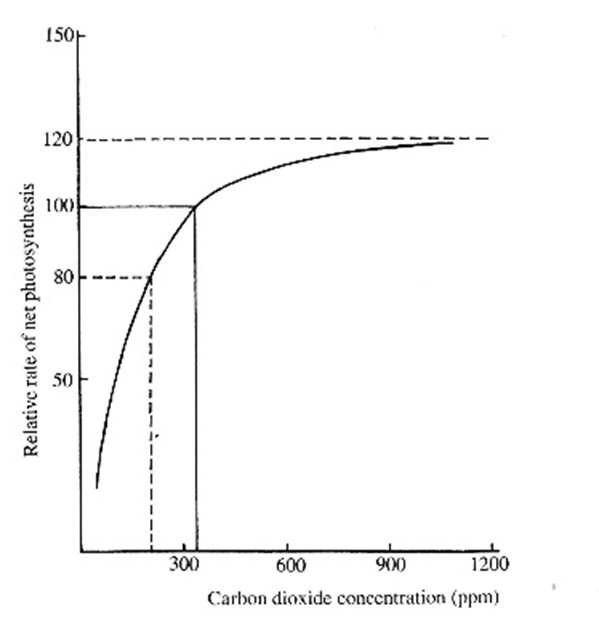
\includegraphics[width=0.55\textwidth]{figs/Co2.jpg}}
	\caption{Effect of \ce{CO2} concentration on photosynthesis rate. \cite{carbon_dioxide_enrichment}. }
	\label{fig:photosynthesis}
\end{figure}

As seen in the figure \ref{fig:photosynthesis}, at low \ce{CO2} concentrations (below approximately 300~ppm), the rate of photosynthesis increases sharply as \ce{CO2} concentration rises. However, beyond approximately 400--500~ppm (close to ambient fresh air levels), further increases in \ce{CO2} concentration have little to no additional effect on the photosynthesis rate, as the curve begins to plateau. Therefore, monitoring and maintaining ambient \ce{CO2} concentrations through simple ventilation can be sufficient to support healthy plant growth, without the need for costly \ce{CO2} enrichment.

\subsection{Water} 

A continuous supply of high-quality water is essential for plant transpiration, a process that not only cools the leaves but also facilitates the transport of nutrients from the roots to the leaves and fruits \cite{olabisi2022}.

To monitor soil moisture effectively, \textbf{Volumetric Water Content (VWC)} is commonly used. VWC is expressed as a percentage and represents the volume of water present in a given volume of soil.

\begin{equation}
\text{VWC (\%)} = \frac{\text{Volume of Water}~(\mathrm{cm}^3)}{\text{Volume of Soil}~(\mathrm{cm}^3)} \times 100
\end{equation}

This measurable metric provides valuable information for irrigation management, ensuring that plants receive adequate moisture for optimal growth without the risk of overwatering or water stress.


\section{Structural Design Standards}

\subsection{Achitecture of a greenhouse}\label{architecture}

Beyond structural integrity, the architectural design of the greenhouse plays a key role in regulating its internal climate. Greenhouses function either to retain heat during cold periods or to exclude heat in hotter seasons, with the aim of maintaining a productive microclimate for plant growth \cite{ghani2019}. In South Africa’s hot summers, a primary design consideration is minimizing heat buildup, making passive and active cooling essential.

One of the most influential architectural elements is the shape of the greenhouse, particularly the roof profile. The geometry directly affects solar irradiance levels inside the structure. In hot, arid environments, the optimal greenhouse form is one that minimizes solar gain during summer while maximizing it in winter, thereby supporting year-round cultivation. Research has shown that the roof angle and shape significantly influence the amount and distribution of solar radiation received \cite{ghani2019}.

A well-designed greenhouse structure must therefore strike a balance between mechanical resilience (to environmental loads) and thermal efficiency (to manage light and heat), with the shape and orientation of the building serving both functions. There are generally 4 main shapes discussed:

\begin{figure}[h]
    \centering
    \fbox{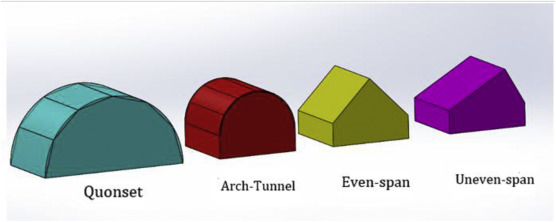
\includegraphics[width=0.8\textwidth]{figs/shapes.jpg}}
    \caption{Main Greenhouse Shapes. \cite{Sethi2009}. }
    \label{fig:photosynthesis}
\end{figure}

Choosing the right shape involves balancing structural load requirements with climate control goals, and often depends on regional weather patterns, crop types, and energy availability.

In terms of geographic suitability, greenhouse performance varies significantly with latitude and shape. For example, at \SI{31}{\degree}N latitude, even-span and Quonset greenhouses tend to receive more solar radiation in winter and less in summer, which is ideal for regions with significant seasonal temperature variation. However, at higher latitudes such as \SI{50}{\degree}N, uneven-span greenhouses are more effective for maintaining suitable internal conditions throughout the year.
\citep{Sethi2009}

The inclination angle significantly affects solar heat gain by altering the amount of radiation absorbed by the greenhouse surface. \citep{Mellalou2022}. As shown in figure \ref{fig:inclin} below, solar energy gaining rates decrease with steeper roof angles such as the \SI{27}{\degree} inclination angle seen below. While both N--S and E--W orientations perform similarly at \SI{12}{\degree} inclination, the E--W orientation consistently captures more energy at higher inclinations. This highlights the importance of optimizing both greenhouse orientation and tilt to balance heat gain and internal climate control.

\begin{figure}[h]
    \centering
    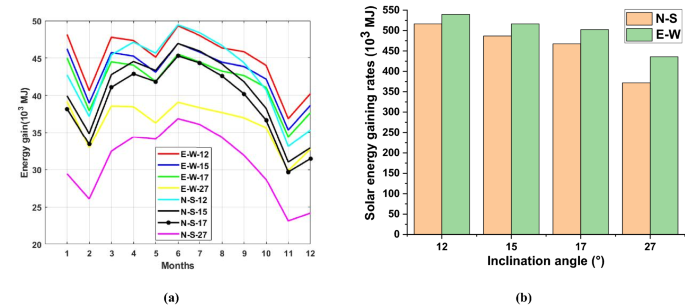
\includegraphics[width=0.95\textwidth]{figs/inclination.png}
    \caption{Solar radiation gain vs inclination angles \citep{Mellalou2022}. }
    \label{fig:inclin}
\end{figure}

\subsection{Sawtooth Design}

The sawtooth greenhouse has gained popularity in tropical and subtropical climates due to its unique roof design and natural ventilation system. This roof features several curved, sawtooth-shaped sections, with vertical windows at the highest points to enhance natural ventilation. It uses natural resources like airflow and gravity to regulate the temperature and humidity inside the greenhouse, reducing reliance on external energy sources such as electricity \citep{inson_greenhouse}. Compared to traditional greenhouses, sawtooth greenhouses provide better ventilation, temperature control, and structural stability, making them ideal for hot, humid regions. As the temperature inside the greenhouse rises, warm air naturally ascends and exits through the vertical windows at the top, while cooler air enters from below, creating a natural airflow cycle. The vertical windows are often controlled by a roll-up mechanism that opens for ventilation and closes for insulation when needed.

\begin{figure}[H]
    \centering
    \fbox{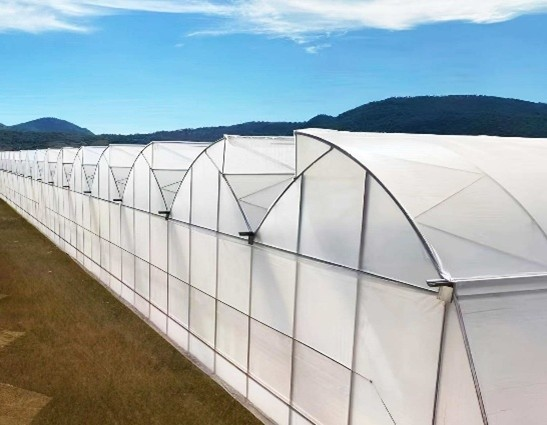
\includegraphics[width=0.45\textwidth]{figs/sawtooth.jpg}}
    \caption{Sawtooth Greenhouses \citep{inson_greenhouse}. }
    \label{fig:photosynthesis}
\end{figure}

\subsection{Construction techniques}

Greenhouses are classified by structure (wooden-, pipe-, and truss-framed) and by framing material. Wooden frames suit small, simple builds; pipe/steel frames add strength for larger spans; and truss systems deliver maximum rigidity for big installations. Materials are chosen for cost, durability, and maintenance: wood is cheap and accessible, however aluminium offers the best mix of strength, corrosion resistance, and low upkeep thus often the long-term choice \citep{dalai2020}.

\subsection{Covering materials}\label{cover}

The choice of covering material greatly influences the internal environment, light transmission, durability, and cost of a greenhouse. The most used materials include glass, plastic film, and rigid panels.

\textbf{Glass Greenhouses:} Glass offers high light transmission, good air circulation, and lower internal humidity, which helps reduce disease incidence. However, they are more expensive to build and maintain compared to plastic-covered structures. They introduce additional maintenance challenges and potential issues due to glass's fragile nature.

\textbf{Plastic Film Greenhouses:} Covered with flexible materials such as polyethylene, polyvinyl chloride, or polyester, plastic film greenhouses are cost-effective and require less heating. Their main disadvantage is a shorter lifespan, even UV-stabilized films typically last no more than 4 years.

\textbf{Rigid Panel Greenhouses:} Made from polycarbonate, fiberglass-reinforced plastic, acrylic, or PVC rigid panels, these coverings offer better durability (up to 20 years) and more uniform light distribution. However, the panels are prone to collecting dust and algae, which reduces light transmission over time \citep{verma2022}.

\section{Enviromental control}

Automated control of environmental parameters such as irrigation, heating and cooling, humidity, and airflow reduces manual workload and contributes to improved plant health. The following sections outline key industry standards and practices for managing these environmental factors effectively.

\subsection{Irrigation Systems}\label{irrig}

The right water system is key to the success of any greenhouse system. As greenhouse plants have a limited soil buffer, precision irrigation systems are vital to ensure high-quality crops and yields \citep{vegtech_netafim}.
Some of the most used types of irrigation include:

\textbf{Drip Irrigation:} This system delivers water directly to the base of each plant through a network of tubes and emitters, ensuring precise watering and minimizing water waste. By keeping foliage dry, it reduces the risk of fungal diseases. Drip irrigation is highly efficient and can be automated for consistent application \citep{cedar_greenhouse}.

\textbf{Misting System:} Misting systems distribute fine water droplets from above to hydrate plants and maintain humidity within the greenhouse. It provides broad and uniform coverage suitable for various crops, particularly delicate seedlings and humidity-loving plants. While effective for moisture control, excessive use can wet plant foliage, potentially elevating the risk of disease. Proper management is essential to mitigate these concerns.

\textbf{Ebb and Flow Systems:} Also known as flood and drain systems, ebb and flow setups periodically flood the growing area with nutrient-rich water and then allow it to drain away. This cyclical process ensures that plant roots receive adequate moisture and nutrients while preventing waterlogging. Ebb and flow systems are commonly used in hydroponic greenhouse operations \citep{floraflex_irrigation}. However, these systems require complex hydraulic components and precise nutrient management, increasing system complexity and maintenance requirements.

\subsection{Heating and Cooling Systems} \label{heat}

Efficient greenhouse climate control uses \textbf{passive} and \textbf{active} methods \citep{vegtech_netafim}. Passive approaches rely on natural processes and strategic design, needing no external energy; active systems use mechanical/electrical equipment requiring external energy inputs. 

\subsubsection*{Passive Heating}
This approach leverages solar energy to naturally warm the greenhouse. By incorporating design elements such as proper orientation, insulation, and thermal mass (e.g., water barrels or rock walls), heat is absorbed during the day and released at night, maintaining a stable internal temperature \citep{kumari2007}.

\subsubsection*{Active Heating}
To compensate for temperature drops, especially during winter nights, various heating systems are utilized. Options include unit heaters such as electric fan heaters, gas heating systems, heat lamps, and solar heating systems. The choice of system depends on factors such as greenhouse size, crop requirements, and energy efficiency considerations.

\subsubsection*{Passive Cooling}
Natural ventilation is employed to facilitate air exchange between the interior and exterior, helping to dissipate excess heat. This can be achieved through operable vents in the roof and sidewalls, allowing warm air to escape and cooler air to enter \citep{faridi_cooling}.

\subsubsection*{Active Cooling}
In situations where passive cooling is insufficient, active methods like evaporative cooling are implemented. This technique involves using fans and wet pads to cool the air through water evaporation, effectively reducing internal temperatures even during hot periods \citep{verma_cooling}. Integrating both passive and active systems allows for a comprehensive approach to climate control in greenhouses, ensuring optimal growing conditions across varying external temperatures and weather conditions.

\subsection{Humidity Control}

A cost-effective way to achieve humidity control in a controlled environment involves a misting system that sprays mist over the entire crop, thereby increasing humidity~\citep{controlling_humidity}. It is essential to recognize that relative humidity is strongly influenced by temperature: warm air can hold more moisture than cooler air. As temperatures drop, the relative humidity increases, even if the actual amount of water vapor in the air remains constant. \citep{Lawrence2005RHdewpoint}

Traditional humidity control methods often involve a combination of heating and ventilation. When humidity exceeds the desired level, greenhouse vents and windows can be opened to expel warm, moist air and allow cooler, drier air to enter. While this effectively reduces humidity, it can also result in unwanted heat loss. As a result, additional heating may be required to maintain optimal growing temperatures. Achieving a balance between ventilation and heating is therefore essential for stable humidity and temperature regulation within the greenhouse environment~\citep{pepper_guide}.

\subsection{Airflow}

\subsubsection*{Airflow in Greenhouse Environments}

Effective airflow is crucial in greenhouse environments to maintain optimal growing conditions and prevent plant diseases. Proper air movement helps disperse microclimates, preventing localized areas of trapped moisture, and ensures uniform temperature and humidity levels throughout the greenhouse. This uniformity is vital for consistent plant growth and reducing the risk of fungal infections~\citep{pepper_guide}.

\subsubsection*{Airflow Components in Greenhouses}

\begin{itemize}
    \item \textbf{Roof Vents:} These allow hot air to escape from the top of the greenhouse, facilitating natural convection. As warm air rises and exits, cooler air is drawn in, aiding in temperature regulation.

    \item \textbf{Side Vents:} Positioned along the sides, these vents promote cross-ventilation by enabling fresh air to flow horizontally through the structure. This movement helps maintain consistent temperature and humidity levels.

    \item \textbf{Intake and Exhaust Fans:} Mechanical systems that actively move air in and out of the greenhouse. Intake fans draw in fresh, usually cooler air, while exhaust fans expel stale, humid air, preventing the buildup of moisture and heat~\citep{airflow_growersnetwork}.

    \item \textbf{Horizontal Airflow (HAF) Fans:} These fans circulate air horizontally within the greenhouse, ensuring even distribution of temperature and humidity. By moving air consistently, HAF fans help eliminate microclimates and reduce condensation on plant surfaces, thereby lowering the risk of disease~\citep{lopez2013}.
\end{itemize}

\begin{figure}[h]
    \centering
    \begin{subfigure}[b]{0.45\textwidth}
        \centering
        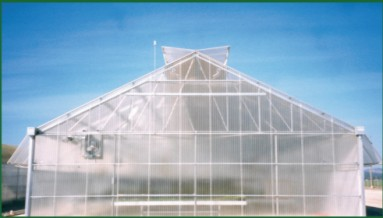
\includegraphics[width=\textwidth]{figs/airflow1.jpg}
        \caption{Greenhouse profile}
        \label{fig:image1}
    \end{subfigure}
    \hfill
    \begin{subfigure}[b]{0.45\textwidth}
        \centering
        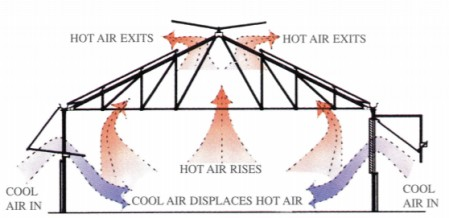
\includegraphics[width=\textwidth]{figs/airflow2.jpg}
        \caption{Ventilation airflow}
        \label{fig:image2}
    \end{subfigure}
    \caption{Airflow \citep{airflow_growersnetwork}}
    \label{fig:side_by_side}
\end{figure}

The figures above show an active ventilation system displaying the use of side and roof vents to promote healthy air circulation and thermal control. Integrating these components effectively creates a balanced airflow system that supports healthy plant development by regulating environmental conditions and minimizing disease-promoting factors.

\subsection{Automation and Environmental Control}

Automation in greenhouses allows for precise control of environmental conditions such as temperature, humidity, light, and \ce{CO2}. Using sensors and controllers, these systems enhance efficiency, minimize manual labor, and support consistent crop development. Depending on the greenhouse's complexity, control systems can range from simple microcontrollers to advanced PLCs and IoT-based architectures \citep{farooq2022}.

\subsubsection{Sensors}

\begin{itemize}
  \item \textbf{Temperature Sensors}: Monitor the internal temperature of the greenhouse.\\
  \textit{Common types}: Thermistors, RTDs, DS18B20 (digital)
  
  \item \textbf{Humidity Sensors}: Measure the ambient humidity levels.\\
  \textit{Common types}: DHT22, SHT31

  \item \textbf{Soil Moisture Sensors}: Detect the moisture content in soil.\\
  \textit{Common types}: Capacitive soil moisture sensors, resistive sensors

  \item \textbf{Light Sensors}: Measure light intensity reaching plant surfaces.\\
  \textit{Common types}: BH1750, TSL2561, TSL2591

  \item \textbf{\ce{CO2} Sensors}: Monitor carbon dioxide concentration.\\
  \textit{Common types}: MH-Z19, Senseair S8
\end{itemize}

Sensor data is fed into a controller, such as a PLC, Arduino, or Raspberry Pi, enabling automated decision-making for heating, cooling, irrigation, and other critical operations \citep{automated_greenhouse_iot}.


\subsubsection{Controllers} \label{control}

\textbf{Programmable Logic Controllers (PLC):} A Programmable Logic Controller (PLC) is a robust, industrial-grade computer used for controlling and monitoring industrial processes. It operates by receiving inputs, processing the data, and triggering outputs based on pre-programmed logic. PLCs are widely used in greenhouse automation due to their flexibility and reliability. Built with rugged designs and solid-state components, PLCs ensure long-term, reliable performance in harsh environments. The main drawback of PLCs is their higher power requirements and higher cost compared to microcontroller-based systems, which may limit their use in smaller or cost-sensitive projects \citep{dwinugroho2021greenhouse}.

\textbf{Microcontrollers:} Microcontrollers are small, programmable devices that can control a wide range of greenhouse automation tasks, such as environmental monitoring and data logging. The following microcontrollers are commonly used in greenhouse automation:

\begin{itemize}
    \item \textbf{Raspberry Pi:} A low-cost, powerful computer board frequently used in Internet of Things (IoT) applications. \citep{raspberrypi}. It offers greater processing power and versatility than simpler microcontrollers like Arduino and ESP8266. Raspberry Pi is ideal for more complex greenhouse automation systems, including advanced data collection and analysis 
    
    \item \textbf{ESP8266/ESP32:} These low-cost Wi-Fi microchips, developed by Espressif Systems, include built-in transmission control protocol (TCP/IP) stacks and microcontroller capabilities. The ESP8266 and ESP32 are widely used in IoT applications for connecting devices to the internet. They are compatible with the Arduino IDE, making them a popular choice for developing cost-effective, connected greenhouse systems \citep{esp_esp32}.
    
    \item \textbf{Arduino:} An open-source platform based on simple microcontroller chips, Arduino is designed for ease of use and flexibility. It is suitable for basic greenhouse monitoring and control tasks. Arduino's simplicity and large community make it an excellent choice for entry-level projects that require straightforward automation \citep{Yahaya2019}.
\end{itemize}

These controllers play a critical role in facilitating data logging and remote monitoring as well as enabling automated greenhouse systems to efficiently manage environmental factors such as temperature, humidity, and light for improved crop management.

\subsection{Wireless Connectivity and Actuation}

\textbf{Wireless Connection:}

ThingSpeak can be used with both Raspberry Pi and Arduino to wirelessly upload and visualize sensor data. ThingSpeak is an IoT analytics platform that allows real-time data collection, storage, and visualization from connected devices. Once connected to Wi-Fi, the Arduino or Raspberry Pi can send HTTP (Hypertext Transfer Protocol) requests to ThingSpeak's API (Application Programming Interface) to upload sensor readings. By integrating ThingSpeak with these controllers, one can effectively monitor and analyze sensor data remotely, making it a valuable tool for greenhouse automation and other IoT applications \citep{thingspeak}.

\textbf{Actuators and Switches:}

In greenhouse automation, relays are essential components that allow low-voltage control signals to switch high-voltage appliances such as irrigation pumps, lights, and ventilation systems on and off. This ensures efficient and safe operation of the system. These relays can be activated using the low voltage signals sent by the controller \citep{farooq2022}.

\section{Energy Efficiency \& Sustainability}

Solar power lets greenhouses run equipment on a clean, renewable source, cutting costs and environmental impact. Paired with batteries, it keeps systems running through outages and seasons, enabling stable, year-round crop production regardless of outside weather.

\subsection{Key Requirements for Solar System}

Incorporating a solar power system into a greenhouse requires understanding its essential components, each playing a pivotal role in energy capture, conversion, storage, and utilization. The key elements include:

\begin{enumerate}
    \item \textbf{Solar Panels (Photovoltaic Modules):} Solar panels are the primary components that capture sunlight and convert it into direct current (DC) electricity through photovoltaic cells \citep{Krisciunas2023}.
    
    \item \textbf{Inverter:} The inverter transforms the DC electricity generated by the solar panels into alternating current (AC) electricity
    
    \item \textbf{Charge Controller with Maximum Power Point Tracking (MPPT):} A charge controller manages the flow of electricity from the solar panels to the batteries, preventing overcharging and prolonging battery life. MPPT is an algorithm included in charge controllers used for extracting maximum available power from a PV module under varying conditions \citep{Eltawil2013}.
    
    \item \textbf{Batteries:} Batteries store electricity produced by the solar panels, providing energy during periods without sunlight or during power outages, ensuring continuous operation.
    
    \item \textbf{Mounting Systems:} Racking and mounting systems are crucial for securely installing solar panels on the greenhouse structure or the ground. This ensures that panels are positioned at an optimal angle to maximize solar exposure. Standard rails and brackets for various sizes exist on the market \citep{axe_struct_solar_mounting}.
\end{enumerate}

Understanding and integrating these components effectively is vital for the successful implementation of a solar-powered greenhouse, leading to enhanced energy efficiency and sustainability.

\chapter{Concept Design}\label{chap:concept}

This section outlines the concept development for the electronic greenhouse. It aims to minimise concept vulnerability by considering many concepts, both good and bad, before choosing one concept that is the best fit to fulfil the desired role.  

\section{Problem Definition}
Greenhouses require continuous supervision to maintain optimal growing conditions for plants. This manual oversight can be time-consuming and inconsistent, potentially affecting crop quality and yield. The proposed solution is to develop an electronic greenhouse system capable of monitoring and controlling critical environmental parameters such as temperature, humidity, soil moisture, CO\textsubscript{2} levels, and light intensity. The design should support plant growth while minimizing human intervention. This project focuses on designing and developing a small-scale, automated greenhouse system suitable for educational or personal use. The scope includes:

\begin{itemize}
    \item Selection and integration of sensors for monitoring environmental variables (e.g., temperature, humidity, CO\textsubscript{2}, light).
    \item Design and implementation of a control system using microcontrollers or PLCs.
    \item Incorporation of solar power as a primary energy source.
    \item Design of a structural frame using lightweight, transparent materials.
    \item Implementation of programmable irrigation and ventilation systems.
    \item Development of a simple user interface or data display.
    \item Testing and documentation of system performance under typical operating conditions.
\end{itemize}

The project will not cover large-scale commercial greenhouse operations or complex AI-driven automation but will be designed to allow future scalability or modular upgrades.

\section{Stakeholder Requirements}


Table~\ref{tab:stakeholder_requirements} expands on the problem definition given above. The items in the table represent the requirements as stated by the stakeholders. The stakeholders in this project are the end-user, the University of Stellenbosch staff and supervisors, and health and safety officers in compliance with the OSHA Act. The end-user benefits from the smooth operation of the final product, while both the end-user and the university benefit from the design being the most cost-effective option, given that university funds are limited.

\begin{table}[H]
\centering
\small
\caption{Stakeholder Requirements}
\label{tab:stakeholder_requirements}
\renewcommand{\arraystretch}{1.2}
\begin{tabular}{|c|c|p{8cm}|c|}
\hline
\textbf{Number} & \textbf{Stakeholder} & \textbf{Description} & \textbf{Priority} \\
\hline
SR1  & End-user             & Secure frame and covering material creating thermally insulated space for environment control. & Must-have \\
\hline
SR2  & End-user             & Monitor environment. & Must-have \\
\hline
SR3  & End-user             & Data logging capabilities for analysis and decision making. & Must-have \\
\hline
SR4  & End-user             & Actuation allowing for control of ventilation, airflow, temperature, lighting, and humidity. & Must-have \\
\hline
SR5  & End-user             & Irrigation system allowing for control of soil moisture content and humidity. & Must-have \\
\hline
SR6  & End-user             & System powered by solar energy. & Must-have \\
\hline
SR7  & End-user, University & Cost-effective. & High \\
\hline
SR8  & End-user, University & Energy efficient. & High \\
\hline
SR9  & End-user             & Environmental parameter allowable ranges settable by user with simple user interface. & High \\
\hline
SR10 & University           & Easy to manufacture. & High \\
\hline
SR11 & OSHA                 & Comply with safety standards. & Must-have \\
\hline
\end{tabular}
\end{table}



\section{Engineering Requirements}

The stakeholder requirements given in the previous section are expressed
as functional requirements (FRs) in Table \ref{tab:functional_requirements} and performance requirements (PRs) in Table \ref{tab:performance_requirements} . Where relevant, the number of the stakeholder requirement that the engineering requirement was derived from, is indicated in the right-hand column. FRs give the actions that the system being designed must peform, as seen by the stakeholders. The PRs are measures
of how well the system should perform the functions. 

\begin{table}[H]
\centering
\small
\caption{Functional Requirements}
\label{tab:functional_requirements}
\renewcommand{\arraystretch}{1.2}
\begin{tabular}{|c|p{8cm}|c|}
\hline
\textbf{FR Number} & \textbf{Description} & \shortstack{\textbf{} \\\textbf{Related} \\ \textbf{Stakeholder} \\ \textbf{Requirement}} \\
\hline
1  & Allow transmittance of sunlight                        & SR1 \\
\hline
2  & Monitor temperature\textsuperscript{1}                & SR2 \\
\hline
3  & Monitor soil moisture                                  & SR2 \\
\hline
4  & Monitor humidity\textsuperscript{1}                   & SR2 \\
\hline
5  & Monitor CO\textsubscript{2}                            & SR2 \\
\hline
6  & Monitor light levels                                   & SR2 \\
\hline
7  & Display environment conditions                         & SR3, SR9 \\
\hline
8  & Process environment conditions                         & SR3 \\
\hline
9  & Control temperature                                     & SR4 \\
\hline
10 & Control humidity                                        & SR4, SR5 \\
\hline
11 & Control ventilation                                     & SR4 \\
\hline
12 & Control airflow                                         & SR4 \\
\hline
13 & Control irrigation                                      & SR5 \\
\hline
14 & Supply light                                            & SR4 \\
\hline
15 & Withstand weather conditions                            & SR1 \\
\hline
16 & Power the system                                        & SR6, SR8 \\
\hline
\end{tabular}
%\vspace{0.3em}

\raggedright
\textsuperscript{1} Refers to both internal and external temperature and humidity.
\end{table}




\begin{table}[H]
\centering
\renewcommand{\arraystretch}{1.3}

\begin{threeparttable}
\caption{Performance Requirements}\label{tab:performance_requirements}
\begin{tabular}{|p{1.5cm}|p{4.5cm}|c|c|c|p{2.5cm}|}
\hline
\textbf{PR Number} & \textbf{Description} & \textbf{Target} & \textbf{Range} & \textbf{Unit} & \textbf{Related Stakeholder Requirement} \\
\hline
2 & Resist Wind speeds & 18.81\tnote{1} & >18.8 & kph & SR1 \\
\hline
3 & Temperature sensing range & Maximize & -10--50 & °C & SR2 \\
\hline
4 & Soil moisture sensing & 0--100 & 0--100 & \% & SR2 \\
\hline
5 & Humidity sensing & 0--100 & 0--100 & RH\% & SR2 \\
\hline
6 & CO2 sensing range & 0--1000 & 0--1000 & ppm & SR2 \\
\hline
7 & Light sensing & 0--600\tnote{2} & 0--600 & \si{\micro\mole\per\metre\squared\per\second} & SR2 \\
\hline
8 & Latency in displaying environmental conditions & Minimize & <120 & s & SR3 \\
\hline
9 & Control temperature & User selected\tnote{3} & 15--30\tnote{4} & °C & SR4 \\
\hline
10 & Control soil moisture content & User selected & 50--100\tnote{5} & \% & SR5 \\
\hline
11 & Control humidity & User selected & 40--90\tnote{6} & \% & SR5 \\
\hline
12 & Supplemental lighting intensity\tnote{2} & 200 & 100--300 & \si{\micro\mole\per\metre\squared\per\second} & SR4 \\
\hline
13 & Energy Consumption & Minimize & 0--1200 & Wh & SR8 \\
\hline
14 & Battery storage capacity & 24 & >24 & hours & SR6 \\
\hline
\end{tabular}
\begin{tablenotes}
\footnotesize
\item[1] \citep{weather} Average wind speeds peak at 18.8 kph in Stellenbosch.
\item[2] \citep{lig}. Seedlings: 100–300, Vegetative: 300–600 \si{\micro\mole\per\metre\squared\per\second}
\item[3] The System should allow desired ranges to be setable by the user, suitable testing thresholds are used as follows.
\item[4] \citep{kosan2020}. Suitable temperature ranges for a range of plants: 15–30°C.
\item[5] 50\% minimum soil moisture prevents dry soil medium
\item[6] \citep{wei}. Tolerable humidity is between 40–90\% for greenhouses.
  
\end{tablenotes}
\end{threeparttable}

\end{table}


\section{Functional Decomposition}

The functional requirements outlined in the previous section describe only the high-level actions that the system must perform, as perceived by stakeholders. In this section, these functions are decomposed to identify the internal operations that the system must carry out to meet those requirements.

Figure~\ref{fig:functional_decomposition} illustrates the flow of energy, information, and/or materials into and out of the system's internal functions. These functions are responsible for consuming, generating, or transforming the various flows to support overall system operation.

The primary subsystems and their corresponding functions are numbered from 1.0 to 3.0. These serve as the foundation for the physical decomposition discussed after the concept evaluation.

\begin{figure}[h]
    \centering
    \includegraphics[width=0.9\textwidth]{figs/Funct.png}
   \caption{Functional decomposition}
\label{fig:functional_decomposition}
\end{figure}

\section{Concept Developement}

To address the multidisciplinary requirements of the concept design, the system will be partitioned into specialized subsystems. Each subsystem concept is derived from comprehensive market research, focusing on industry-standard operations and adapting these practices to suit the scale and specific needs of a small-scale greenhouse environment.
Each subsystem will undergo an independent evaluation to identify solutions that optimally balance functional performance, efficiency, and cost-effectiveness. By analyzing multiple design concepts for every subsystem, this approach aims to mitigate the risk of concept vulnerability and aligns with established systems engineering practices to optimize the overall system architecture. The individual subsystems are defined as follows:  

\begin{itemize}
	\item \textbf{Structure of Greenhouse:}  
	The structural concepts are governed by the overall greenhouse shape, which may be an even-span, lean-to, or arch design, as described in Section~\ref{architecture}.
	
	\item \textbf{Covering Materials:}  
	The covering concepts are defined by material selection, including glass, soft plastic film, or Perspex, as discussed in Section~\ref{cover}.
	
	\item \textbf{Active Heating:}  
	The heating subsystem concepts include an electric heater, gas heater, or heat lamp, as outlined in Section~\ref{heat}.
	
	\item \textbf{Active Cooling:}  
	The cooling subsystem concepts consist of actuated ventilation, evaporative cooling modules, or misting systems, as referenced in Section~\ref{heat}.
	
	\item \textbf{Irrigation:}  
	The irrigation subsystem concepts considered are drip-fed systems, ebb-and-flow systems, or misting systems, as described in Section~\ref{irrig}.
	
	\item \textbf{Controller:}  
	The controllers considered are microcontrollers namely Raspi , ESP32, or Arduino, as described in Section~\ref{control}.
\end{itemize}


\section{Concept Evaluation}

The developed subsystem concepts were evaluated using a weighted scoring method based on key criteria such as efficiency, cost, and manufacturability. Each concept was rated according to these criteria, and the highest-scoring alternatives were selected for detailed design. The full evaluation process and scoring tables are presented in Appendix~\ref{app:concept_evaluation}. The final Concept decisions for each subsytem are detailed below.

\subsection{Structure}

For small-scale applications, the lean-to option emerges as the most practical solution, balancing cost, space utilization, and manufacturability, while still offering adequate thermal performance.

\subsection{Covering Material}

Perspex was selected as the covering material due to its durability, ease of fabrication and ability to be cut to shape, and favourable balance between thermal insulation and light transmittance.

\subsection{Active Heating}

An electric heater was selected as it offers efficient, evenly distributed heating, seamless integration with the solar power system, and lower cost and complexity compared to gas heaters or heat lamps.

\subsection{Active Cooling}

Actuated ventilation is the most economical and energy-efficient cooling option, relying only on fans to exchange hot and cool air. However, it can cool only to the ambient temperature. Combining ventilation with misting enhances evaporative cooling and improves temperature regulation, though it requires a pressurized water supply and humidity control. Evaporative cooling modules were ruled out due to higher cost, power demand, and reduced performance in humid conditions. Thus, a combined ventilation–misting approach offers the best balance of cost, simplicity, and effectiveness.

\subsection{Irrigation}

Misting emerges as the most effective method due to its dual role in both irrigation and environmental control, despite requiring higher water pressure. A misting system with sensor-based control is therefore preferred for optimizing both plant growth and climate regulation.

\subsection{Controller Selection}


The ESP32 Offers a balance of performance and cost, with built-in Wi-Fi and Bluetooth, making it ideal for IoT and wireless applications.

\section{Physical Decomposition}

The following physical decomposition figures break down the physical components necessary in each subsystem while. The use of a system engineering approach delves into physical decomposition of the main subsystems (namely Environmental monitoring, Actuation, and Solar Power System) and are numbered 1 through 3 as seen in the functional decomposition in figure \ref{fig:functional_decomposition}.

\begin{figure}[H]
    \centering
    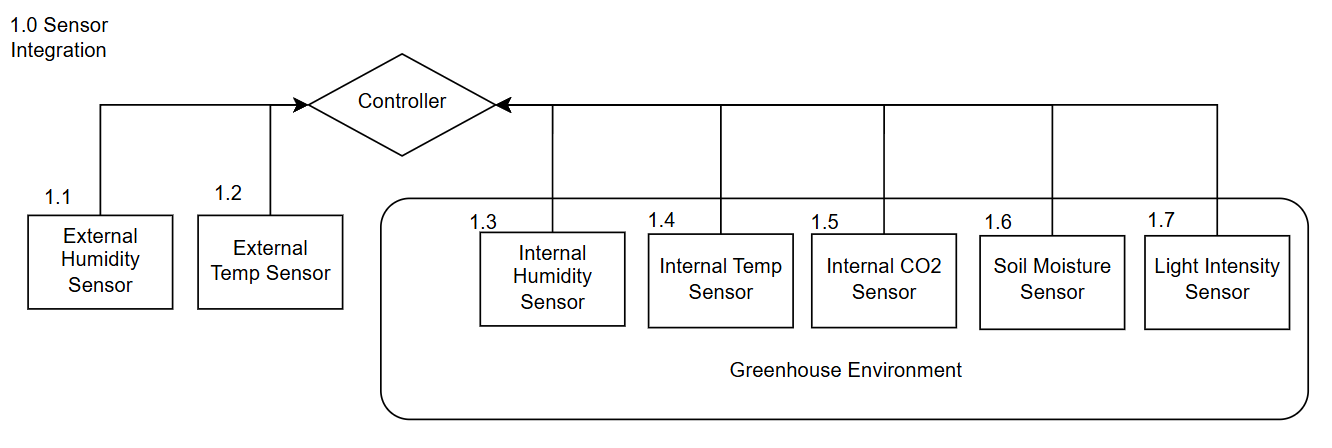
\includegraphics[width=0.8\textwidth]{figs/phys1.png}
    \caption{Sensor Physical Decomposition}
    \label{fig:sensor_decomposition}
\end{figure}

\begin{figure}[H]
    \centering
    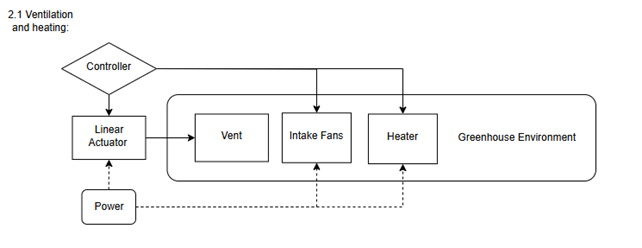
\includegraphics[width=0.8\textwidth]{figs/phys2.png}
    \caption{Ventilation Physical Decomposition}
    \label{fig:ventilation_decomposition}
\end{figure}

\begin{figure}[H]
    \centering
    \includegraphics[width=0.8\textwidth]{figs/phys3.png}
    \caption{Irrigation Physical Decomposition}
    \label{fig:irrigation_decomposition}
\end{figure}

\begin{figure}[H]
    \centering
    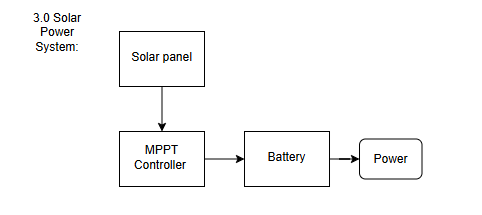
\includegraphics[width=0.8\textwidth]{figs/phys4.png}
    \caption{Solar Physical Decomposition}
    \label{fig:solar_decomposition}
\end{figure}








\chapter{Detailed Design}\label{chap:design}

This section presents the detailed greenhouse design using a structured approach: for each design element, requirements are defined first, followed by technical specifications and implementation details. A key design priority is the roof vent to maximize passive ventilation, which guided the geometry and mechanism choices that follow. Following design reviews, a revised structural design was developed to enable improved operation and manufacturability. The general shape was optimized to accommodate laser cutting processes, with the use of the universities CO2 laser cutter with a maximum available bed size of \SI{1260}{mm} $\times$ \SI{860}{mm}. The roof geometry was modified to an uneven-span lean-to configuration. While this maintains a steep roof inclination for efficient solar gain, it also allows for better thermal control and ensures that the roof vent can be actuated even when the greenhouse is positioned adjacent to a wall.

Allowing users to place the greenhouse against a thermally massive surface (e.g., a concrete or brick wall) enhances passive heat retention and improves overall energy performance. Additionally, the revised structure introduced more right angles, simplifying manufacturing and increasing the usable internal volume of the greenhouse.

\begin{figure}[h]
	\centering
	\begin{subfigure}[b]{0.43\textwidth}
		\centering
		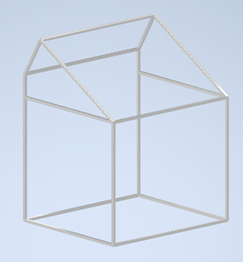
\includegraphics[width=\textwidth]{figs/frame.png}
		\caption{Frame Structure}
		\label{fig:image1}
	\end{subfigure}
	\hspace{0.6em} % was \hfill — make this small; 0pt to touch, negative to overlap
	\begin{subfigure}[b]{0.41\textwidth}
		\centering
		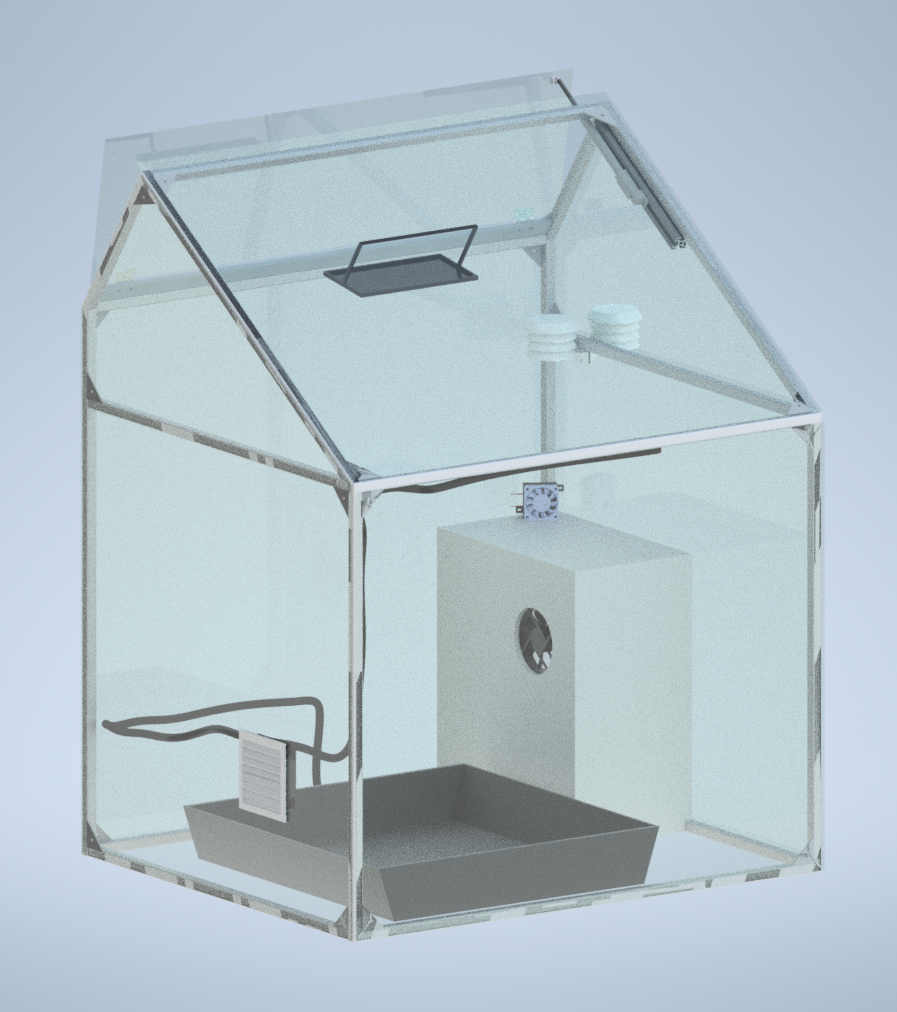
\includegraphics[width=\textwidth]{figs/front.png}
		\caption{Final Concept}
		\label{fig:image2}
	\end{subfigure}
	\caption{Detailed Design}
	\label{fig:side_by_side}
\end{figure}

\begin{figure}[H]
	\centering
	\fbox{\includegraphics[width=0.86\textwidth]{figs/anotated.png}}
	\caption{Final Concept Definition}
	\label{fig:Final_concept}
\end{figure}

The control center protecting all of the electrical components is shifted to the side of the greenhouse and a door is laser cut from the right side Perspex panel allowing easy access for maintenance. This side access preserves the ability to have the greenhouse be leveraged against an existing wall maximizing space efficiency. Hinges on the front Perspex panel enable it to open for convenient access required for planting and harvesting.


\section{Structure}
\subsection{Frame}
The frame must provide a durable structural foundation that supports the greenhouse covering material, withstands environmental loads such as wind and rain, and does so in a cost-effective manner. Aluminum square tubing is selected for its excellent strength-to-weight ratio. Compared to a stainless steel frame, aluminum offers a much lighter structure, making the greenhouse easier to transport or reposition if necessary. Additionally, aluminum is naturally corrosion-resistant, eliminating the need for protective coatings to prevent rust. Standard aluminium extrusions are also widely available and relatively easy to cut and assemble, making it a practical and cost-effective choice for the frame. A structural analysis seen in the calculations in Appendix \ref{chap:calcs} confirmed that the frame can withstand its own weight, the weight of Perspex panels, and wind loads simultaneously. The calculated safety factor for the aluminium frame, based on maximum wind loads of up to 40 km/h acting perpendicularly to the side panels, was determined to be approximately 40.1 . The maximum deflection simulated at the apex of the greenhouse amounted to only 0.5\,mm, demonstrating excellent structural stiffness and integrity. Detailed engineering drawing of the frame assmbly can be seen in Appendix \ref{fig:engineering-drawing}

\subsection{Covering material}
Perspex was chosen over glass for its combination of machinability, thermal performance, transparency, and non-brittle nature, addressing both construction and long-term durability needs.

\section{Control Center Design}
\subsection{Electrical Component Housing}
A dedicated area is required for the safe and neat storage of all electrical components such as the battery, charge controller, buck convertor, microcontroller, relays and valve. The control center can be made from wood as it is simple to construct and mount parts to, as well as being electrically nonconductive and thermally insulating. Specifically, marine plywood is used as it resists water damage and is made from high-quality hardwood veneers, making it stronger and more resistant to warping compared to standard plywood. Coating it with white exterior-grade paint will further improve water resistance and reflect sunlight, keeping internal components cooler while reflecting more light for the plants. Silicone sealant is applied in and around the control centre to ensure waterproofing and isolate it from the greenhouse environment, protecting components from misting and rain.

\begin{figure}[H]
	\centering
	\fbox{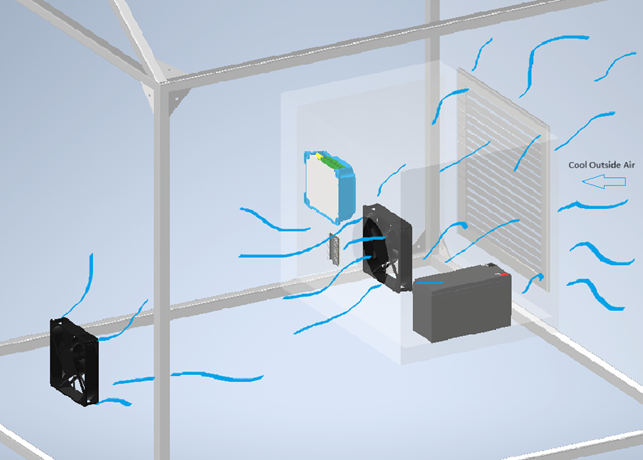
\includegraphics[width=0.65\textwidth]{figs/airflow1.png}}
	\caption{Air Intake}
	\label{fig:air_circulation}
\end{figure}

\subsection{Control Center Ventilation }
A cutout from the Perspex allows for placement of a louvre vent as seen in figure \ref{fig:air_circulation}. These vents will allow for passive ventilation to keep the control center cool while the shape of the louvre vents will prevent water from entering. This vent is placed on the side of the greenhouse to allow for the placement of the greenhouse against a wall. 

For this reason, the control center was moved to the right side of the greenhouse, freeing up more space for plants. Dedicated ventilation prevents overheating, a strategically positioned HAF fan mounted on the enclosure's side creates an airflow path drawing outside air through the large louvred vent, across the electronics, and exhausting it into the greenhouse. This dual-purpose setup cools the control and electrical components while supplying fresh air to the growing environment.

\subsection{Access Panel}
A cutout from the side panel around the control center allows for the placement of a door providing easy access to the electrical components. This door will also incorporate the louvred vent, enabling proper ventilation for the electrical components and acting as the intake for the HAF fan attached to the side of the control center.

\section{Intake and HAF fans}
Intake fans bring in fresh oxygen rich air when needed. To regulate the greenhouse temperature, cool air is drawn in from the base while a top vent opens to allow warm air to escape, promoting natural convection and effective cooling. Industrial greenhouses also rely on HAF fans to promote healthy air movement and prevent stagnation. However, on a smaller scale, dedicated HAF fans are not necessary. For the sake of simple design and using smart controller logic these two actions of air intake and HAF can be combined to be completed by the same two components. In this case two 12V fans on either side of the greenhouse are placed towards the bottom section of the greenhouse. These two fans will allow for air intake when necessary as well as intermediate HAF control at set intervals. The fans are placed slightly offset from each other to promote circular airflow and improve coverage.

\begin{figure}[H]
	\centering
	\fbox{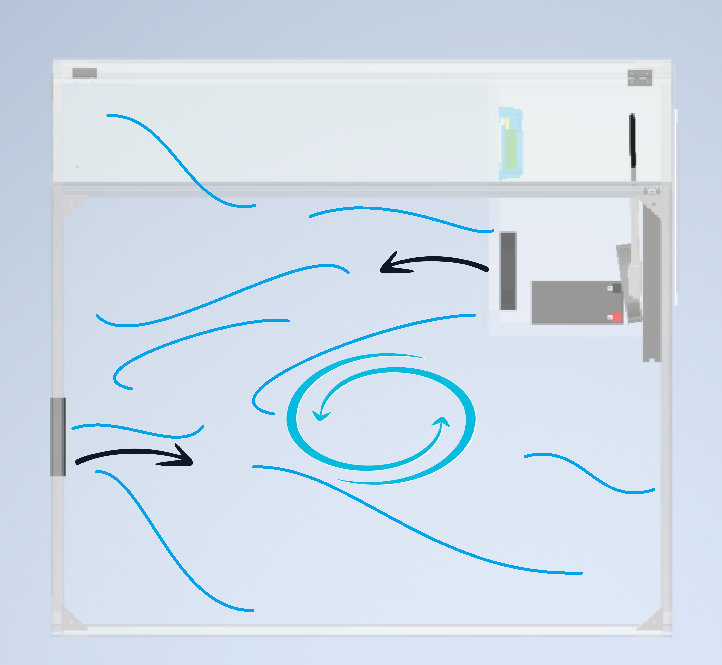
\includegraphics[width=0.5\textwidth]{figs/whirlpool.png}}
	\caption{Air circulation}
	\label{fig:air_circulation}
\end{figure}

Exhaust fans were excluded from the design as the roof vent, having a large surface area, will allow for the escape of a large quantity of air when the air intake and ventilation is active. This exhaust flow is assisted by the buoyancy effect as stipulated in the calculations in Appendix \ref{chap:calcs}

\subsection{HAF Requirements}

A common guideline is to size the HAF fans to be able to move 2 CFM for each square foot of greenhouse floor area \citep{Watson2019}. By these standards for the floor area of 0.85\,m\textsuperscript{2} an HAF capacity of at least 18.3\,CFM would be required to ensure healthy air circulation. Two 120\,mm PC fans with an average of 70\,CFM each will be more than sufficient and will be activated during dedicated HAF periods.

\begin{align}
	\small
	A_{\text{floor}} &:= b \cdot l = 0.85 \,\si{m^2} \\[1em]
	A_{\text{floor,ft}} &:= A_{\text{floor}} \cdot 10.764 \,\frac{\si{ft^2}}{\si{m^2}}
	= 9.1494 \,\si{ft^2} \\[1em]
	CFM_{\text{HAF}} &:= A_{\text{floor,ft}} \cdot 2 \,\frac{\si{ft}}{\si{min}}
	= 18.2988 \,\frac{\si{ft^3}}{\si{min}}
\end{align}

Due to the use of misting systems within the greenhouse care needs to be taken to protect the fans and other components from moisture buildup, for this reason 3D printed covers and louvered vents are designed to protect from droplet buildup on components. Smart placement of misting nozzles and intermediate misting control will also prevent excessive moisture exposure to electrical components.

\section{Ventilation}

\subsection{Natural Ventilation}

An effective ventilation system at the top of the greenhouse will allow for passive cooling using the buoyancy effect of the warm air within the greenhouse. The larger the area of the vent the more effective the air transfer and thus cooling capabilities. A Perspex panel on the roof measuring 1000mm by 270mm is to be actuated to the open position to allow for this exchange. A linear actuator is selected as it is less complicated than installing a motor and shaft and more cost effective. The actuator selected should have a large stroke of at least 100mm to increase the opening area and will need to be rated to lift the weight of the Perspex panel. Calculations seen in Apendix \ref{chap:calcs} were completed to ensure that the specification can be met and an example can be seen in the free body diagram below. 

\begin{figure}[H]
	\centering
	\fbox{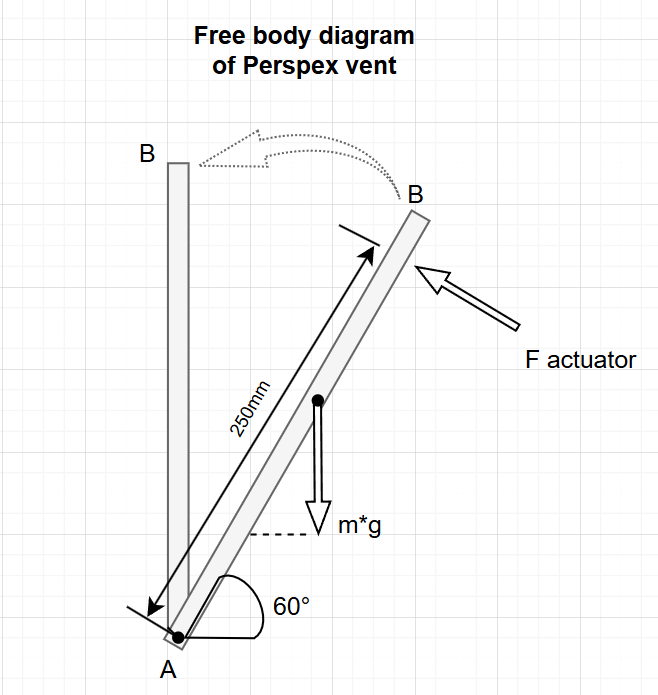
\includegraphics[width=0.3\textwidth]{figs/fbd.png}}
	\caption{Free body diagram of Vent Mechanism}
	\label{fig:vent_fbd}
\end{figure}

When opened, the vent exposes the greenhouse interior to potential precipitation, which could result in overwatering or water exposure to electrical components. To mitigate this, a rain sensor is mounted on the exterior of the greenhouse and connected to the microcontroller. When moisture is detected, the sensor signals the system to close the vent, thereby protecting both the plants and internal electrical components during periods of rain.

\subsection{Forced Ventilation}
 
Typical greenhouse design guidelines recommend approximately one complete air exchange per minute \citep{Watson2019}. With a greenhouse volume of 0.77~m$^3$, this requires two fans with a combined flow rate of at least 0.77~m$^3$/min. Calculations in Appendix \ref{chap:calcs} indicate that the volumetric flow rate of the intake fans must be at least 27~CFM. Accordingly, two PC fans, each averaging 70~CFM, are selected, more than sufficient to exchange the entire greenhouse volumes air within one minute.

\section{Misting System}

Effective greenhouse environmental control requires regulating soil moisture while maintaining relative humidity (RH) within crop-specific setpoints. To avoid the complexity of parallel systems, this design adopts a single misting system coordinated by scheduling and control procedures to handle both irrigation and humidity management. When irrigation or a misting cycle elevates RH, the mechanical ventilation is automatically engaged to exhaust excess moisture and restore RH to the target range. The developed control algorithms for this optimization can be seen in appendix \ref{flow}. A further advantage of the misting system is evaporative cooling, which operates in combination with the greenhouse’s passive (roof vent) and active ventilation to limit temperature spikes above desired thresholds.

Misting Nozzles are placed effectively to ensure moisture reaches the roots directly. Up to 4 nozzles are placed slightly above the soil and deliver water straight to the soil medium. Misting nozzles offer adjustable spray patterns, ranging from a targeted drip to an ultra-fine mist. Two additional nozzles will be installed at a higher elevation within the greenhouse to provide broader coverage while still targeting specific zones. Careful positioning will ensure mist is directed away from sensitive electrical components. 

\section{Active Heating System}
To achieve effective active heating, a fan heater is selected. Based on the heat loss calculations on the surface area, the greenhouse experiences a convective heat loss of approximately 119\,W when there is a 5\,°C temperature difference between the internal and external environments. 

Given that many plants require a minimum desirable temperature of around 15\,°C for optimal growth, the heating system must be capable of compensating for this heat loss. Therefore, a fan heater with a power rating of at least 120\,W is required.

A 12,V, 120,W fan heater is provided by the university to meet this requirement, powered directly by the 12,V battery supply. The heater is controlled via a relay module, which is switched by signals from the microcontroller. This setup allows the heater to automatically activate when the internal temperature falls below a user-defined threshold. A hysteresis band is implemented in the code, this prevents fast unnecessary switching, allowing for accurate feedback and extending the lifespan of the heater and relays.


\section{Environmental Monitoring}
\label{sec:environmental_monitoring}
The greenhouse uses a network of environmental sensors connected to a central microcontroller to continuously monitor key parameters such as temperature, humidity, soil moisture, light intensity, and CO\textsubscript{2} concentration. These measurements provide real-time feedback on the internal climate conditions, which are essential for optimizing plant health and growth. 

The data collected is processed by the microcontroller and used both for local decision-making (e.g., activating ventilation or irrigation systems) and for remote monitoring via IoT platforms. Through cloud-based interfaces, users can access historical data and current conditions, and adjust system settings as needed. The following sections detail the selection and implementation of the microcontroller, the individual sensors, and the data acquisition platforms used in the system.

\subsection{Controller}
\label{subsec:controller}
The ESP32 microcontroller, developed by Espressif, is selected for its abundant I/O options, making it ideal for managing multiple sensors and actuators through its numerous GPIO pins. Its built-in Wi-Fi and Bluetooth connectivity enables seamless communication with user interfaces, allowing for real-time monitoring of the greenhouse environment.

The ESP32 supports a variety of communication protocols such as I\textsuperscript{2}C, UART, and SPI, allowing seamless integration with environmental sensors and control modules. Its dual-core processing power ensures efficient real-time data handling and decision-making. Its integration with Arduino's IDE software allows for easy programming capabilities. Additionally, the ESP32's low power consumption and wide community support make it a reliable and cost-effective choice for an embedded greenhouse controller.

\subsection{Sensors}
\label{subsec:sensors}
Multiple sensors enable accurate monitoring of both the internal greenhouse environment and the external ambient conditions. This data informs the control of greenhouse parameters and provides a baseline for comparison between internal and external climates. 

The external temperature and humidity sensor will be exposed to direct sunlight and rainfall, while the internal sensors will experience both sunlight and periodic misting. To ensure longevity and reliable performance, protective housings are required. Custom 3D-printed Stevenson screens can shield sensors from water and heat while allowing airflow through their slatted design for accurate readings. White filament is recommended to reflect sunlight and minimize heat absorption. In accordance with standards, the Stevenson screen should be mounted around 1.2m above ground level~\cite{manclim}.

\begin{figure}[htbp]
	\centering
	\fbox{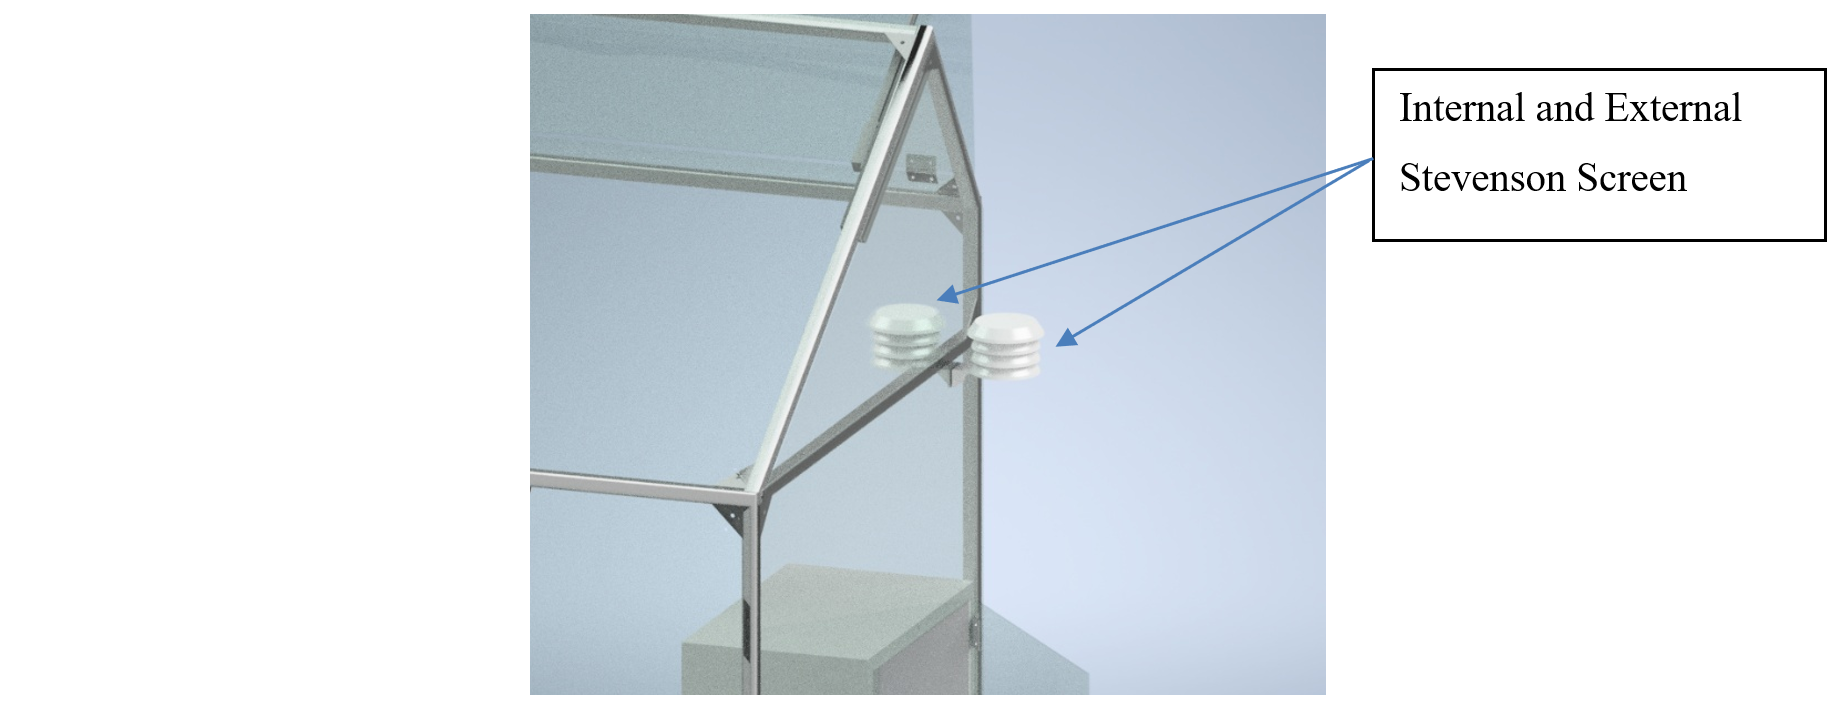
\includegraphics[width=0.9\textwidth]{figs/steven.png}}
	\caption{Stevenson Screens for sensor protection}
	\label{fig:stevenson_screens}
\end{figure}

The following sections break down each sensor's selection and operation.

\subsubsection{ Temperature and Humidity Sensor}

The DHT22 sensor was selected for its balance of accuracy, low cost, and ease of integration. Since it measures both temperature and relative humidity, it reduces the need for separate sensors, streamlining wiring and system design. It communicates with the ESP32 using a single-wire digital interface, making implementation straightforward.

\begin{table}[H]
	\centering
	\caption{DHT22 Temperature and Humidity Sensor Specifications}
	\label{tab:dht22_specs}
	\begin{tabular}{ll}
		\toprule
		\textbf{Parameter} & \textbf{Specification} \\
		\midrule
		Temperature Range & -40 to 80\,$^\circ$C \\
		Temperature Accuracy & $\pm$0.5\,$^\circ$C \\
		Humidity Range & 0--100\,\% RH \\
		Humidity Accuracy & $\pm$2--5\,\% RH \\
		Operating Voltage & 3.3--5.5\,V \\
		Output Signal & Digital (single-wire protocol) \\
		\bottomrule
	\end{tabular}
\end{table}


\subsubsection{ Light Sensor}
The BH1750 light sensor is chosen for its good balance of accuracy, cost-effectiveness, and ease of integration. It provides precise ambient light measurements in lux, making it suitable for monitoring plant lighting conditions with a simple conversion to PPFD values. It’s I²C communication protocol allows seamless and reliable connection with the ESP32, using only two GPIO pins. The sensor also requires minimal configuration and is supported by well-documented libraries, enabling quick setup and consistent performance in greenhouse environments.

\begin{table}[h]
	\centering
	\caption{BH1750 Light Sensor Specifications}
	\label{tab:bh1750_specs}
	\begin{tabular}{ll}
		\toprule
		\textbf{Parameter} & \textbf{Specification} \\
		\midrule
		Operating Voltage & 3.3-5V \\
		Interface & I\textsuperscript{2}C (7-bit address: 0x23 or 0x5C) \\
		Measurement Range & 1--65,535\,lx \\
		Resolution & 1\,lx (High-Resolution Mode) \\
		Accuracy & $\pm$20\% at 25$^\circ$C \\
		Current Consumption & $\approx$0.12\,mA (active), 0.01 \\
		\bottomrule
	\end{tabular}
\end{table}


\subsubsection{ Carbon Dioxide Sensor}
The MH-Z19 CO\textsubscript{2} sensor is chosen due to its balance of affordability, accuracy, and ease of integration with microcontrollers like the ESP32. It uses Non-Dispersive Infrared (NDIR) technology to detect CO\textsubscript{2} concentrations, which provides reliable and stable readings with minimal calibration necessary.

The sensor communicates through UART or PWM, offering flexibility in how data is read by the system. Its compact design and low power consumption (typically 33\,mA at 5\,V) make it ideal for continuous indoor monitoring in environments such as greenhouses. The sensor has a measurement range of 0--5000\,ppm with an accuracy of ±(50\,ppm + 5\% of reading) in the 0--2000\,ppm range.

\begin{table}[H]
	\centering
	\caption{MH-Z19 CO\textsubscript{2} Sensor Specifications}
	\label{tab:mhz19_specs}
	\begin{tabular}{ll}
		\toprule
		\textbf{Parameter} & \textbf{Specification} \\
		\midrule
		Communication & UART, PWM \\
		Operating Voltage & 3.6--5.5\,V \\
		Current Consumption & 33\,mA (typical) \\
		Measurement Range & 0--5000\,ppm \\
		Accuracy & ±(50\,ppm + 5\% of reading) \\
		Warm-up Time & 3 minutes \\
		\bottomrule
	\end{tabular}
\end{table}


\subsubsection{ Soil Moisture Sensor}
\label{subsubsec:soil_moisture}
The soil moisture sensor needs to provide real-time monitoring of substrate hydration levels, enabling the automated misting system to deliver precise irrigation when needed. A generic industrial grade capacitive soil moisture sensor and module is selected for its simplicity, cost-effectiveness, and compatibility with the ESP32 microcontroller.

\begin{table}[h]
	\centering
	\caption{SEN0114 Soil Moisture Sensor Specifications}
	\label{tab:sen0114_specs}
	\begin{tabular}{ll}
		\toprule
		\textbf{Parameter} & \textbf{Specification} \\
		\midrule
		Output Signal & Analog voltage \\
		Operating Voltage & 3.3--5\,V \\
		Interface & 1-wire (requires ADC) \\
		Probe Material & Corrosion-resistant alloy \\
		Measurement Depth & Up to 37\,mm \\
		\bottomrule
	\end{tabular}
\end{table}

The sensor operates by measuring the conductivity between two exposed probes inserted into the soil, where higher conductivity indicates greater moisture content. It provides an analog voltage output (0--3.3\,V) corresponding to the soil's moisture level, allowing for real-time monitoring of water content in the growing medium. 

The sensors ease of integration and low power requirements (drawing less than 20\,mA) make it well-suited for irrigation automation. The sensor only requires one wire for communication and connects to an analog-to-digital converter (ADC) pin on the ESP32. Initial calibration is required to establish the relationship between voltage output and actual soil moisture content. This can be achieved as follows. 

\subsubsection*{Calibration Procedure}

\begin{enumerate}
	\item \textbf{Hardware Setup:} Connect the soil moisture sensor's output to an ADC compatible pin (e.g., GPIO 11) set to 12-bit resolution on the ESP32. Ensure the sensor is powered correctly.
	
	\item \textbf{Wet Point Calibration:} Place the sensor probes in fully saturated soil (considered 100\% moisture). Record the stable ADC reading, \( R_{\text{wet}} \).
	
	\item \textbf{Dry Point Calibration:} Place the sensor probes in completely dry soil (considered 0\% moisture). Record the stable ADC reading, \( R_{\text{dry}} \).
	
	\item \textbf{Software Implementation:} In the microcontroller code, map subsequent ADC readings (\( R \)) to a percentage value using the following linear interpolation formula:
	
	\begin{equation}
		\text{Moisture Percentage} = \left( \frac{R - R_{\text{dry}}}{R_{\text{wet}} - R_{\text{dry}}} \right) \times 100\%
	\end{equation}
\end{enumerate}

\subsubsection{ Rain Sensor}

A rain sensor is mounted on the exterior of the greenhouse to detect rainfall and trigger protective actions. When rainfall is detected, the system is programmed to automatically close the ventilation openings, thereby safeguarding electrical components and preventing overwatering of the plants. 

The selected model is an HKD general-purpose rain sensor, which features a large sensing surface to improve droplet detection. The sensor operates by using exposed conductive tracks on the board: when water bridges the tracks, the resistance changes significantly, from approximately \SI{2}{\mega\ohm} when dry to around \SI{100}{\kilo\ohm} when wet. This variation is processed by the module, which outputs a digital signal (logic HIGH or LOW) to indicate the presence of rain. 



\subsection{Data Acquisition and Monitoring}
\label{subsec:data_acquisition}


The ESP32 can collect sensor data and store it locally in .xls format on an SD card. However, to provide a more accessible and user-friendly interface, data will instead be uploaded to a cloud-based platform such as ThingSpeak. ThingSpeak supports monitoring and control of up to 8 fields with a minimum update interval of 15 seconds. The free tier offers up to 3 million messages per year, which equates to approximately 8,000 messages per day. Blynk is another free IoT platform that allows for easy creation of mobile apps to control and monitor hardware remotely. It is fully compatible with the Arduino platform, making it a convenient choice for IoT projects. A Blynk dashboard is thus setup alongside a ThingSpeak dashboard to allow for wireless monitoring and control of the greenhouse environment.

\begin{figure}[H]
	\centering
	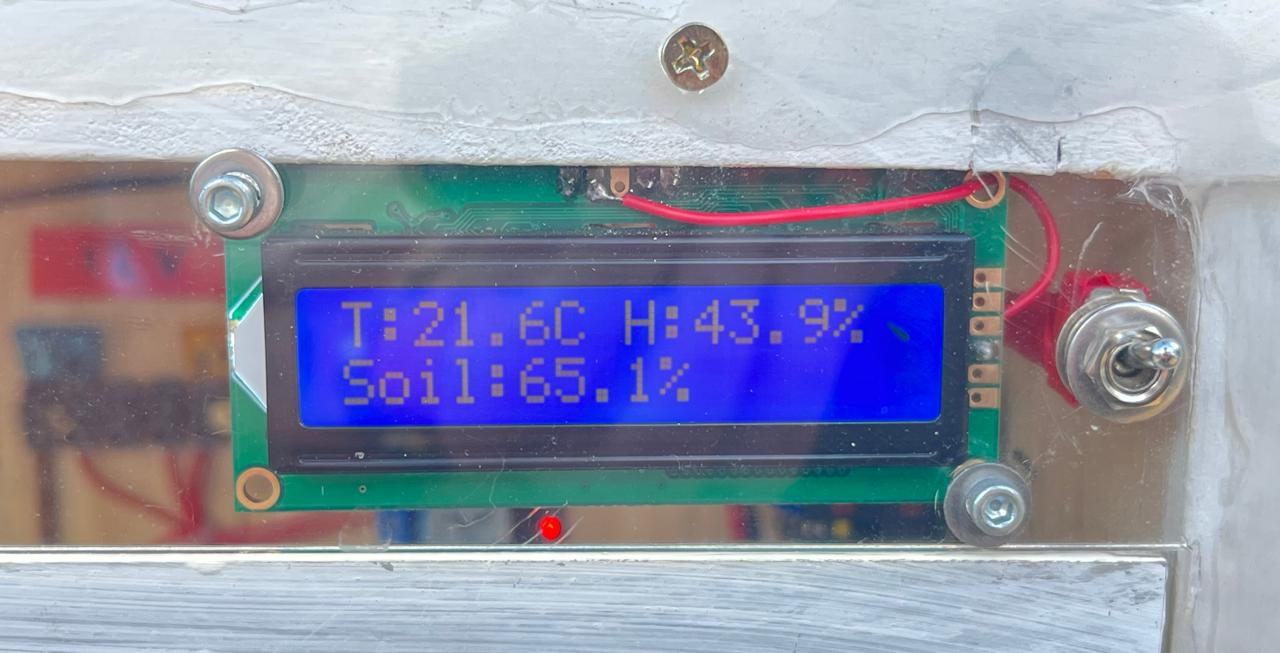
\includegraphics[width=0.5\textwidth]{figs/LCD.jpg}
	\caption{LCD screen for local monitoring}
	\label{fig:lcd_screen}
\end{figure}

\subsubsection*{Local Monitoring}
\label{subsubsec:local_monitoring}
Local monitoring is useful when a user is on-site near the greenhouse and wants to easily view the current internal conditions. Additionally, in the event of a Wi-Fi outage, the greenhouse can still communicate essential data locally. For this reason, a small LCD screen is used to display key environmental parameters, including temperature, humidity, light levels, soil moisture, and CO\textsubscript{2} concentration. The LCM1602A display is selected for its built-in I\textsuperscript{2}C communication interface. 
This allows it to share the same two pins already used by the BH1750 sensor, since I\textsuperscript{2}C supports multiple devices on a single bus through unique addresses. 
The LCM1602A operates at address \texttt{0x3E}, enabling efficient integration while reducing GPIO pin usage compared to the standard 8-bit parallel interface.
The screen cycles through these readings to present the information clearly and efficiently. It is mounted above the control room door and is visible through the Perspex panel, allowing for quick visual access without needing to enter the enclosure. The active screen alongside the all purpose on/off switch can be seen in the figure above.


\section{Power Supply}
\label{sec:power_supply}
The power supply provides energy to the system as a whole and is crucial for the general operation and reliable functioning of the device. Power is supplied by a 12\,V battery through the integration of a barrel jack. However, several components require 5\,V or 3.3\,V for operation. Therefore, voltage conversion is necessary to supply the correct operating voltages. Instead of a traditional linear voltage regulator, a buck converter is chosen for its higher efficiency, especially when stepping down from 12\,V. Two fuses are incorporated to safeguard the components against potential failures or voltage spikes. 
Following the guideline of using 1.5 times the maximum expected current, a 15\,A fuse is installed to protect the 12\,V line, supplying high-power components such as the solenoid valve and heater. 
Additionally, a smaller 5\,A fuse is placed on the supply line to the buck converter, ensuring protection for the lower-power electronics operating at 5\,V and 3.3\,V.

\subsection{Step-down Buck Converter}

A buck converter is a type of DC-DC converter that efficiently reduces a higher input voltage to a lower output voltage using high-frequency switching elements (typically a transistor and a diode) along with energy storage components like inductors and capacitors. This method significantly reduces power loss compared to linear regulators, which dissipate excess voltage as heat.

For this application, an MP4560 buck converter module is used. It is a high-efficiency, step-down switching regulator capable of handling input voltages up to 36V and outputting up to 3A. It is configured to provide a steady 5V output, which is distributed via a 5V rail for convenient access by various components. The MP4560 features an integrated high-side switch, built-in thermal protection, and short-circuit protection, making it well-suited for embedded applications.

An LED is included in the 5V power circuit to indicate active power supply, giving the user a visual cue that the system is powered. In accordance with the MP4560’s datasheet recommendations, decoupling capacitors are placed on both the input and output to stabilize voltage and suppress noise. These capacitors serve to filter out voltage ripples and transient fluctuations by storing charge and releasing it when needed, ensuring clean and stable voltage to connected components.

\subsection{Battery Capacity}

A battery capacity of at least 89Ah is required to power the average energy usage of the system and its components as shown in the calculations in Appendix \ref{chap:calcs}. The calculations provide for an allowable minimum depth of discharge (DoD) of 20\% for recommended safe sealed gel battery usage. A battery with a capacity of 100Ah is provided by the university to meet the requirements.

\subsection{Solar System}

A solar system rated to provide at least 240W would be able to charge the battery fully in one day assuming a moderate system efficiency of 80\% as shown in the calculations. Thus a single solar panel of at least 240W or two 120W panels can be sourced. 

\subsection{Provided Equipment}\label{sec:provided}

The M\&M department of engineering has provided a 12V, 100Ah battery which should be sufficient based on the previous DoD calculations. Additionally two solar panels rated at 105W are provided along with a MPPT Skyking Solar Charge Controller. This charge controller will charge the battery from the 2 solar panels which will power all the components. 

\section{Relays}
The ESP32 operates with 3.3V digital logic, which is suitable for interfacing with most sensors. However, it cannot directly control components that require higher voltages or draw significant current. To address this, relay modules are used to enable the ESP32 to switch high-power devices using low-voltage control signals. Two 4-channel relay modules have been selected for this project, capable of switching loads up to 250V and 10A, and compatible with 3.3V logic levels. This module will allow the ESP32 to control 12V devices such as fans, the linear actuator, and the heater efficiently and safely. 

\section{Linear actuator and H-Bridge}

To actuate the roof vent, a linear actuator is required. The Actuonix L16 S linear actuator is selected for this purpose due to its 12V operating voltage, its availability, and ability to deliver up to 50N of force, verified through the calculations to be more than sufficient to lift the perspex panel. The actuator includes built-in limit switches that stop motion at full extension or retraction. To control both extension and retraction, the polarity of the 12V power supply must be reversed. For this reason, an H-bridge circuit is necessary. Instead of using a dedicated H-bridge driver, the design implements two switching relays wired in an H-bridge configuration.  By toggling the relays, the polarity of the 12V supply to the actuator can be reversed, enabling both extension and retraction. Careful coding is essential to ensure that both relays are never activated simultaneously, as this could create a short circuit across the supply. Proper logic sequencing in the microcontroller program guarantees safe operation while maintaining reliable control of the actuator. 3D-printed components can be used to mount the linear actuator to the Perspex panels, providing two degrees of freedom to accommodate slight pivoting during extension and retraction.

\section{Solenoid valve}

A solenoid valve operates using an electromagnetic coil that converts electrical energy into mechanical motion. \cite{solenoid} When the coil is energized, it generates a magnetic field that moves a plunger or valve mechanism, opening or closing the fluid passage. This enables precise electronic control of water flow in irrigation systems. 

The solenoid valve is used to automate watering within the greenhouse. It is powered from the 12V supply and controlled via one of the relay channels, allowing the ESP32 microcontroller to activate the valve as needed without directly handling high current loads. The integration of a solenoid valve ensures reliable, repeatable irrigation control, enabling system automation and reducing manual intervention. 

\chapter{System Integration}

This section of the report outlines the plan for integrating both the physical hardware components and the software architecture of the greenhouse system. It begins with the wiring layout of all electronic components, followed by a description of the software framework and control logic that will govern the system operation. This section on system integration demonstrates how the various subsystems, sensors, actuators, and controllers, work together to achieve the overall functionality of the greenhouse. It also provides a clear roadmap for implementation, troubleshooting, and future scalability.

\section{Wiring}

The battery provides a 12V power rail to any components that require it. This 12V supply is connected to the Common (COM) terminals of the relay module. When activated by the microcontroller, each relay allows current to flow from the COM terminal to the Normally Open (NO) terminal, supplying 12V to the connected device. On the input side of the relay module, the VDD pin must be connected to a 5V power source, and the GND pin to ground. The four input pins labeled IN1–IN4 are connected to general-purpose I/O (GPIO) pins on the microcontroller, specifically GPIO 38,37,47 and 48, allowing the relays to be toggled via 3.3V logic signals.

These relays control the 12V-powered components: airflow fans, heater fan, grow light, and solenoid valve. Each of these devices requires a connection to ground on their negative terminal, which is wired to the negative terminal of the battery. A common ground rail ensures all components share the same electrical ground reference. The wiring schematic can be seen in the figure below


\begin{landscape}
	\begin{figure}[p]
		\centering
		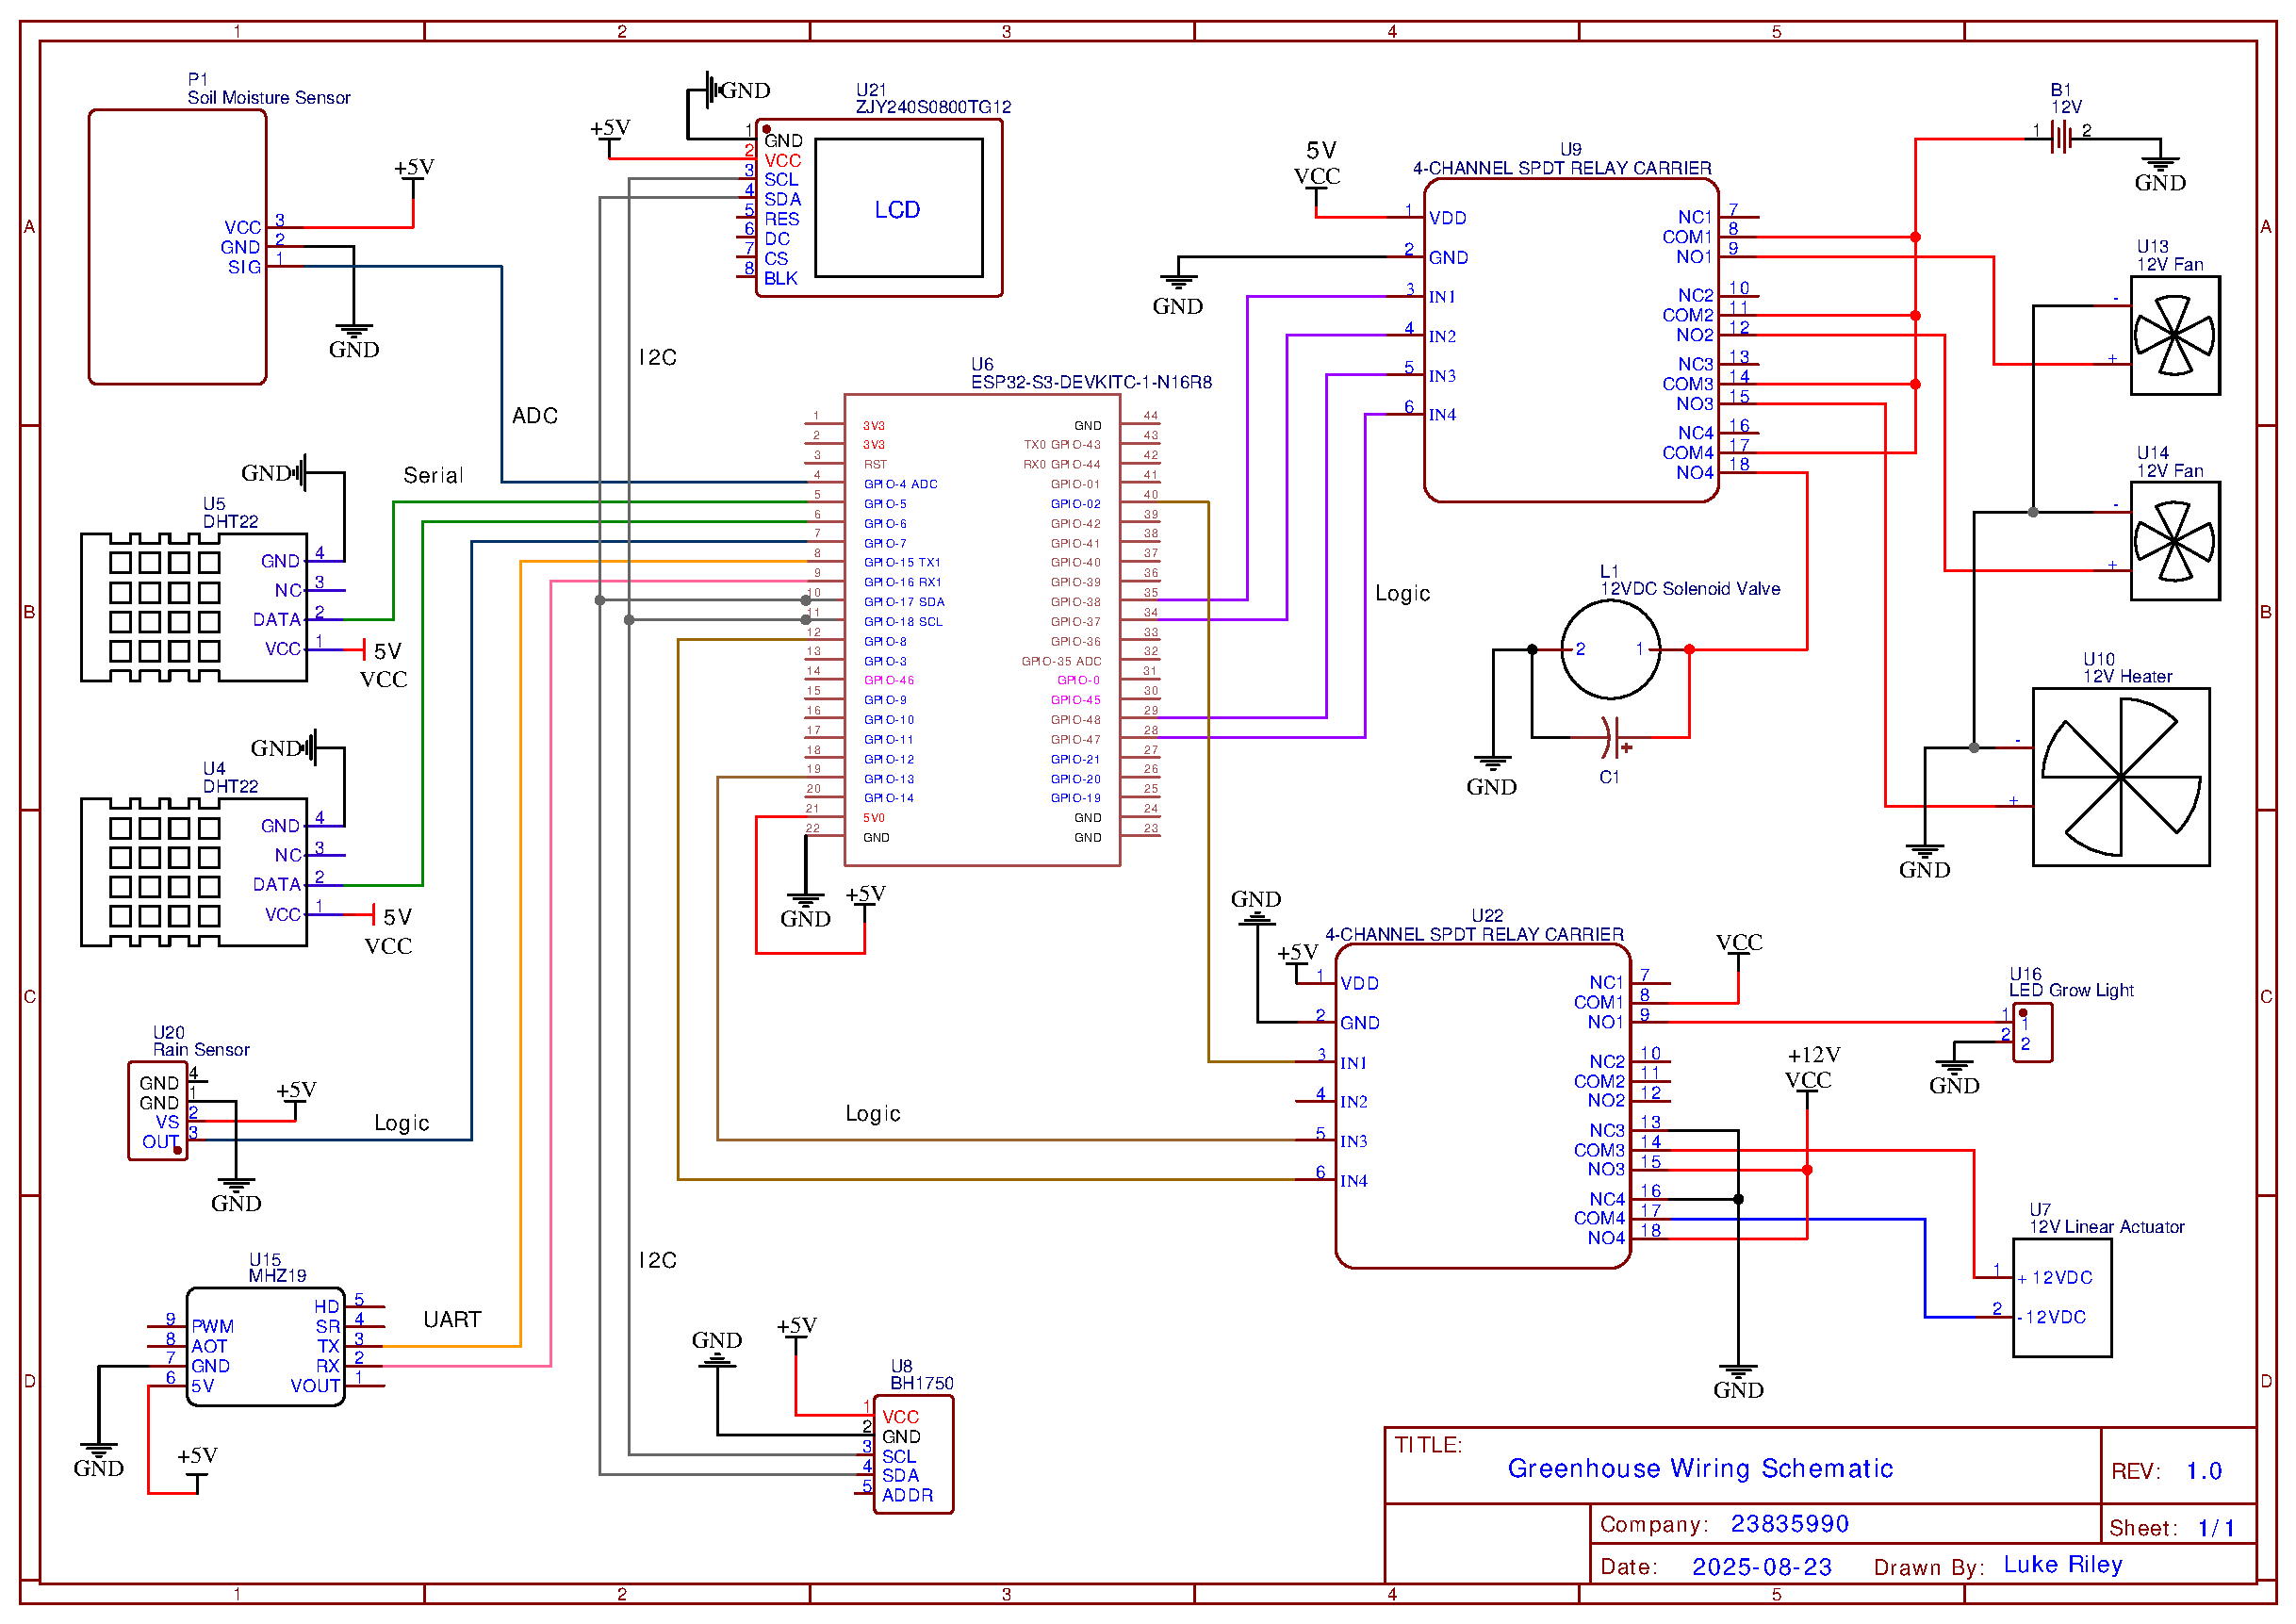
\includegraphics[width=\linewidth]{figs/wiringpd.pdf}
		\caption{Wiring schematic}
		\label{fig:lcd_screen}
	\end{figure}
\end{landscape}

For the linear actuator, bidirectional motion is achieved by reversing the polarity of the supply voltage using two channels of the relay module. GPIO 8 and GPIO 13 of the microcontroller are connected to input pins IN3 and IN4 of the relay module, respectively. The 12V supply is wired to the Normally Open (NO) terminals of both relays, while the actuator leads are connected to the Common (COM) ports. The Ground connection is tied to the Normally Closed (NC) terminals of each relay. With this configuration, switching the relays in different states alternates the polarity applied to the actuator, enabling both extension and retraction.

Other components and sensors require a 5V supply. A buck regulator is used to step down the 12V input efficiently, avoiding the high energy loss associated with voltage dividers. The regulator’s VIN is connected to the 12V rail, and its GND pins are tied to ground. The VOUT pin is connected to a 5V power rail that supplies all 5V-dependent components. Before connecting any loads, the regulator should be calibrated by measuring the output with a multimeter and adjusting the onboard potentiometer until the desired 5V output is reached.

The DHT22 sensors each require a 5V VCC connection, ground to GND, and a data line connected to GPIO 5 and 6 respectively, using digital communication. The soil moisture sensor is similarly powered with 5V to VCC, ground to GND, and its data line connected to GPIO 4. The BH1715 light sensor communicates via the I\textsuperscript{2}C protocol and is connected to 5V and ground, with SDA and SCL lines wired to GPIO 17 and 18 respectively. The rain sensor outputs a logical high coltage level of 3,3V when water is deticted, accordingly GPIO 7 is set as an input pin to read the logic level. The CO\textsubscript{2} sensor requires a 5V supply to its 5V pin, GND to ground, and TX/RX lines connected to UART-compatible GPIO pins—GPIO 15 and 16 in this case.

For local display of environmental readings, an I²C LCD module is used. The module requires 5V on its VCC pin and ground on GND. Communication with the microcontroller is achieved via the I²C protocol, with GPIO 17 connected to the SDA line and GPIO 18 to the SCL line. This configuration reduces the number of required connections compared to a parallel LCD, while still enabling reliable display of real-time sensor data. A wiring schematic is provided below.

\section{Software Framework and Control Logic}

This section outlines the software design framework for the greenhouse system. The accompanying flowcharts illustrate the sequence of tasks and decision-making processes implemented on the microcontroller. These flowcharts serve to simplify the development of complex control algorithms—particularly those involving multiple variables with competing operational requirements.

In certain situations, control actions are prioritized based on environmental conditions. For example, if the internal temperature exceeds the setpoint while soil moisture levels remain adequate, the misting system may still be activated to assist with cooling. In such cases, temperature regulation is prioritized over soil moisture conservation.

The control logic is structured into distinct modules, arranged in approximate order of priority: \textit{Principal Control}, \textit{Temperature Control}, \textit{Airflow Control}, \textit{Humidity Control}, \textit{Lighting Control}, and \textit{Air Quality Control}.

\begin{figure}[H]
\centering
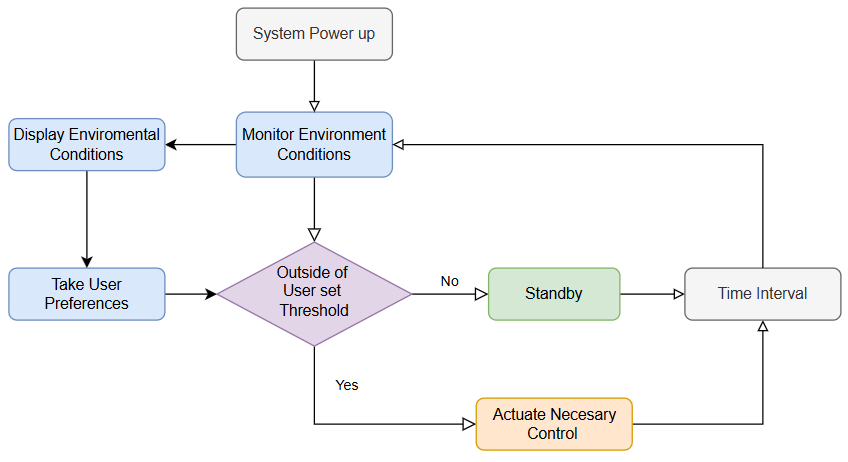
\includegraphics[width=0.85\textwidth]{figs/soft1.png} % Update path/filename as needed
\caption{Principal Control Flowchart}
\label{fig:principle_control_flowchart}
\end{figure}

Principal Control involves monitoring internal and external environmental conditions, to inform decisions about which components need to be actuated in response to undesirable conditions. These environmental readings are displayed to the user, who can then set custom threshold values based on the specific requirements of the plants being cultivated. When any measured condition falls outside the user-defined thresholds, the system responds by activating the appropriate control mechanisms. If no user preferences are provided, the system defaults to a broad, general-purpose set of control setpoints suitable for common plant types.

\begin{figure}[htbp]
    \centering
    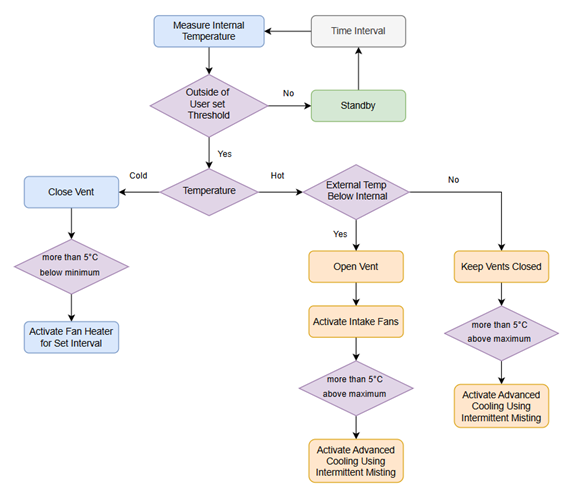
\includegraphics[width=0.8\textwidth]{figs/soft2.png}
    \caption{Temperature control}
    \label{fig:temperature_control}
\end{figure}

\begin{figure}[htbp]
    \centering
    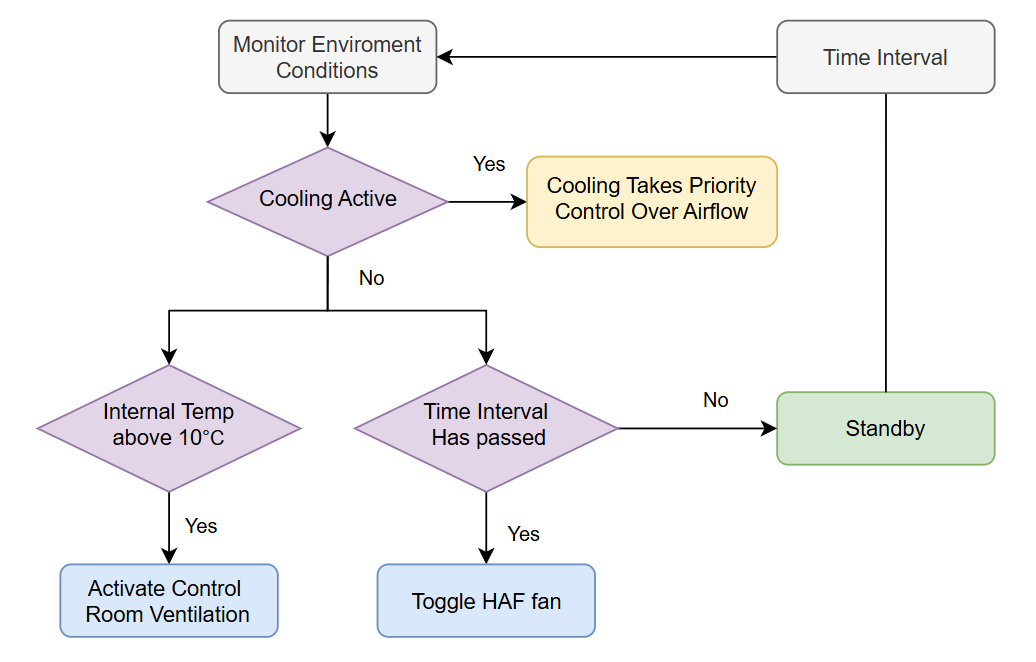
\includegraphics[width=0.7\textwidth]{figs/soft3.png}
    \caption{Airflow control}
    \label{fig:airflow_control}
\end{figure}

\begin{figure}[htbp]
    \centering
    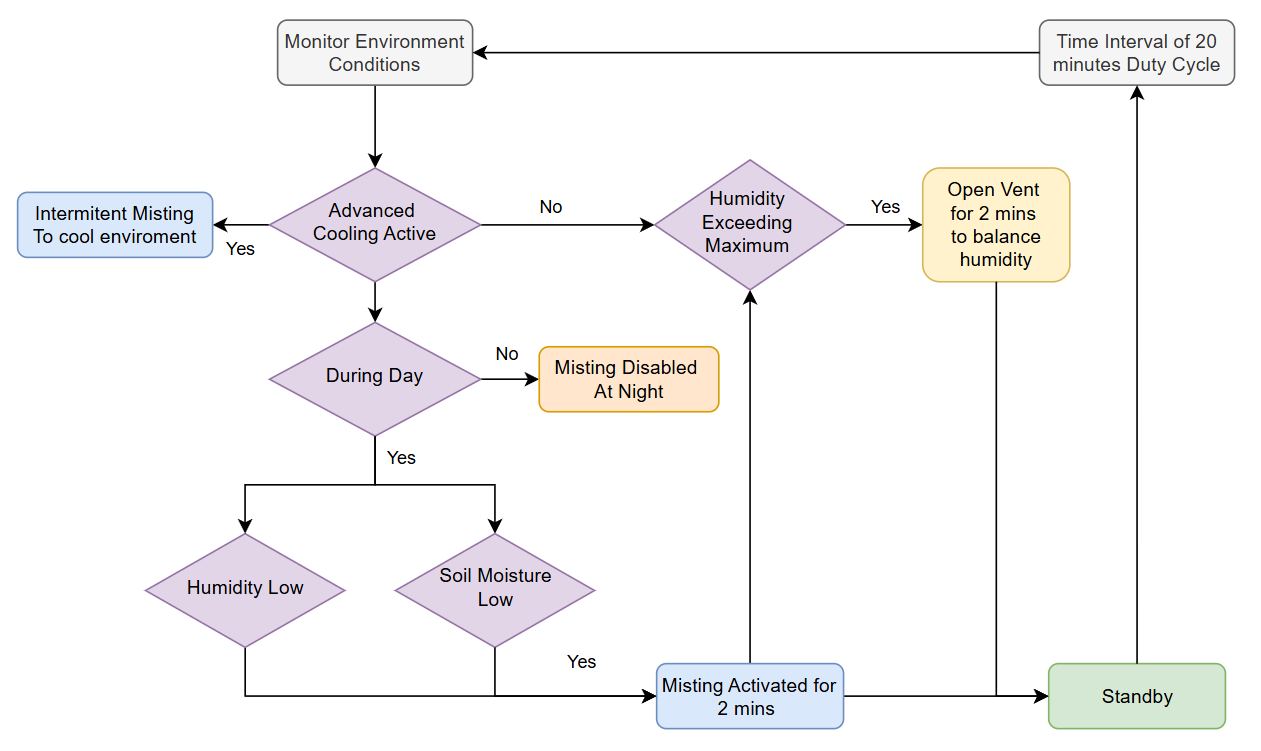
\includegraphics[width=0.8\textwidth]{figs/soft4.png}
    \caption{Irrigation control}
    \label{fig:irrigation_control}
\end{figure}

\begin{figure}[htbp]
    \centering
    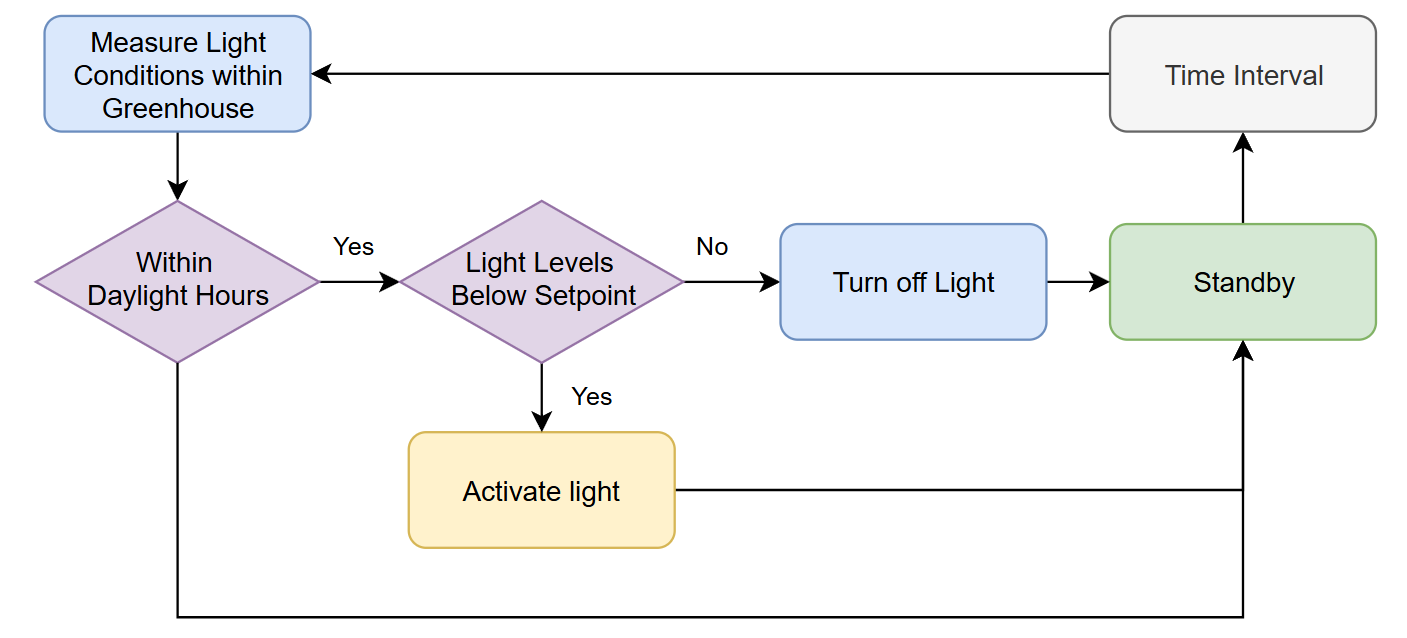
\includegraphics[width=0.7\textwidth]{figs/soft5.png}
    \caption{Light control}
    \label{fig:light_control}
\end{figure}

\begin{figure}[htbp]
    \centering
    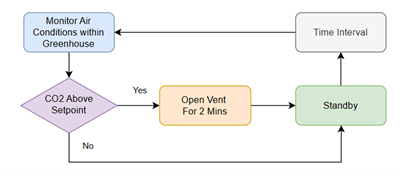
\includegraphics[width=0.6\textwidth]{figs/soft6.png}
    \caption{Air quality Control}
    \label{fig:air_quality_control}
\end{figure}

The inclusion of these flowchart diagrams streamlines the programming of the microcontroller's control logic by providing a clear framework for implementation, reducing the likelihood of debugging issues caused by conflicting decision-making processes.
\chapter{Design Evaluation}\label{chap:eval}

This section outlines the tests used to validate the greenhouse systems setup and operation. It includes performance tests to validate selection and design of sensors, actuators the system as a whole and its wireless monitoring and control capabilities. 

\section{Sensor Validation}\label{sec:sensor_validation}

All sensors were tested to verify their response and accuracy to real environmental changes under controlled conditions.  Each was connected to the ESP32 microcontroller with the appropriate pin configuration, and real-time data was logged at one-second intervals through serial communication. 
The data was imported into MATLAB for processing and visualization. 
This setup ensured consistent testing and provided clear insight into each sensor’s performance characteristics.

\subsection{Temperature and Humidity Sensor (DHT22)}

\subsubsection*{Test Objective}
The purpose of this test was to verify the accuracy and responsiveness of the DHT22 sensor to real environmental changes in temperature and humidity. 

\subsubsection*{Methodology}
The sensor was connected to the ESP32 microcontroller through serial comunication and live readings were recorded. 
A burst of warm air was directed towards the sensor to simulate a rapid change in environmental conditions. 
The corresponding temperature and relative humidity values were logged and plotted using MATLAB for analysis. 

\subsubsection*{Results}
The plotted data, shown in Figure~\ref{fig:dht22_test}, demonstrates the sensor's response to the applied stimulus. 
A clear rise in temperature was observed immediately after exposure to warm air, accompanied by a corresponding change in humidity. 

\begin{figure}[H]
	\centering
	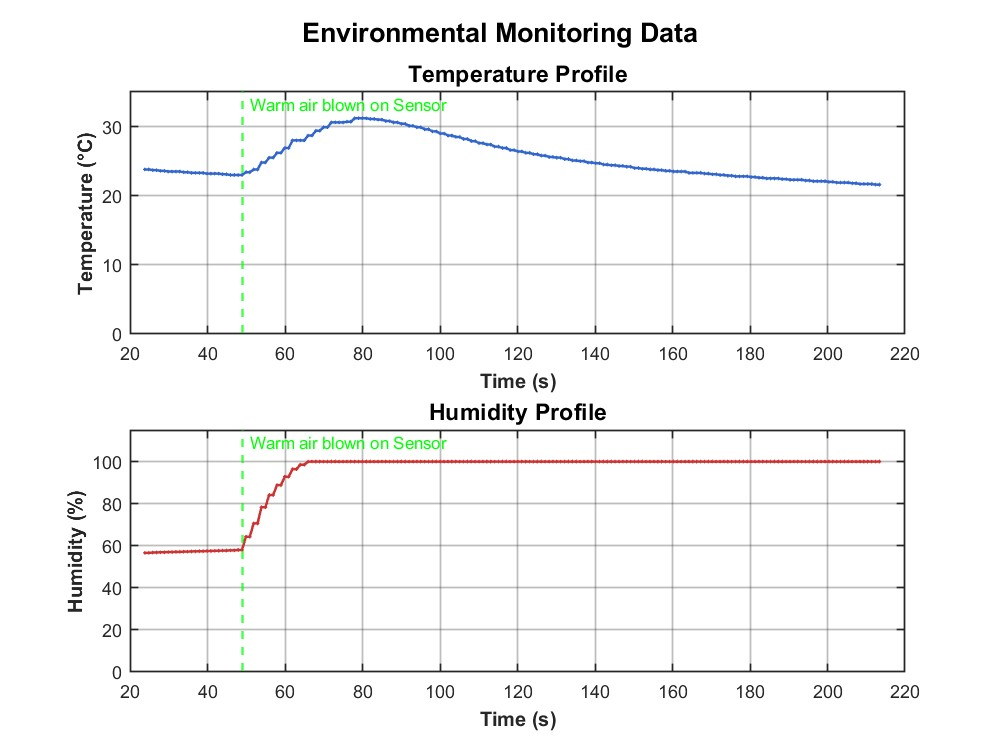
\includegraphics[width=0.7\textwidth]{figs/dthtest.jpg}
	\caption{DHT22 response to applied warm air (temperature and humidity vs. time).}
	\label{fig:dht22_test}
\end{figure}

\subsubsection*{Discussion}
The test confirms that the DHT22 sensor responds promptly to changes in environmental conditions, with smooth and continuous data output. 
The test showed the expected rise in both temperature and humidity. 
However, it was noted that the humidity readings temporarily saturated at the maximum percentage due to condensation forming within the sensor. 
After a short period, the values gradually returned to ambient levels. 
While this behavior is not ideal, it is a known characteristic of the sensor under extreme conditions and is not expected to cause issues during normal greenhouse operation, where such rapid condensation is unlikely to occur. 
Slight response delays were also noted, which are consistent with the DHT22's documented sampling rate and latency.

\subsection{Summary of Additional Sensor Tests}

Following the same testing approach described above, all sensors were validated for responsiveness and reliability. 
Each test involved controlled exposure to changing environmental conditions, with data recorded via serial communication and analyzed in MATLAB. 
A summary of key results is provided below, as the procedures followed were identical to those of the DHT22 test.

\subsubsection*{Soil Moisture Sensor}
The sensor was connected to the ESP32 microcontroller through ADC and real‑time values were logged. The sensor probes were sequentially tested in open air, damp soil, and fully submerged conditions. 
As shown in Figure~\ref{fig:soilmoisture_test}, the readings ranged from approximately \(0\%\) in dry air to \(80\%\) when submerged, demonstrating clear distinction between soil moisture states. 
The sensor provided consistent and repeatable readings, confirming its suitability for automated irrigation control. The calibration process will ensure more accurate mapping of percentage values to volumetric water content, but the results demonstrate strong baseline performance for the intended application.

\begin{figure}[H]
	\centering
	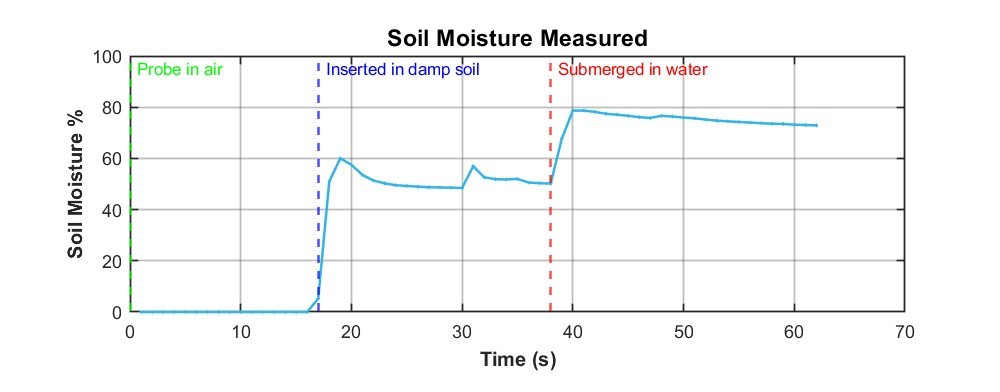
\includegraphics[width=0.8\textwidth]{figs/soiltest.jpg}
	\caption{Soil moisture sensor response in open air, damp soil, and submerged in water.}
	\label{fig:soilmoisture_test}
\end{figure}

\subsubsection*{Light Sensor}
The BH1750 light sensor was connected to the ESP32 via the I2C interface, and its lux readings were logged in real time. The sensor was exposed to varying illumination using a handheld torch. 
As seen in Figure~\ref{fig:bh1750_test}, the sensor responded sharply, rising from 40\,lux (ambient) to approximately 200\,lux under direct illumination, then returning to baseline upon removal of the light source. 
This confirmed its accuracy and responsiveness to dynamic lighting conditions. 

\begin{figure}[H]
	\centering
	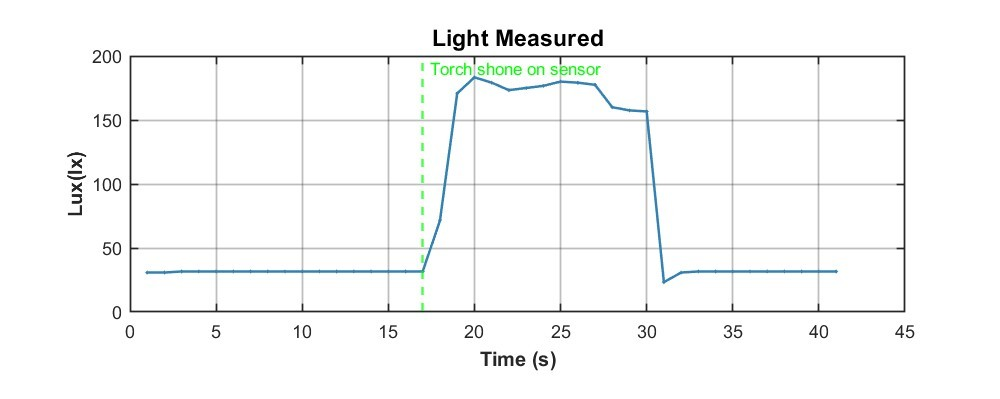
\includegraphics[width=0.7\textwidth]{figs/lighttest2.jpg}
	\caption{BH1750 light sensor response to torch illumination and return to ambient lighting.}
	\label{fig:bh1750_test}
\end{figure}

\subsubsection*{CO\textsubscript{2} Sensor}
The MHZ19B CO\textsubscript{2} sensor was connected to the ESP32 via UART communication and its readings were logged in real time. The sensors readings were allowed to stabilize at ambient indoor conditions (approximately 1000\,ppm) before being exposed to a burst of exhaled air. 
The concentration rapidly increased to the sensor’s limit of 5000\,ppm, then decayed back to baseline within two minutes, as shown in Figure~\ref{fig:co2_response}. 
This validated the sensor’s sensitivity, recovery time, and overall suitability for environmental monitoring.

\begin{figure}[H]
	\centering
	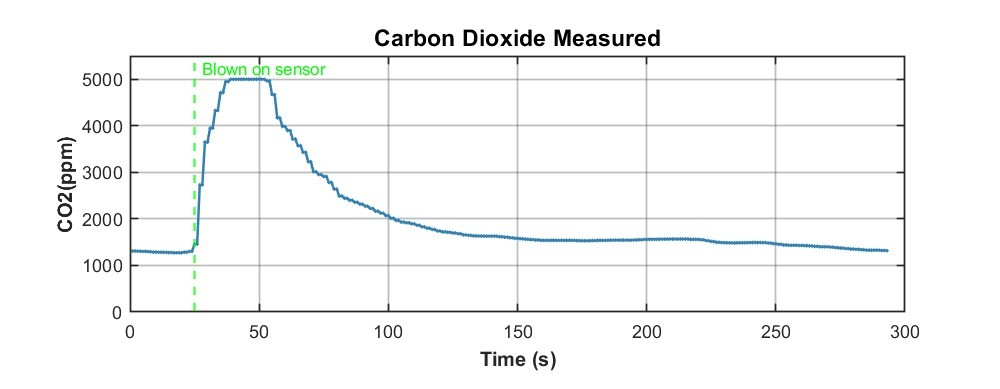
\includegraphics[width=0.7\textwidth]{figs/CO2test.jpg}
	\caption{CO\textsubscript{2} sensor response to rapid change in concentration.}
	\label{fig:co2_response}
\end{figure}

\subsection*{Summary Discussion}
Across all tests, the sensors exhibited expected and reliable responses to environmental variations. 
Minor latency and saturation effects observed under extreme conditions are consistent with manufacturer specifications and are not expected to affect normal operation. 
The results confirm that all selected sensors are well-suited for integration into the automated greenhouse control system.

\section{Actuator Validation }

Each actuator was connected to its respective relay channel, corresponding to the assigned GPIO pin on the microcontroller. 
Testing was carried out by first supplying the rated voltage directly to each actuator, followed by validation through relay control. 
A logical HIGH signal was written to each GPIO pin to trigger the relay, with successful activation confirmed visually via the built-in indicator LED and audibly by the distinct clicking sound of the relay switch. 
As the relay module operates in active-high mode, actuators were connected to either the Normally Open (NO) or Normally Closed (NC) terminals as required. 
Once verified, the appropriate 5\,V or 12\,V supply was connected to the Common (CO) port to power the actuators. 
Table~\ref{tab:actuator_tests} summarizes the testing procedures and outcomes for each actuator.

\begin{table}[H]
	\centering
	\caption{Actuator Testing and Observations}
	\label{tab:actuator_tests}
	\begin{tabular}{|p{3cm}|p{6cm}|p{6cm}|}
		\hline
		\textbf{Actuator} & \textbf{Test Procedure} & \textbf{Observation} \\
		\hline
		Solenoid Valve & 12\,V applied directly, then via relay control. Bulk and high-frequency capacitors added to suppress voltage spikes. & Audible switching confirmed; misting nozzles activated and deactivated with relay control. \\
		\hline
		Linear Actuator & 12\,V applied with polarity switching, then via relay-controlled H-bridge. & Extension and retraction observed correctly in both directions. Relay control verified reliable actuation. \\
		\hline
		Supplemental Lighting & 12\,V applied directly, then switched via relay control. & Purple UV grow light switched on and off reliably under both direct and relay control. \\
		\hline
		Intake / HAF Fans & 12\,V applied directly, then via relay control. & Fans powered on successfully; airflow observed. Relay switching confirmed proper operation. \\
		\hline
	\end{tabular}
\end{table}

With the mains water supply connected, the solenoid valve successfully controlled the misting system, providing adequate pressure to the misting nozzles. The nozzles were observed to start and stop spraying water in direct response to the relay switching.

During testing, it was observed that switching the misting solenoid simultaneously with Wi-Fi activity (e.g., ThingSpeak uploads) introduced supply transients that caused the ESP32 to briefly brown-out and reset. The solenoid’s inductive kickback and relay contact bounce injected noise onto the 12 V rail, which coupled into the 5 V supply. To mitigate this, a bulk electrolytic capacitor and a high-frequency ceramic capacitor were added at the solenoid driver terminals. These components damped the transient response and provided local energy buffering, resulting in stable system operation without timeouts or resets.

\section{Remote monitoring}

\subsection{Objective}
The objective of this experiment was to verify the successful implementation of remote monitoring and user control for the greenhouse system. The aim was to confirm that environmental parameters could be measured, transmitted, stored, and visualized in real time through wireless platforms, and that user-defined setpoints could be remotely updated.

\subsection{Methodology}
The test was conducted using the ESP32 microcontroller configured to interface with two IoT platforms: \textit{ThingSpeak} and \textit{Blynk}.  
For remote monitoring, the ESP32 was programmed to upload data for all environmental parameters including temperature, humidity, soil moisture, CO\textsubscript{2}, and light intensity at 20-second intervals to the ThingSpeak cloud platform. A custom dashboard was developed to visualize these readings in real time, as shown in Figure~\ref{fig:Wireless Monitoring Dashboard}.  

For remote control, the system was integrated with the Blynk IoT platform. A mobile dashboard was created (Figure~\ref{fig:Blynk}) to enable the user to adjust key control parameters such as temperature and humidity setpoints through sliders and buttons. . The ESP32 was connected to Eduroam services and configured with a unique
Blynk template and authentication token, allowing remote updates of setpoints for various environmental parameters.

\subsection{Results}
The greenhouse successfully transmitted all sensor data to ThingSpeak without communication interruptions. The online dashboard updated at the programmed 20-second interval, confirming the reliability of wireless data transfer and cloud visualization. Historical data was logged and plotted on the ThingSpeak channel, verifying successful storage for later analysis, as presented in Section~\ref{sec:response}.

\begin{figure}[H]
	\centering
	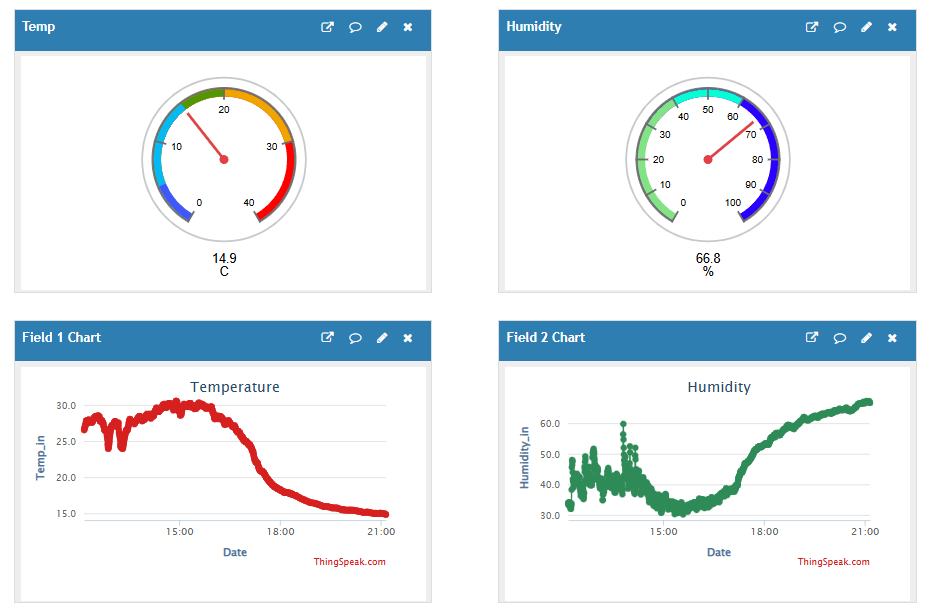
\includegraphics[width=0.7\textwidth]{figs/dash.png}
	\caption{Wireless Monitoring Dashboard.}
	\label{fig:Wireless Monitoring Dashboard}
\end{figure}


The Blynk dashboard enabled real-time modification of environmental setpoints from a mobile device. Commands sent via Blynk were received by the microcontroller with negligible delay. Parameter changes were reflected in the system's behaviour, demonstrating successful two-way communication between the user and the greenhouse.

\begin{figure}[H]
	\centering
	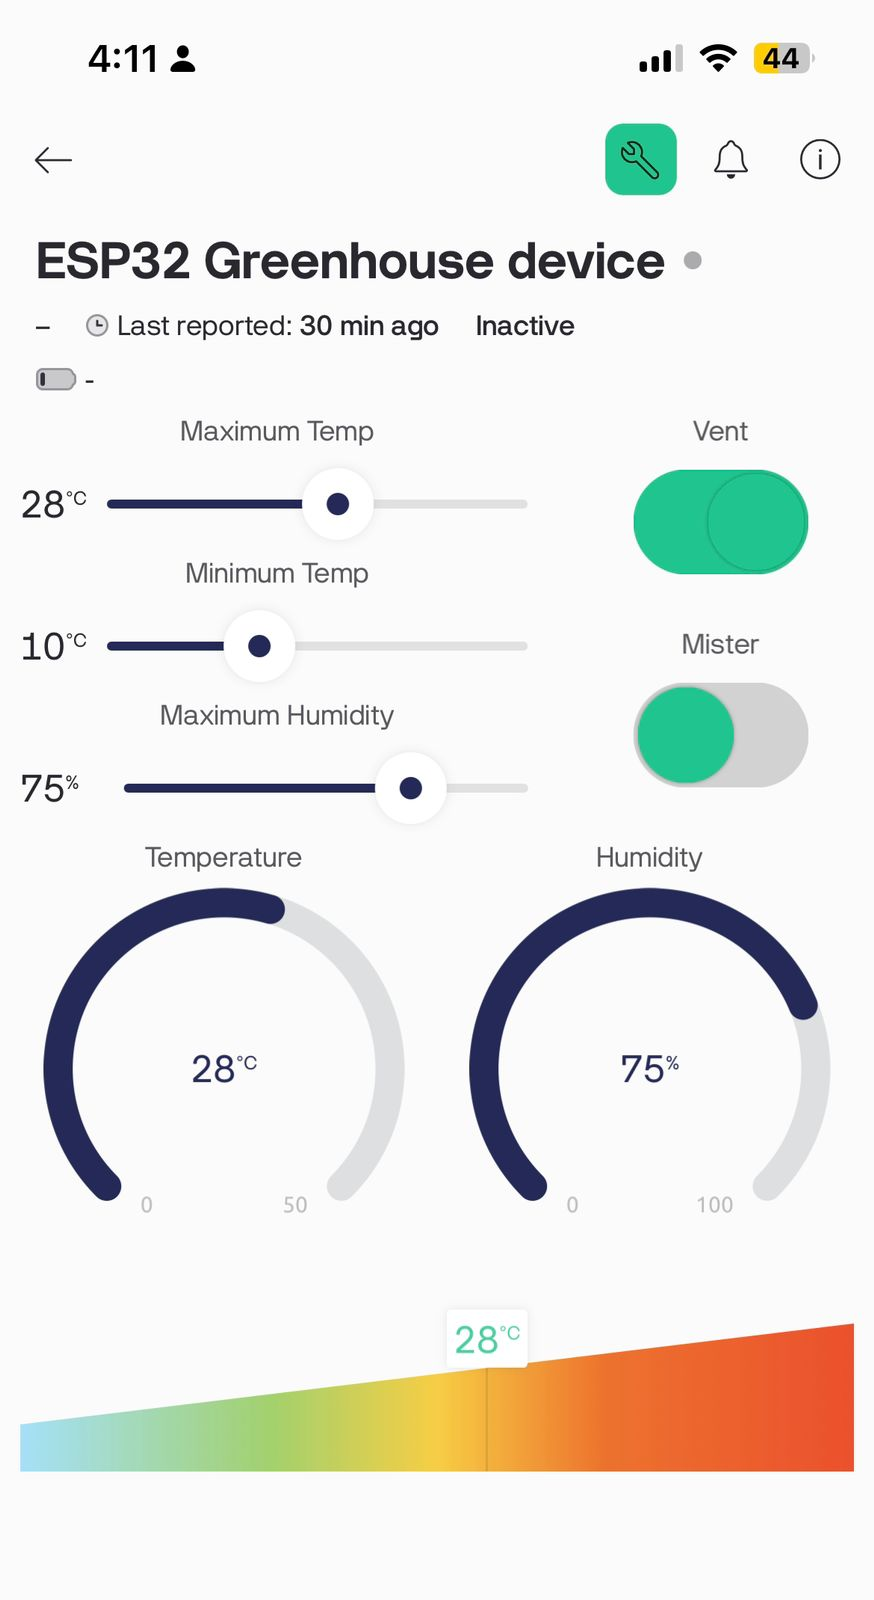
\includegraphics[width=0.35\textwidth]{figs/blynk.jpeg}
	\caption{User App with Blynk}
	\label{fig:Blynk}
\end{figure}


\subsection{Discussion}
The experiment confirmed that both remote data monitoring and user interaction were successfully achieved. While ThingSpeak proved effective for real-time data visualization and long-term data storage, Blynk offered a more intuitive interface for real-time control adjustments. The combined use of these platforms allows both analytical monitoring and interactive management of greenhouse conditions.


\section{Solar Power Test}

To validate the capability of the solar subsystem to power the greenhouse entirely off-grid, a series of tests were conducted. The procedure was as follows:

\begin{enumerate}
	\item The battery voltage was measured with no load connected, showing 12.8\,V, indicating a partial state of charge (full charge is approximately 14.8\,V).  
	\item The battery was connected to the Skyking charge controller via the positive and negative terminals. Upon connection, the controller powered on and displayed the battery voltage.  
	\item Using the controller menu, the float voltage was set to 13.7\,V, the discharge stop voltage to 10.8\,V, and the battery type configured as a sealed gel battery, in accordance with the battery manufacturer’s recommended operating conditions.  
	\item The solar panels were connected using MC4 connectors. The charge controller confirmed successful charging through its display.  
	\item The 12\,V supply terminal block and greenhouse system ground were connected to the load terminals of the charge controller.  
	\item The controller display indicated power transfer to the load. This was verified by measuring the potential difference across the load terminals with a multimeter.  
\end{enumerate}

These steps confirmed correct wiring and successful operation of the solar power subsystem. The charge controller additionally provides low-voltage protection by disconnecting the load if the battery voltage drops below a safe threshold. During full system testing, it was confirmed that the solar array supplied sufficient power to operate the greenhouse without discharging the battery to unsafe levels even during days with high cloud cover.


\section{Greenhouse Setup}

The Full Greenhouse setup can be seen in the figure below. Please see Appendix \ref{chap:pics} for additional pictures.

\begin{figure}[H]
	\centering
	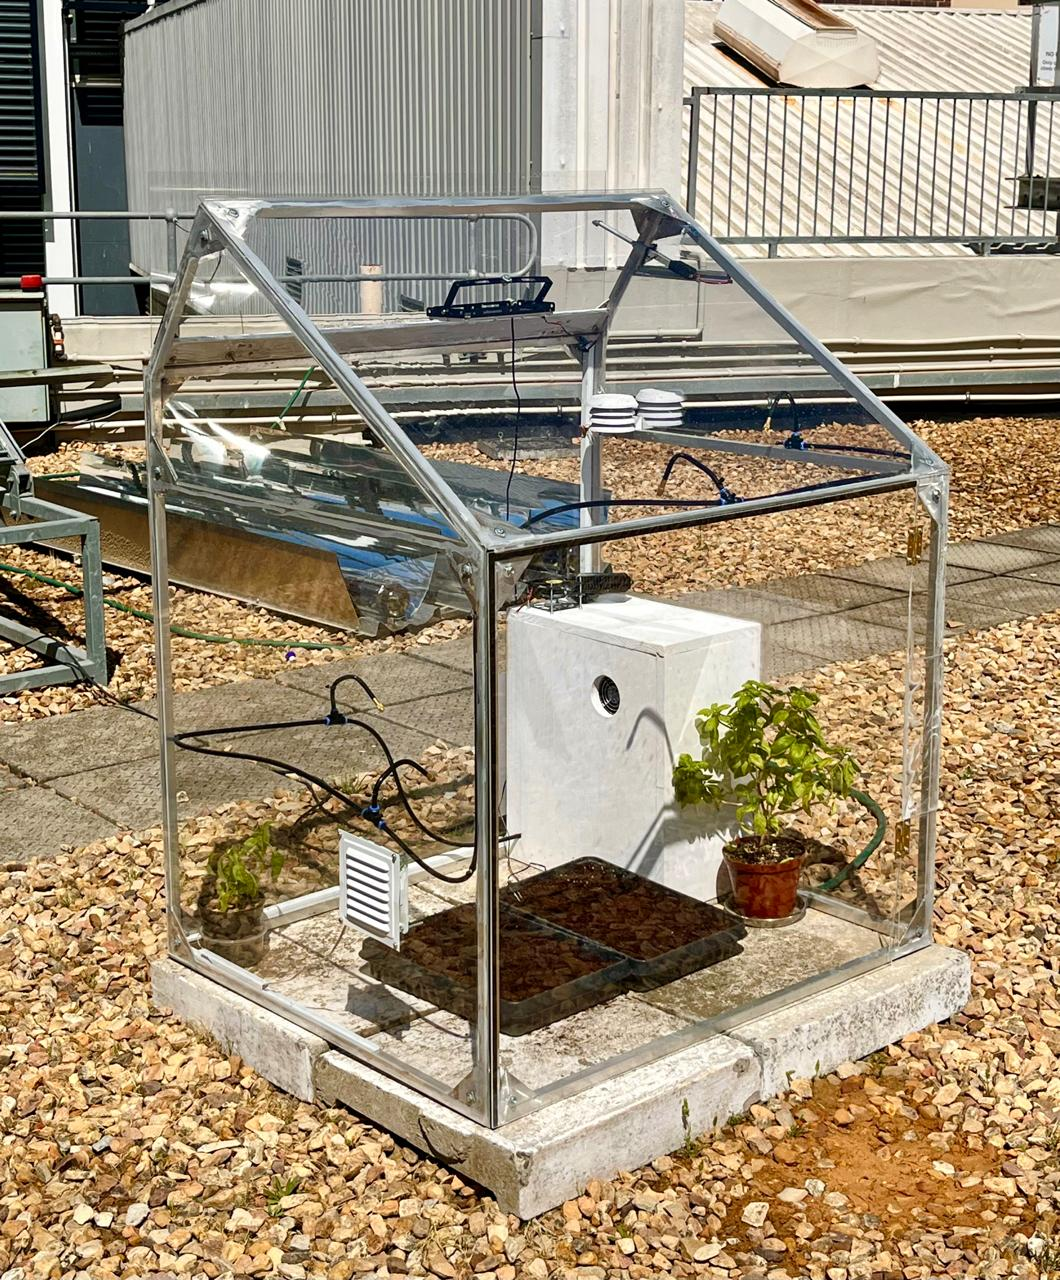
\includegraphics[width=0.4\textwidth]{figs/setup.jpeg}
	\caption{Greenhouse Setup}
	\label{fig:Greenhouse Setup}
\end{figure}

\section{Enviromental Response}\label{sec:response}

With all sensors, actuators, solar power components, and monitoring systems successfully tested, installed, and integrated, the complete greenhouse system can now be operated with all functions active. The system is powered on and allowed to continuously measure environmental conditions while autonomously regulating the internal climate toward the desired setpoints.

\subsection{ Dual Phase Test}

To evaluate the performance of the greenhouse control system, a two-phase test procedure was conducted. In the first phase, the greenhouse was operated for three full day–night cycles with all sensors and monitoring systems active, but without the actuators connected. This allowed the internal environment to respond passively to external conditions, providing a baseline measurement of natural fluctuations in temperature, humidity, and light.

In the second phase, the actuators (ventilation, irrigation, and heating) were connected and enabled. The greenhouse was again run for more than three full day–night cycles, with the control system actively attempting to regulate conditions towards the desirable setpoints. This phase demonstrates the effectiveness of the system in stabilizing the greenhouse environment.

The temperature, humidity and soil data from both phases were collected from Thingspeak and plotted using python, enabling a direct comparison between passive response and active control. The resulting figures highlight the extent to which the actuators improve environmental stability and overall system performance.

\begin{figure}[H]
	\centering
	\begin{subfigure}[b]{0.7\textwidth}
		\centering
		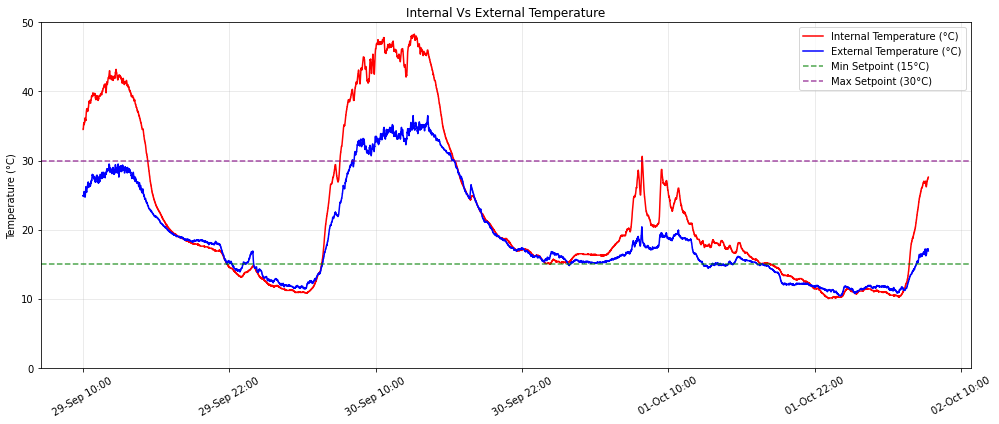
\includegraphics[width=\textwidth]{figs/temp_n.png}
		\caption{Actuators off}
		\label{fig:temp_off}
	\end{subfigure}
	\vskip\baselineskip
	\begin{subfigure}[b]{0.7\textwidth}
		\centering
		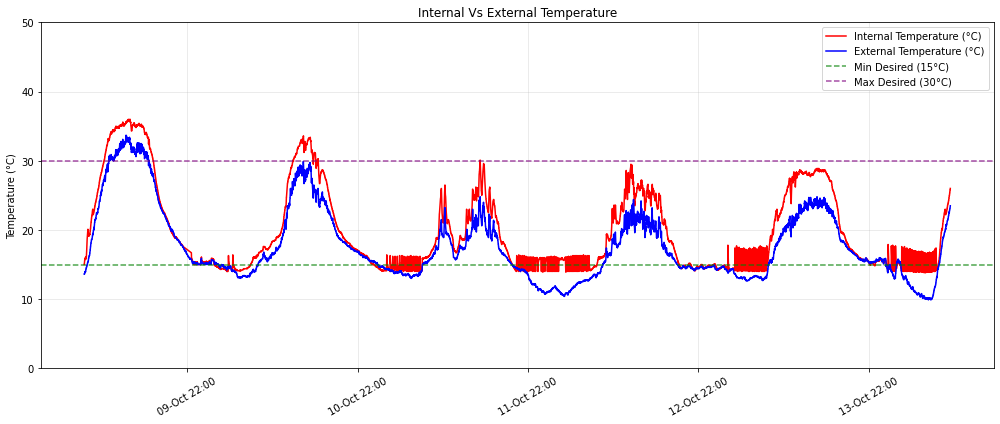
\includegraphics[width=\textwidth]{figs/temp_a.png}
		\caption{Actuators on}
		\label{fig:temp_on}
	\end{subfigure}
	\caption{Internal vs. external temperature profiles for the greenhouse with (a) Actuators off and (b) Actuators on.}
	\label{fig:temp_comparison}
\end{figure}


During the actuator-off test, the internal environment of the greenhouse was allowed to fluctuate naturally with ambient conditions. Without any active control, the internal temperature (shown in red) rose to a peak of approximately \SI{48}{\celsius} during the day, significantly exceeding optimal growing conditions. At night, the temperature dropped well below the desired setpoint, reaching approximately \SI{10}{\celsius}, highlighting the system’s vulnerability to external temperature extremes under passive operation.

In contrast, during the actuator-on test, the greenhouse exhibited an improved thermal response. The heating system successfully maintained the internal temperature near the desired setpoint of \SI{15}{\celsius} during cooler periods, keeping the environment consistently warmer than outside conditions. However, under hot daytime conditions, the system faced challenges in reducing internal temperatures, which remained around \SI{5}{\celsius} above ambient. Despite this limitation, the active ventilation, circulation fans, and misting system provided measurable cooling benefits compared to the uncontrolled scenario, in which temperatures rose to approximately \SI{15}{\celsius} above ambient due to the unchecked greenhouse effect heating the internal environment.

\begin{figure}[H]
	\centering
	\begin{subfigure}[b]{0.7\textwidth}
		\centering
		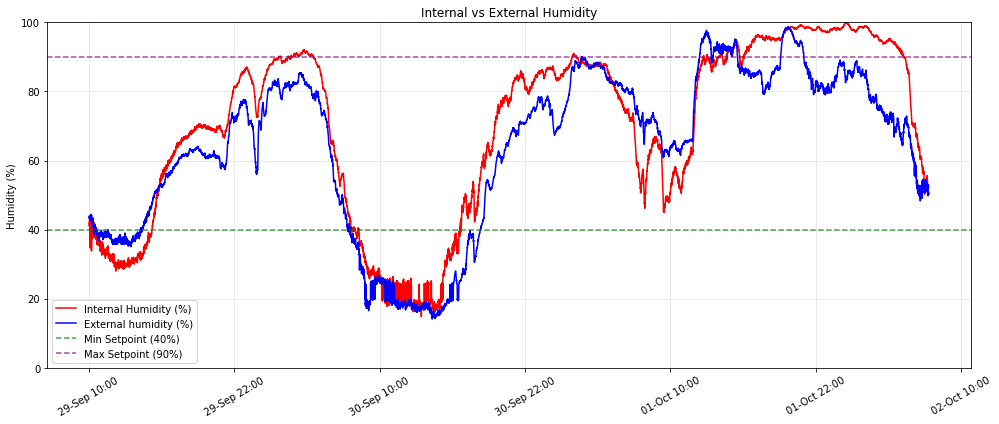
\includegraphics[width=\textwidth]{figs/hum_n.png}
		\caption{Actuators off}
		\label{fig:hum_off}
	\end{subfigure}
	\vskip\baselineskip
	\begin{subfigure}[b]{0.7\textwidth}
		\centering
		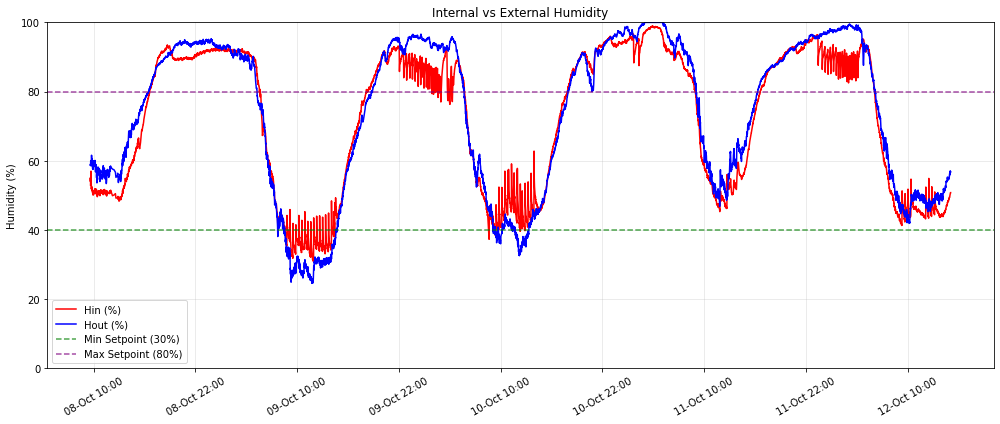
\includegraphics[width=\textwidth]{figs/hum_a.png}
		\caption{Actuators on}
		\label{fig:hum_on}
	\end{subfigure}
	\caption{Internal vs.\ external humidity profiles for the greenhouse with (a) actuators off and (b) actuators on.}
	\label{fig:hum_comparison}
\end{figure}


During the actuator-off phase, the internal and external humidity profiles closely mirrored one another, with relative humidity varying widely between 20\% and 100\% over the day–night cycle. This variation reflects the natural dependence of relative humidity on temperature, decreasing during the warmer daytime periods and increasing overnight.

When the actuators were enabled, the system responded to low humidity by activating the misting function every 20 minutes, visible as periodic spikes in the recorded data. These misting periods effectively restored the internal humidity to within the desired range, demonstrating successful environmental regulation. At night, operation of the heater caused a further decrease in humidity, an unintended but beneficial effect that prevented excessive condensation and maintained more balanced conditions during peak humidity levels. However, during times when the heater was inactive due to adequate internal temperatures, the humidity occasionally exceeded the desired maximum setpoint. 

Overall, the actuator-on phase exhibited a more stable humidity range of 40\% to 100\%, compared to the uncontrolled 20\% to 100\% range. While the system was unable to maintain the desired maximum humidity limit of 90\%, it successfully prevented humidity from dropping below 40\%, demonstrating effective intermittent misting control.

\begin{figure}[H]
	\centering
	\begin{subfigure}[b]{0.7\textwidth}
		\centering
		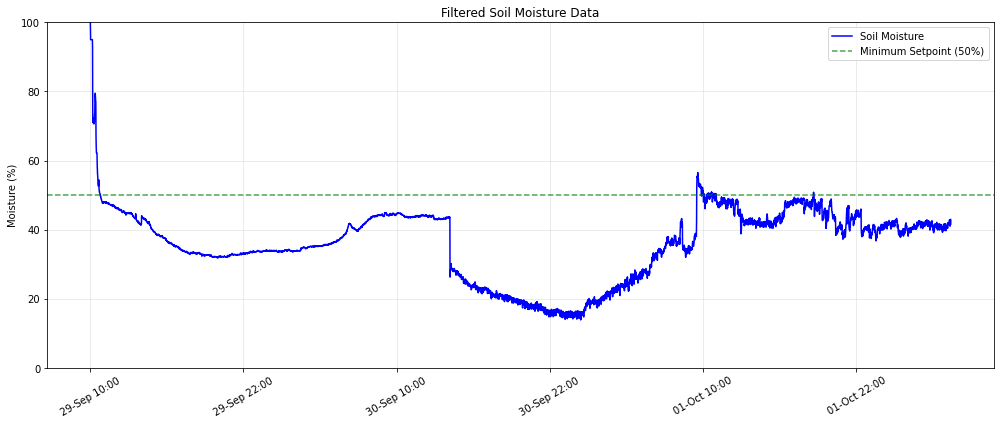
\includegraphics[width=\textwidth]{figs/soil_n.png}
		\caption{Actuators off}
		\label{fig:Soil_off}
	\end{subfigure}
	\vskip\baselineskip
	\begin{subfigure}[b]{0.7\textwidth}
		\centering
		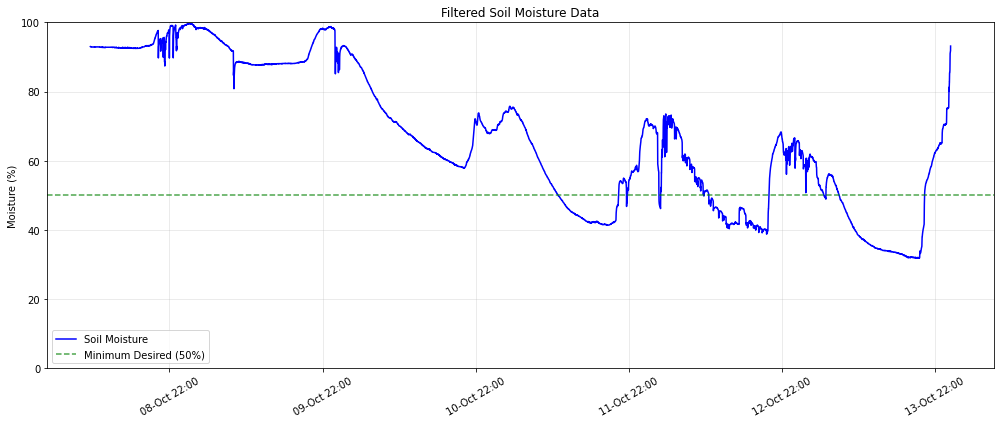
\includegraphics[width=\textwidth]{figs/soil_a.png}
		\caption{Actuators on}
		\label{fig:Soil_on}
	\end{subfigure}
	\caption{Soil Moisture profile for the greenhouse with (a) actuators off and (b) actuators on.}
	\label{fig:soil_comparison}
\end{figure}

During the initial phase, when the mister was inactive, the soil moisture content gradually declined and remained below the setpoint as the soil medium dried out. A slight increase was observed on the third day following a cold, rainy night, likely due to condensation re-entering the soil system.

When the actuators were enabled, the soil moisture stabilized around 70\% for several days before dropping below the setpoint, at which point the misting system activated to restore the desired moisture level. The data showed a recurring pattern of moisture loss during the night, followed by misting events during the day that raised levels above the setpoint. On average, the system maintained soil moisture within or slightly above the desired range, demonstrating effective control based on sensor feedback.

The fluctuations and response delays observed, are attributed to the misting system’s operational settings, restricted to daytime activation and governed by a duty cycle of two minutes on every twenty minutes, as described in Appendix~\ref{flow}. These constraints were intentionally implemented to prevent overwatering, allow time for sensor feedback stabilization, and avoid unintended nighttime cooling when thermal regulation takes priority.

\subsection{ CO\textsubscript{2} and Lux Observation}

\begin{figure}[H]
	\centering
	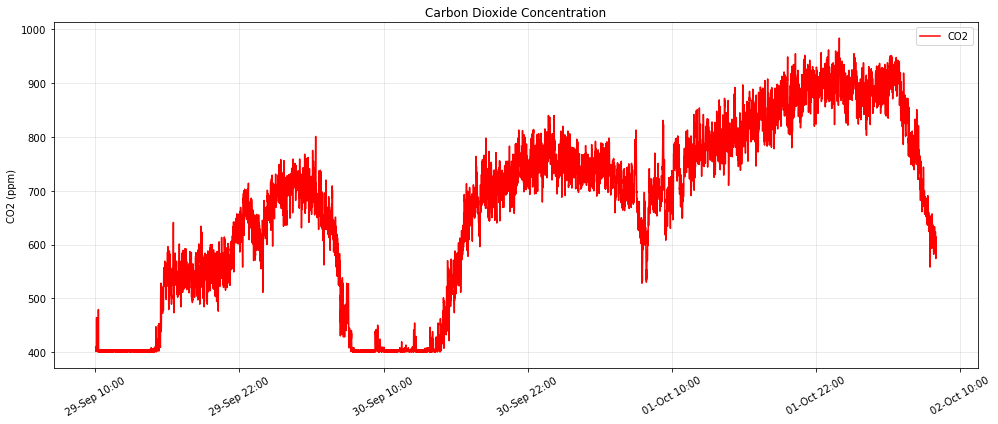
\includegraphics[width=0.7\textwidth]{figs/co2data.png}
	\caption{CO\textsubscript{2} Profile}
	\label{fig:CO2}
\end{figure}


The \(\mathrm{CO_{2}}\) plot provides valuable insight by highlighting a distinct day–night cycle, with concentrations rising during the night as a result of plant respiration. 
This trend is consistent with general ambient \(\mathrm{CO_{2}}\) behavior and does not indicate any problematic accumulation within the greenhouse. Since the levels remained within healthy ranges for plant growth, no active control or actuation was required, such as venting to regulate concentrations.  


\begin{figure}[H]
	\centering
	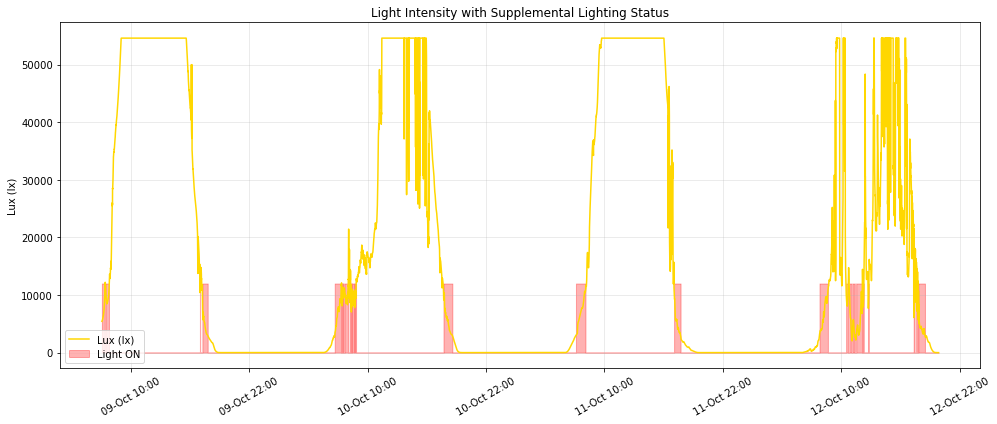
\includegraphics[width=0.7\textwidth]{figs/lux.png}
	\caption{Lux Profile}
	\label{fig:Lux}
\end{figure}

The plot of the light intensity profile illustrates the digital on/off state of the supplemental LED lighting. 
As calculated in Appendix~D, the LED was designed to provide 
\SI{200}{\micro\mole\per\square\meter\per\second} PPFD and was configured to activate whenever the ambient 
levels dropped below this threshold, but only during daylight hours. This corresponds to an illuminance of approximately 
\SI{10800}{lux}. The lighting can be observed switching on during the early morning and evening periods, as well as 
intermittently on the second day when cloud cover reduced incoming solar radiation.

\section{Evaluation Using Performance Requirements}

\begin{threeparttable}
	\caption{Performance Requirement Verification}\label{tab:performance_verification}
	\begin{tabular}{|p{1.5cm}|p{4.5cm}|c|p{3cm}|p{3cm}|}
		\hline
		\textbf{PR Number} & \textbf{Description} & \textbf{Target} & \textbf{Actual} & \textbf{Comment} \\
		\hline
		2 & Resist Wind speeds & 18.81\,kph & Not Tested & Validated through calculations \\
		\hline
		3 & Temperature sensing range & -10–50\,°C & -40–80\,°C & Passed \\
		\hline
		4 & Soil moisture sensing & 0–100\,\% & 0–100\,\%  & Passed \\
		\hline
		5 & Humidity sensing & 0–100\,RH\% & 0–100\,RH\%  & Passed \\
		\hline
		6 & CO\textsubscript{2} sensing range & 0–1000\,ppm & 0–5000\,ppm & Passed \\
		\hline
		7 & Light sensing & 0–600\,\si{\micro\mole\per\metre\squared\per\second} & 0–925\,\si{\micro\mole\per\metre\squared\per\second} & Passed \\
		\hline
		8 & Latency in displaying environmental conditions & <120\,s & $\sim$30\,s average & Passed \\
		\hline
		9 & Control temperature & 15 min–30 max\,°C & 15–35\,°C maintained & 15 min Passed - 30 max Failed \\
		\hline
		10 & Control soil moisture content & 50–100\,\% & 50–100\,\% maintained during day & Passed \\
		\hline
		11 & Control humidity & 40 min–90 max\,\% & 40–95\,\% maintained & 40 min Passed - 90 max Failed \\
		\hline
		12 & Supplemental lighting intensity & 200\,\si{\micro\mole\per\metre\squared\per\second} & Not tested & Validated through calculations \\
		\hline
		13 & Energy consumption & 0–1200\,Wh & 980\,Wh over 24\,h & Validated in calculations \\
		\hline
		14 & Battery storage capacity & >24\,h & Not Tested & Remained sufficiently charged through solar over cloudy periods \\
		\hline
	\end{tabular}
\end{threeparttable}


\section{Full system Test with Plants Growth}

The operational success of the greenhouse system was validated through a controlled two-week growth trial of microgreens, conducted to verify the system’s ability to maintain suitable environmental conditions for plant growth. The experiment served as a performance test against the design requirements related to temperature, humidity, and irrigation control. Four microgreen varieties (peas, radish, beetroot, and arugula) were planted within the greenhouse. As shown in the before-and-after photographs below, all varieties exhibited healthy germination and growth, confirming that the system effectively supported sustained plant development and met its intended functional objectives.

\begin{figure}[H]
	\centering
	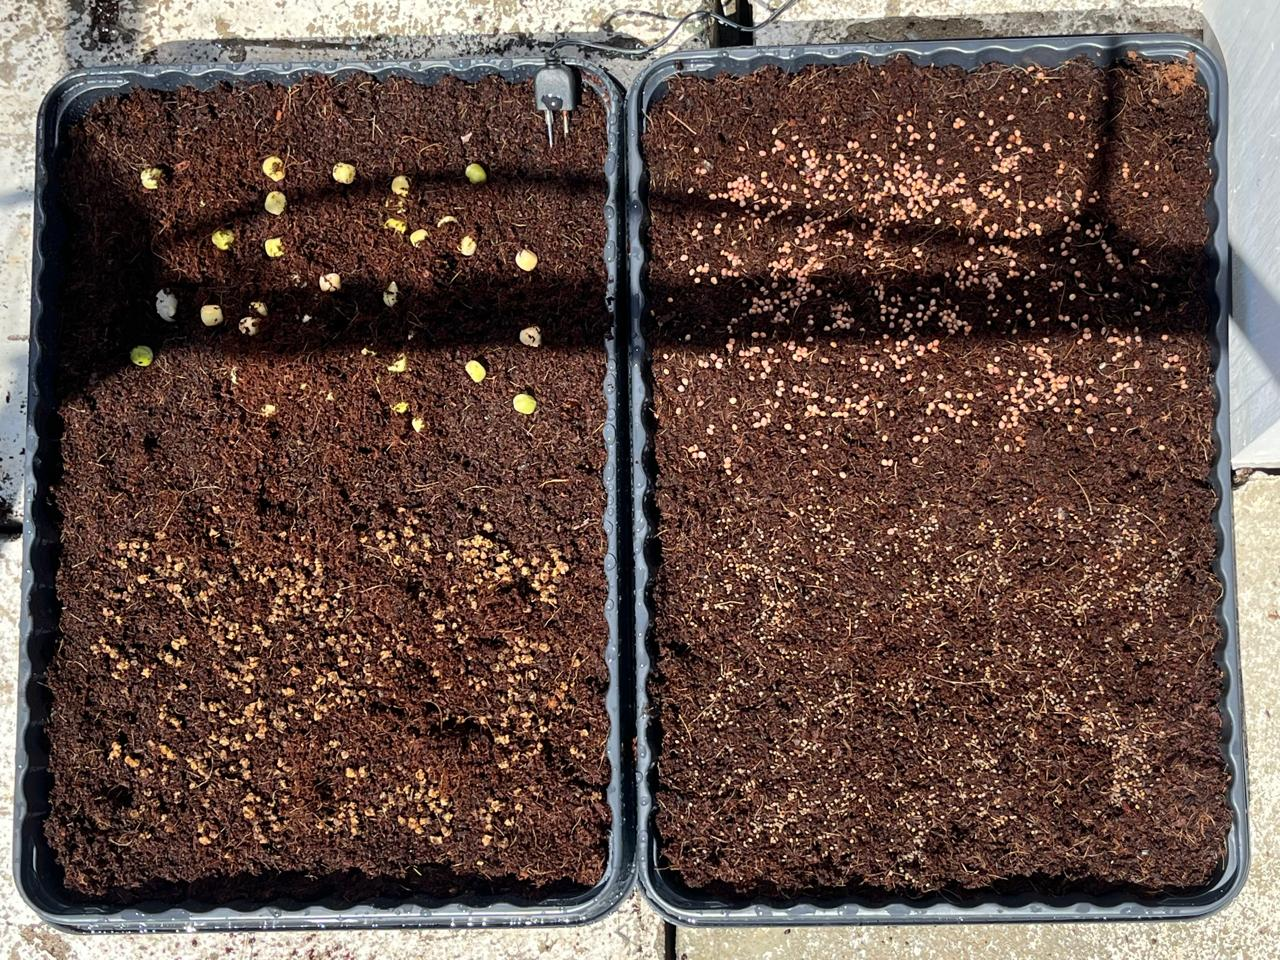
\includegraphics[width=0.7\textwidth]{figs/greens.jpeg}
	\caption{Microgreens Seeds}
	\label{fig:Microgreens}
\end{figure}

\begin{figure}[H]
	\centering
	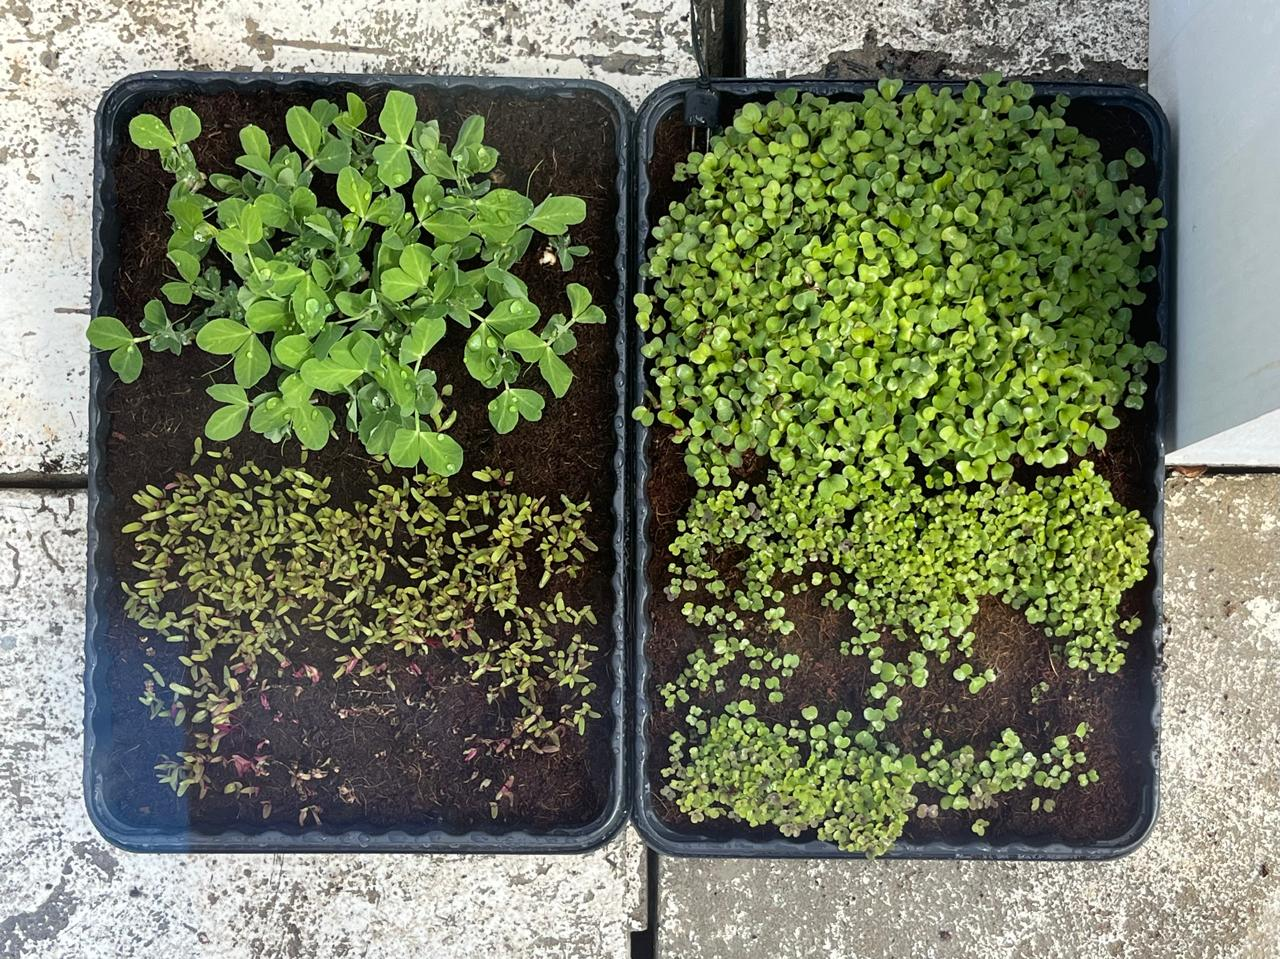
\includegraphics[width=0.7\textwidth]{figs/green2.jpeg}
	\caption{Microgreens}
	\label{fig:Microgreens}
\end{figure}


\chapter{Conclusions}

\section*{Future Reccomendations}

The results indicated that the design was effective in providing reliable monitoring of greenhouse conditions, as well as control of water supply, humidity, and supplemental lighting. However, the system showed limitations in its ability to regulate higher temperatures during hotter days. For future development of an automated greenhouse in the warmer climate of South Africa, alternative cooling strategies could be explored, such as motorized shading or the integration of an evaporative cooling pad. In addition, the sizing of intake and exhaust fans could be optimized with airflow capacity in mind, favoring an overcompensated design to ensure adequate ventilation under peak heat conditions.

\section*{Conclusions}

The design proved effective in monitoring all key parameters required to sustain healthy plant growth. Automated heating successfully maintained temperatures above the setpoint during cooler nights, while the misting system provided sufficient control of both humidity and water supply. 

The vent and intake fans contributed to improved airflow, helping to limit temperature rise compared to conditions without these actuators. Although overheating remained a challenge, the greenhouse system demonstrated the ability to regulate a microclimate capable of supporting plant life, while providing the user with real-time and historical data and control through the wireless dashboards.

In addition, the solar power system enabled fully off-grid operation, allowing the greenhouse to run entirely on renewable energy. This not only reduced the system’s carbon footprint but also highlighted its potential as a sustainable solution to address food insecurity by providing controlled growing conditions, with the primary limitation being high-temperature management.









\appendix%------------------------------------------

\renewcommand{\chaptername}{Appendix} % ensures "Appendix A"

\begin{appendices} % this sets headings like "Appendix A"
	\begin{landscape}
\chapter{Project Planning}

This appendix gives the estimated cost to complete the project in Figure A.2 and a Gantt chart for all the completed and planned activities in Figure A.1


\begin{sidewaysfigure}
	\centering
	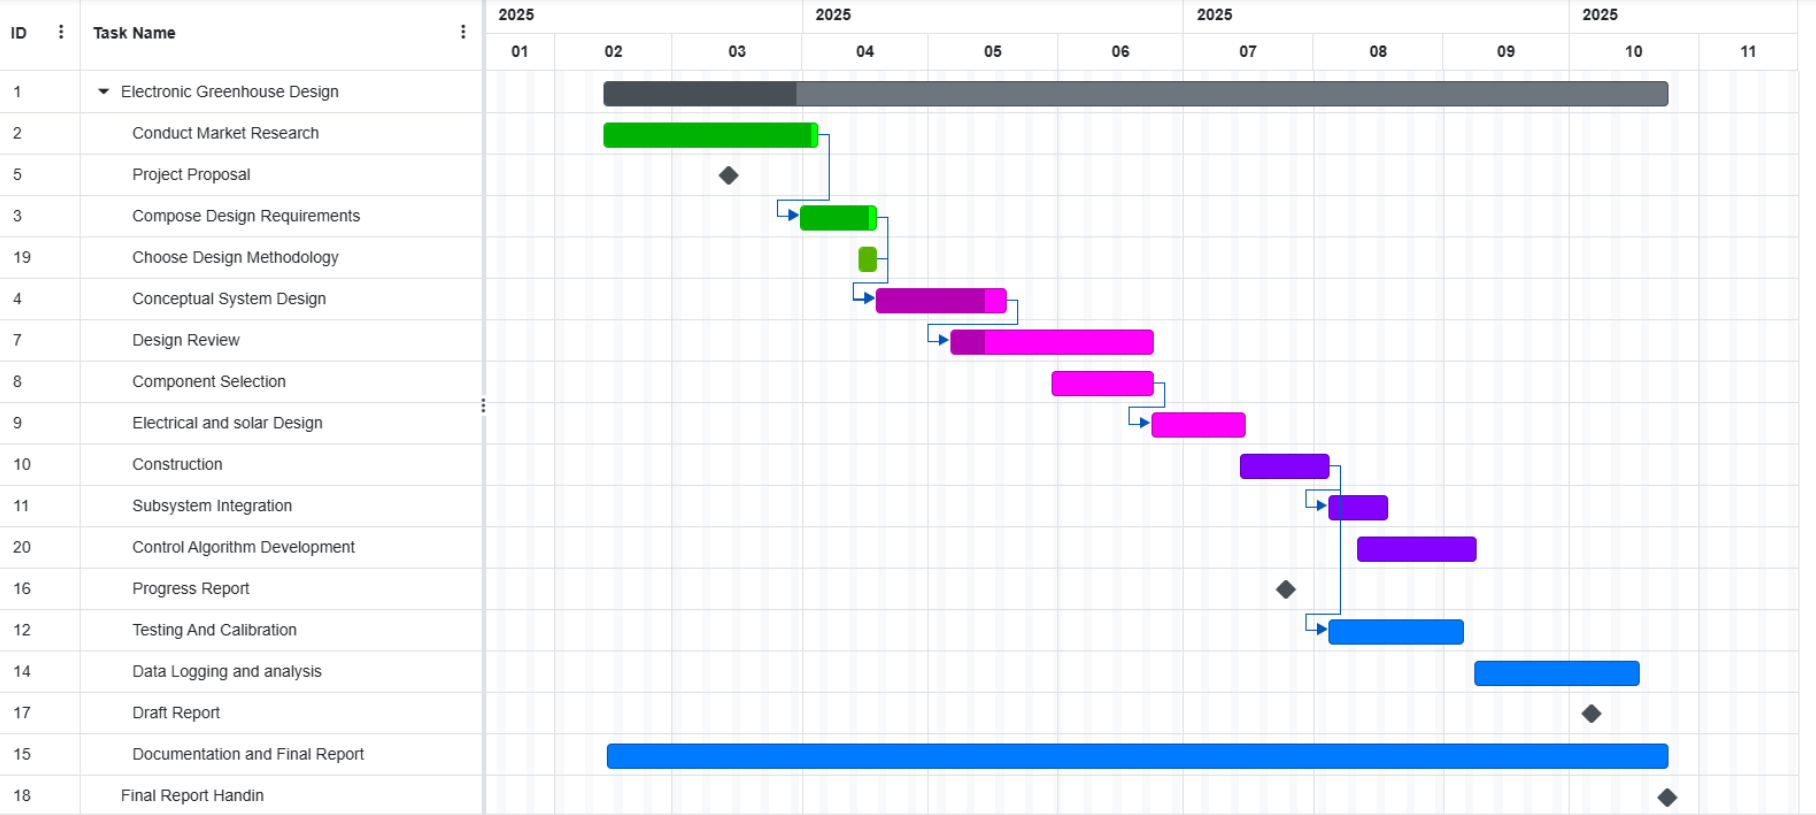
\includegraphics[width=1.3\textwidth]{figs/gant.png}
	\caption{Gantt Chart}
	\label{fig:Gant Chart}
\end{sidewaysfigure}

\end{landscape}


\begin{figure}[htbp]
    \centering
    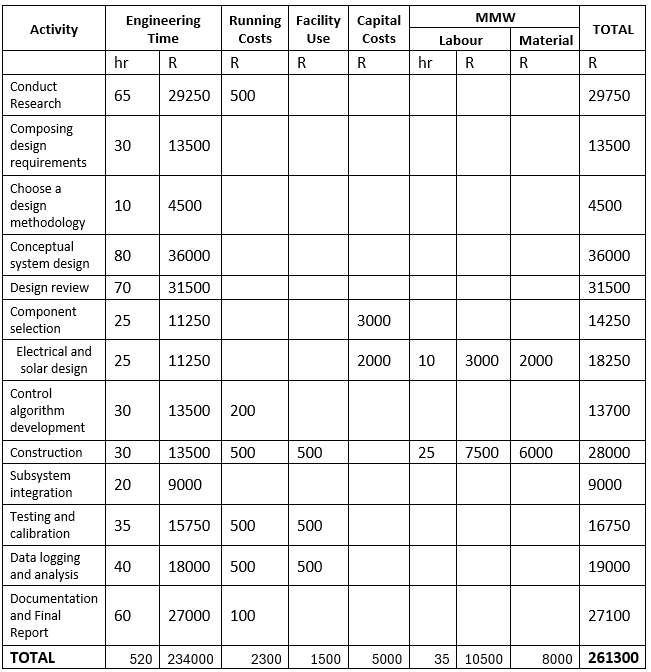
\includegraphics[width=1\textwidth]{figs/cost.png}
    \caption{Estimated Costs}
    \label{tab:Cost Estimate}
\end{figure}




	\chapter{Risk Analysis and Mitigation Procedures}
\begin{table}[H]
\footnotesize
\centering
\caption{Activity-Based Risk Assessment}
\begin{tabularx}{\textwidth}{|p{2.3cm}|X|p{1.1cm}|p{1cm}|X|}
\hline
\rowcolor[HTML]{EFEFEF}
\textbf{Activity} & \textbf{Risk} & \textbf{Risk Level} & \textbf{Risk Type} & \textbf{Mitigating Steps} \\
\hline
Navigating lab & Tripping on loose cable or equipment & Low & P/E & Don’t leave cables lying around \\
\hline
Work taking place on roof & Falling & Low & P & Use harness, avoid edges, complete heights training \\
\hline
Turning on/off equipment & Electric shock & Low & P & Check cables to ensure that insulation is intact, include warning signage \\
\hline
Use of hot glue gun & Accidentally contacting hot glue causing burn to skin & Medium & P & Wear protective gloves, ensure glue has enough time to cool before handling \\
\hline
Wiring of ports & Incorrect wiring may cause damage to components & Low & E & Make use of proper wiring diagram, label wires physically as laid out in diagram \\
\hline
Soldering connections of wires & Accidentally contact with the soldering iron can result in burns to the user or damage components & Medium & P/E & Keep a clean soldering workstation and use a solder stand. Turn off iron when not in use \\
\hline
Handling fluids near the system and operation of irrigation system & Spilling fluids can cause damage to electrical components & High & E & Do not bring fluids close to the system. Ensure irrigation system is sealed \\
\hline
Wiring of components & Electrical shock due to bad isolation of wires & Medium & P/E & Check all wires are well insulated before supplying power and ensure emergency stop is accessible. Include warning signage \\
\hline
Vent actuation & Hands in the way of moving parts causing potential small cut, bruise or pinch & Low & P & Keep hands clear of vent when operational \\
\hline
HAF/intake fan operation & Hands in the way of moving parts causing potential small cut, bruise or pinch & Low & P & Keep hands clear of fans when operational. Install safety mesh and coverings to prevent contact \\
\hline
\end{tabularx}
\end{table}

	\begin{landscape}
	\chapter{Engineering Drawing}
	\addcontentsline{toc}{chapter}{Engineering Drawing}
	
	\begin{{sidewaysfigure}}
		\centering
		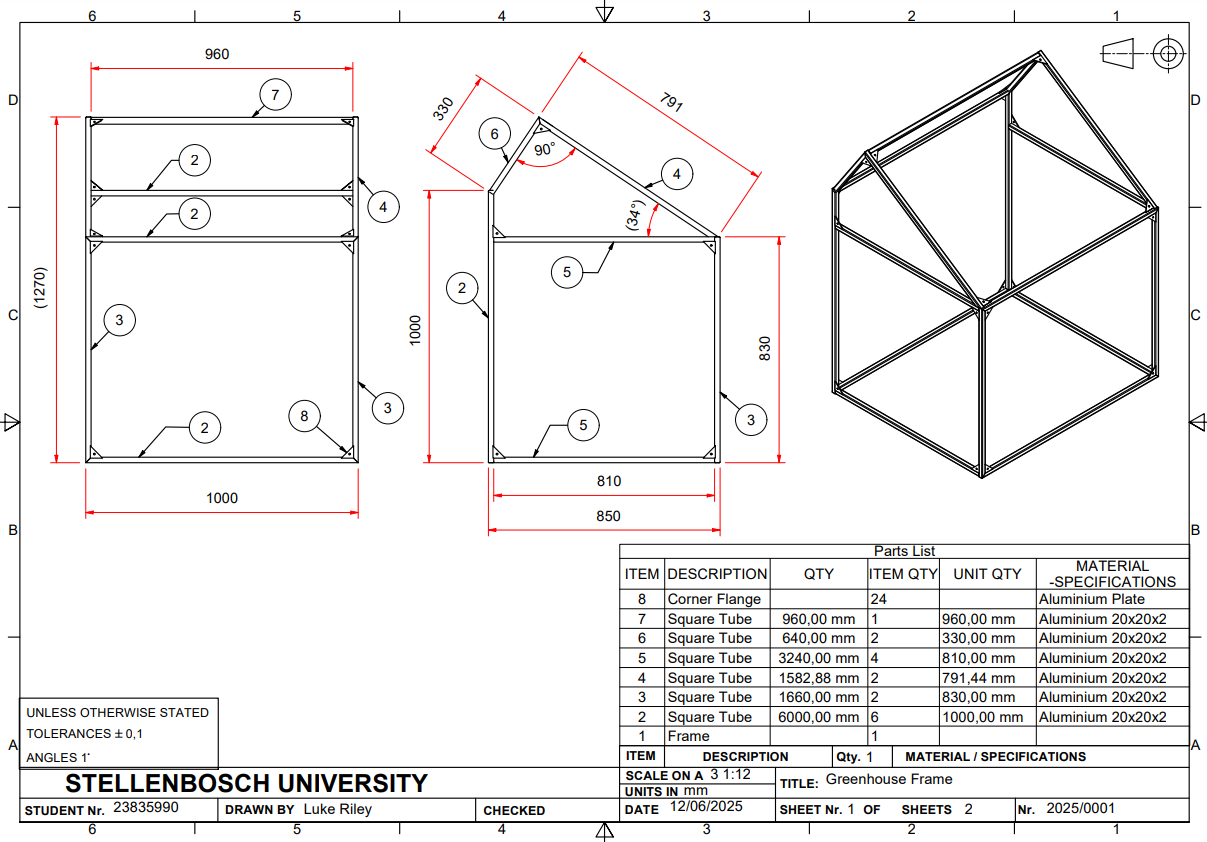
\includegraphics[width=0.8\linewidth]{figs/drawing.png}
		\caption{Engineering Drawing}
		\label{fig:engineering-drawing}
	\end{{sidewaysfigure}}
\end{landscape}
	\chapter{Calculations}

 \begin{figure}[H]
    \centering
    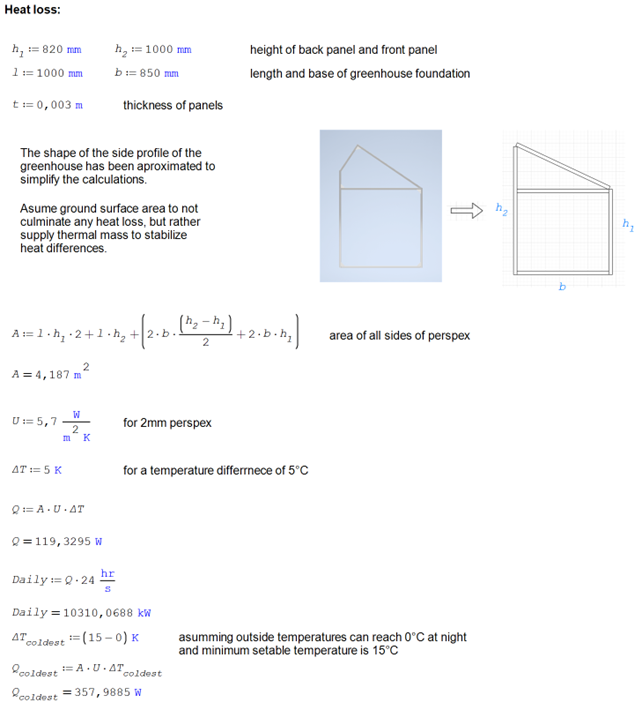
\includegraphics[width=1\textwidth]{figs/smath1.png}
\end{figure}

 \begin{figure}[H]
    \centering
    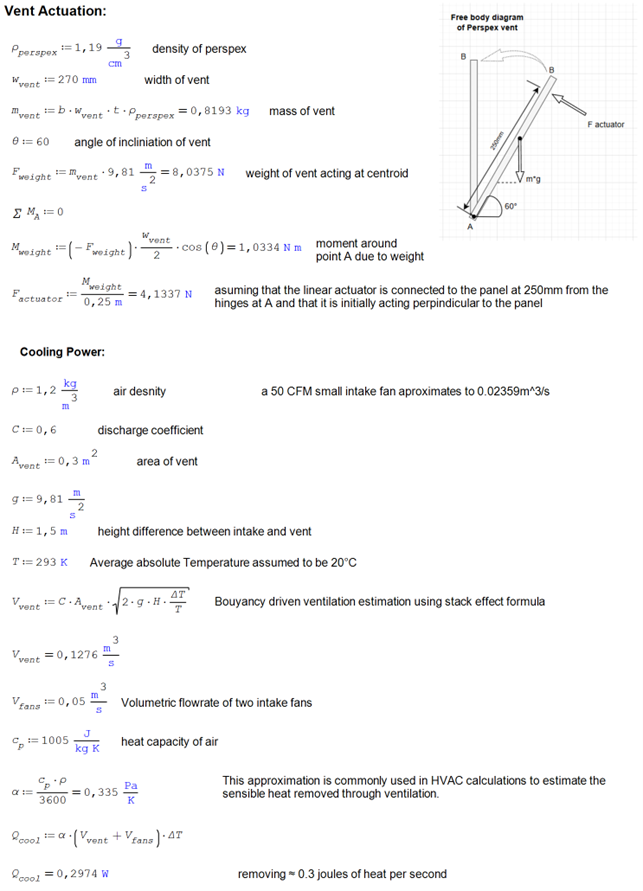
\includegraphics[width=1\textwidth]{figs/smath2.png}
\end{figure}
 \begin{figure}[H]
    \centering
    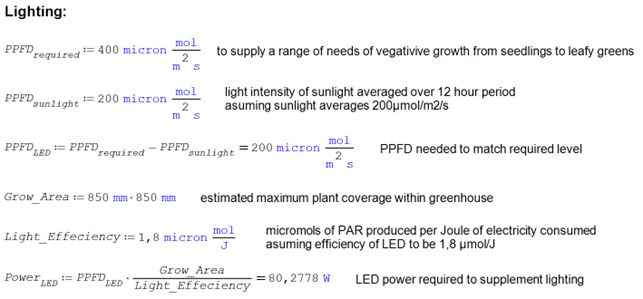
\includegraphics[width=1\textwidth]{figs/smath3.png}
\end{figure}
 \begin{figure}[H]
    \centering
    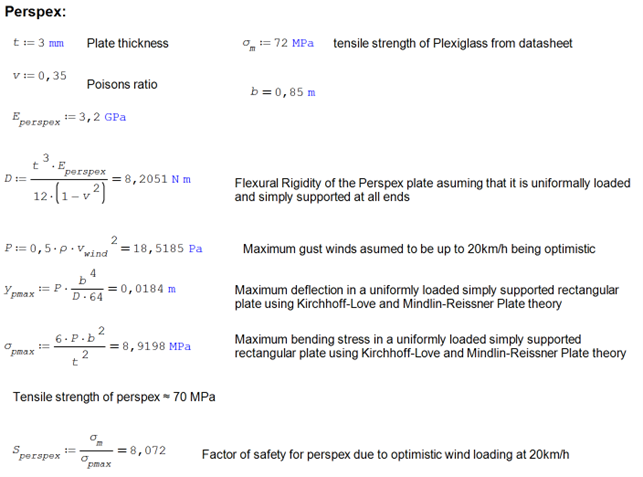
\includegraphics[width=1\textwidth]{figs/smath4.png}
\end{figure}
 \begin{figure}[H]
    \centering
    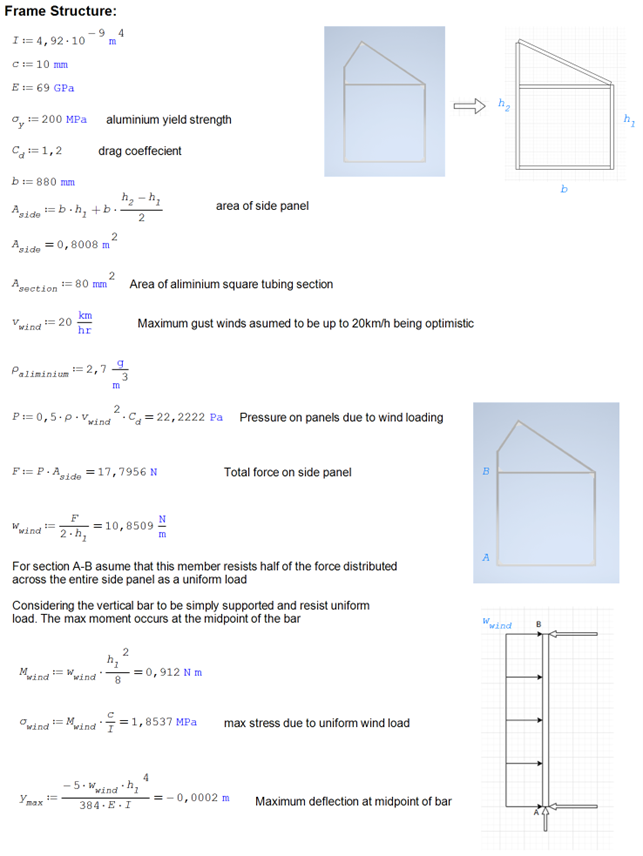
\includegraphics[width=1\textwidth]{figs/smath5.png}
\end{figure}
 \begin{figure}[H]
    \centering
    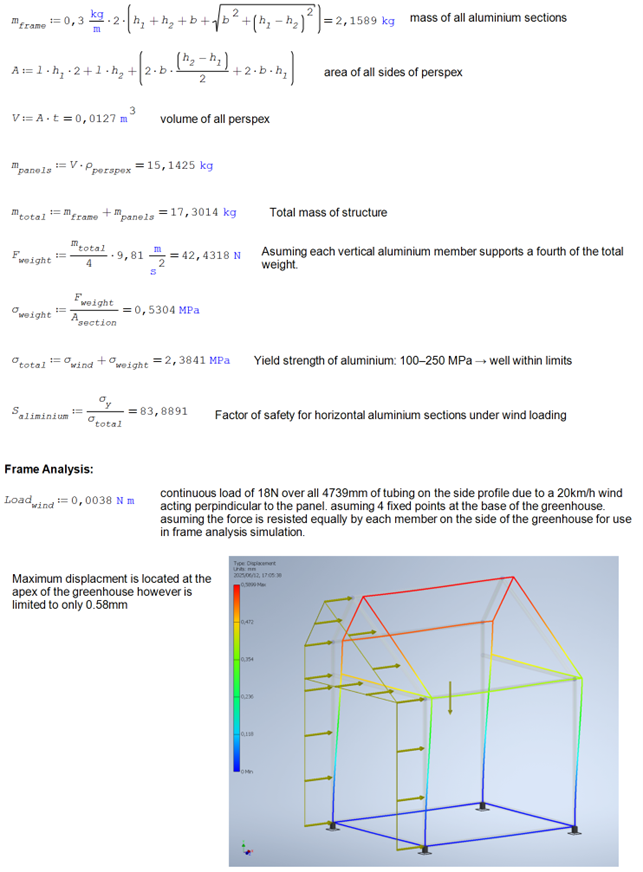
\includegraphics[width=1\textwidth]{figs/smath6.png}
\end{figure}
	% --- Setup Images appendix ---
\FloatBarrier
\chapter{Greenhouse Setup Images}\label{chap:pics}

\begin{figure}[H]  % was [p]
	\centering
	% First row
	\begin{subfigure}[b]{0.25\linewidth}
		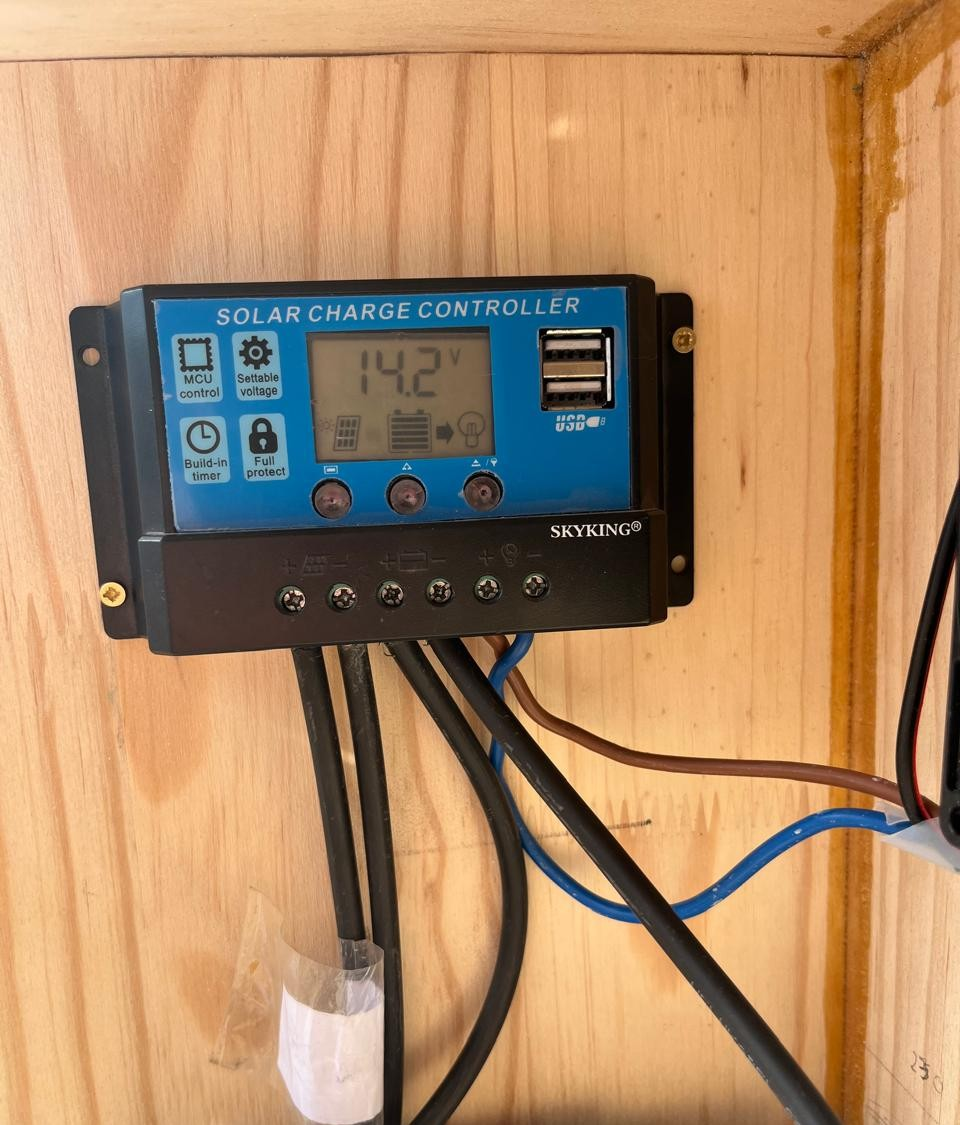
\includegraphics[width=\linewidth]{figs/mppt.jpeg}
		\caption{MPPT Controller}
		\label{fig:mppt}
	\end{subfigure}
	\begin{subfigure}[b]{0.25\linewidth}
		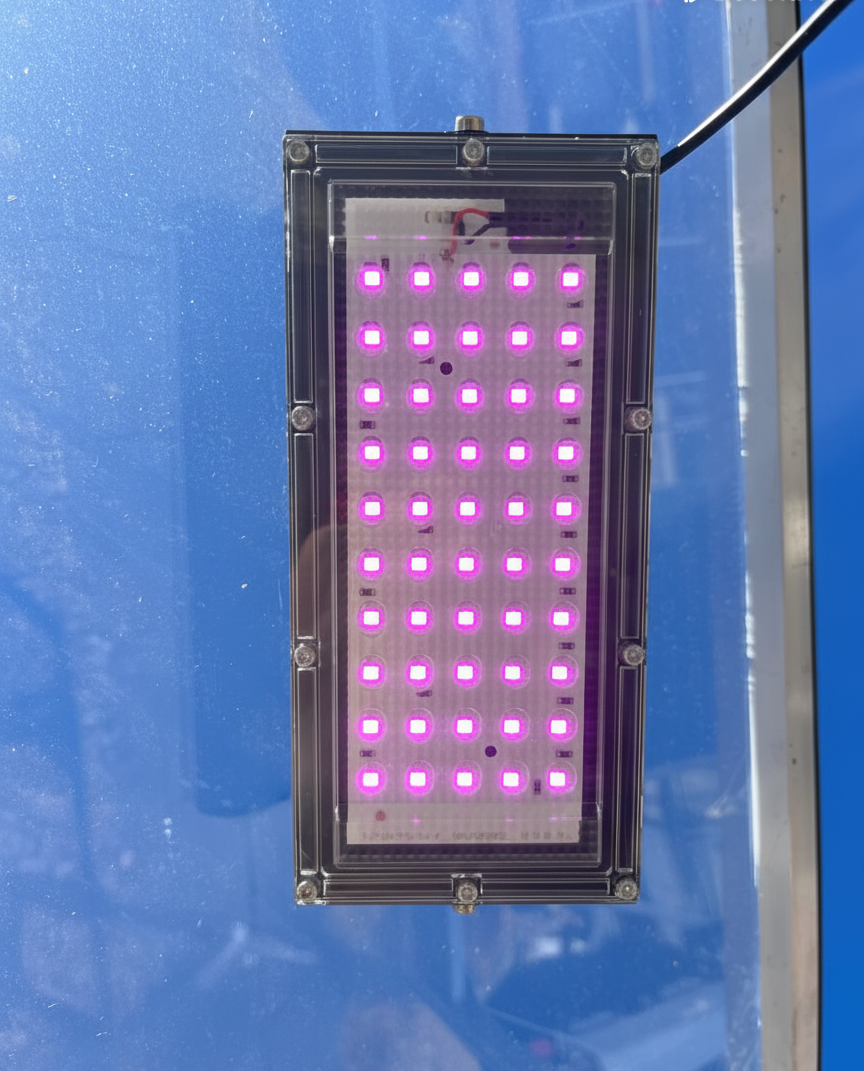
\includegraphics[width=\linewidth]{figs/LED.png}
		\caption{LED Lighting}
		\label{fig:led}
	\end{subfigure}
	\begin{subfigure}[b]{0.25\linewidth}
		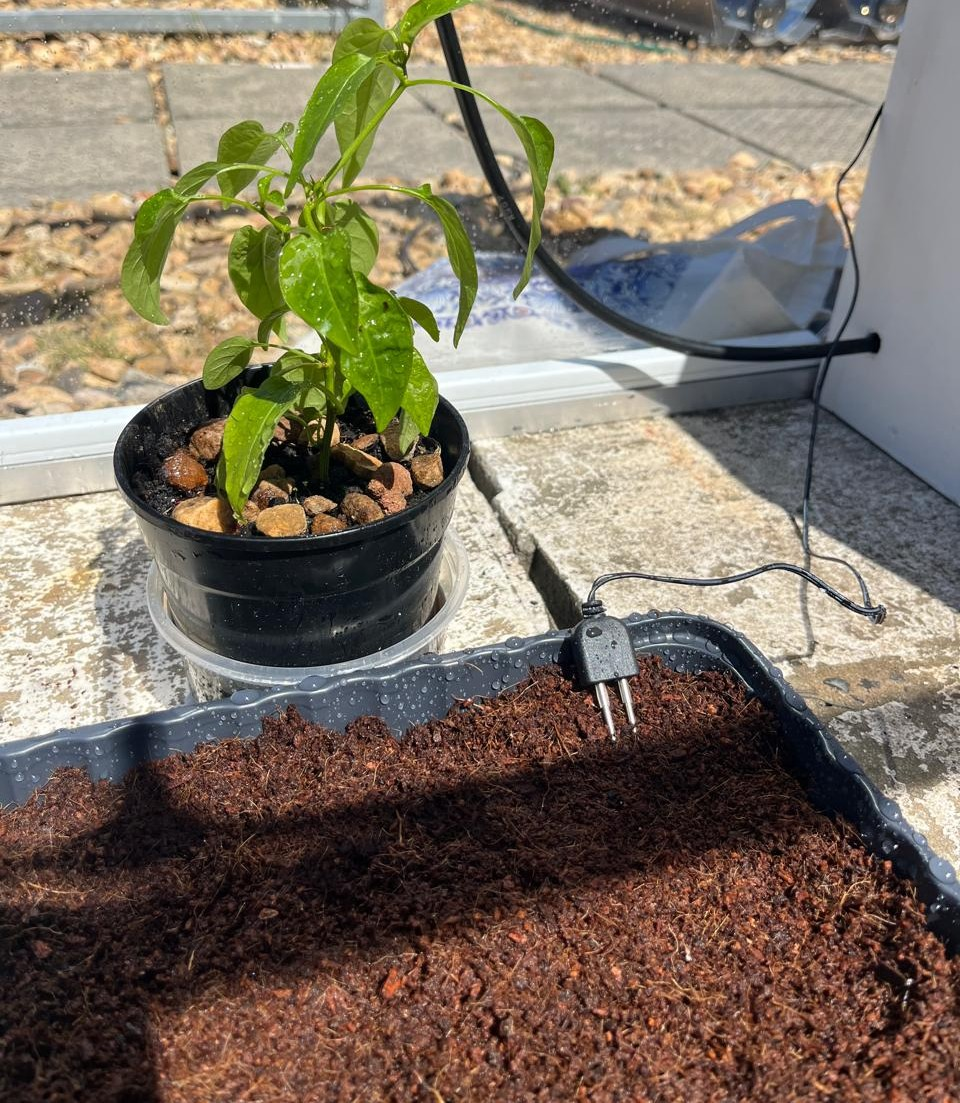
\includegraphics[width=\linewidth]{figs/soilsensor.jpeg}
		\caption{Soil Sensor}
		\label{fig:soil_sensor}
	\end{subfigure}
	
	% Second row
	\begin{subfigure}[b]{0.25\linewidth}
		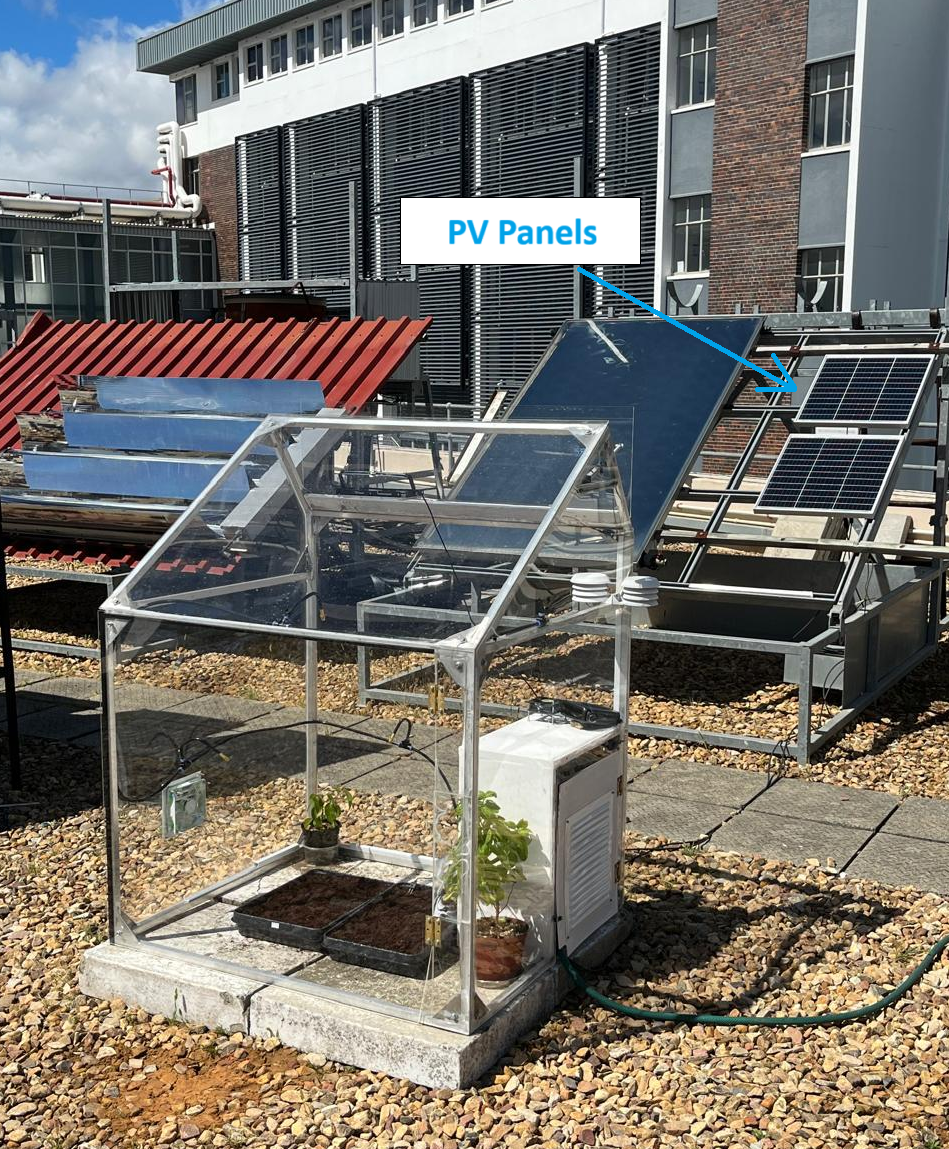
\includegraphics[width=\linewidth]{figs/pv.png}
		\caption{PV Panels}
		\label{fig:pv_panels}
	\end{subfigure}
	\begin{subfigure}[b]{0.25\linewidth}
		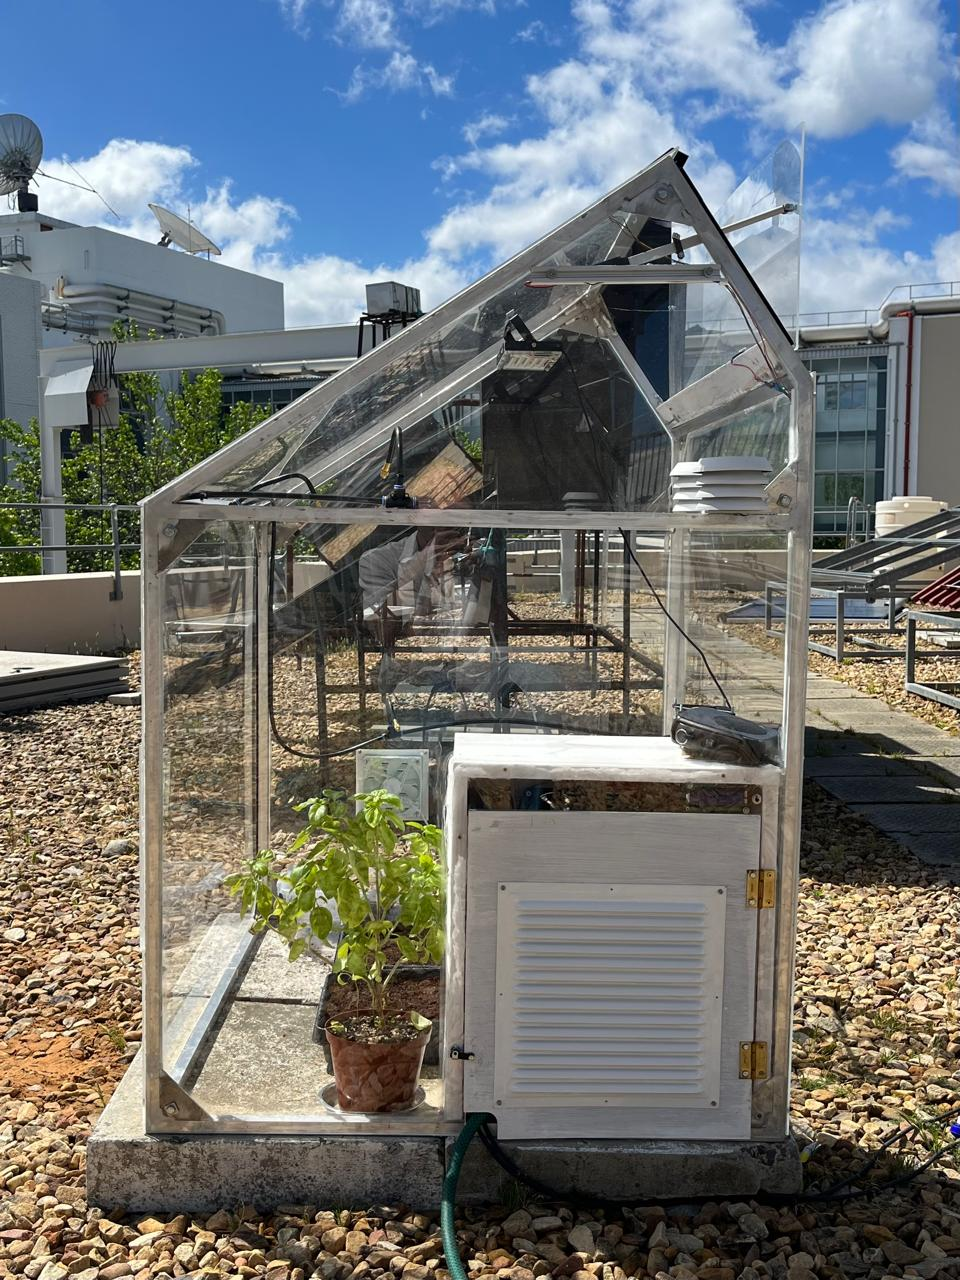
\includegraphics[width=\linewidth]{figs/Side.jpeg}
		\caption{Side profile with active vent}
		\label{fig:side_profile}
	\end{subfigure}
	\begin{subfigure}[b]{0.25\linewidth}
		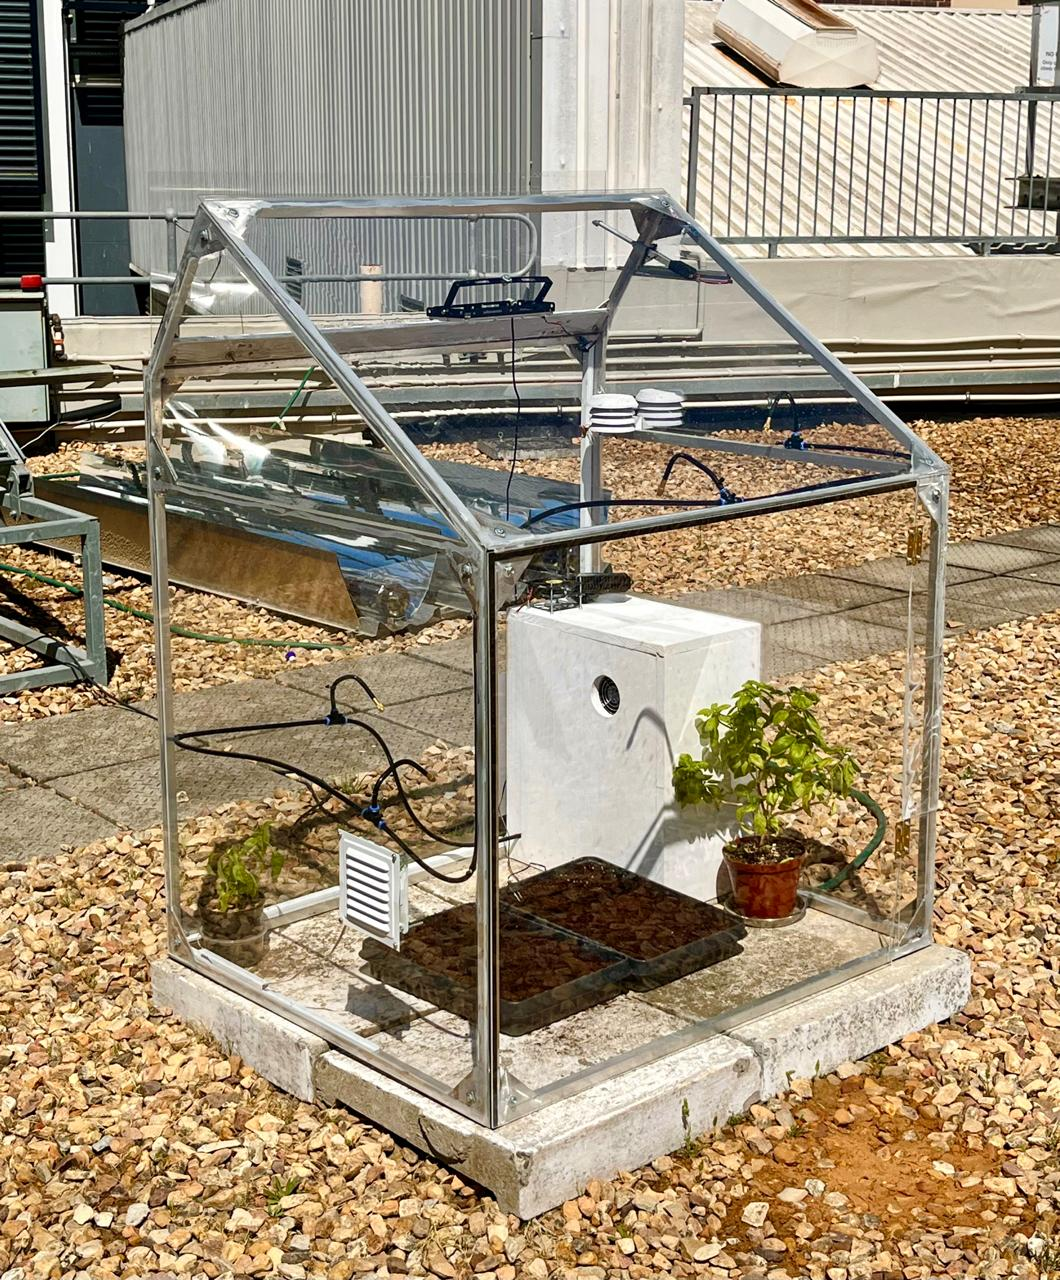
\includegraphics[width=\linewidth]{figs/setup.jpeg}
		\caption{Setup Overview}
		\label{fig:setup}
	\end{subfigure}
	
	% Third row
	\begin{subfigure}[b]{0.25\linewidth}
		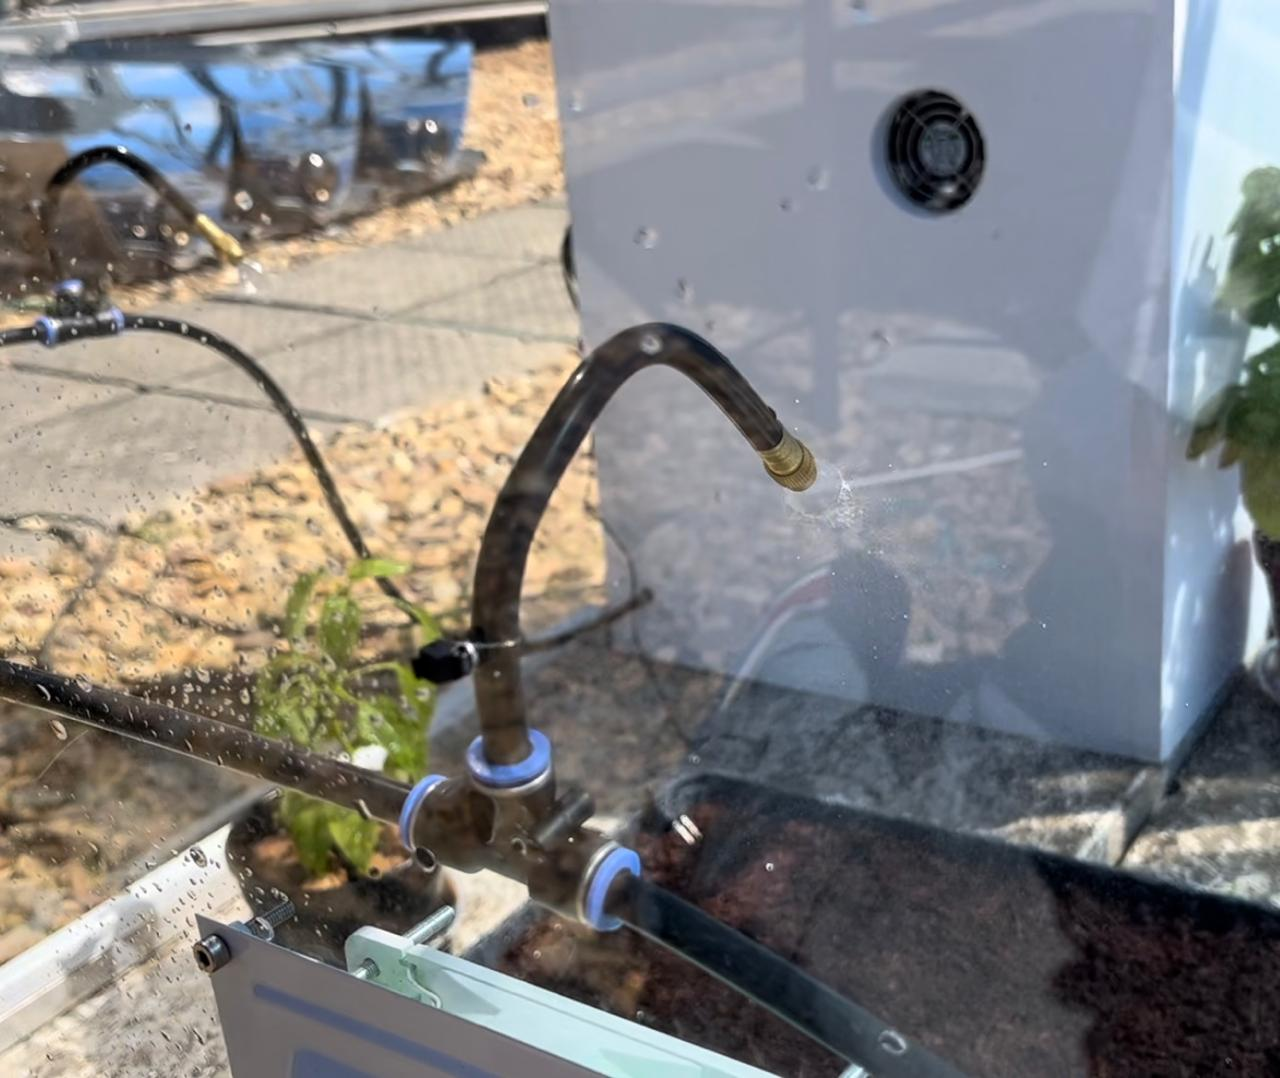
\includegraphics[width=\linewidth]{figs/mist.jpeg}
		\caption{Misting System}
		\label{fig:mist}
	\end{subfigure}
	\begin{subfigure}[b]{0.25\linewidth}
		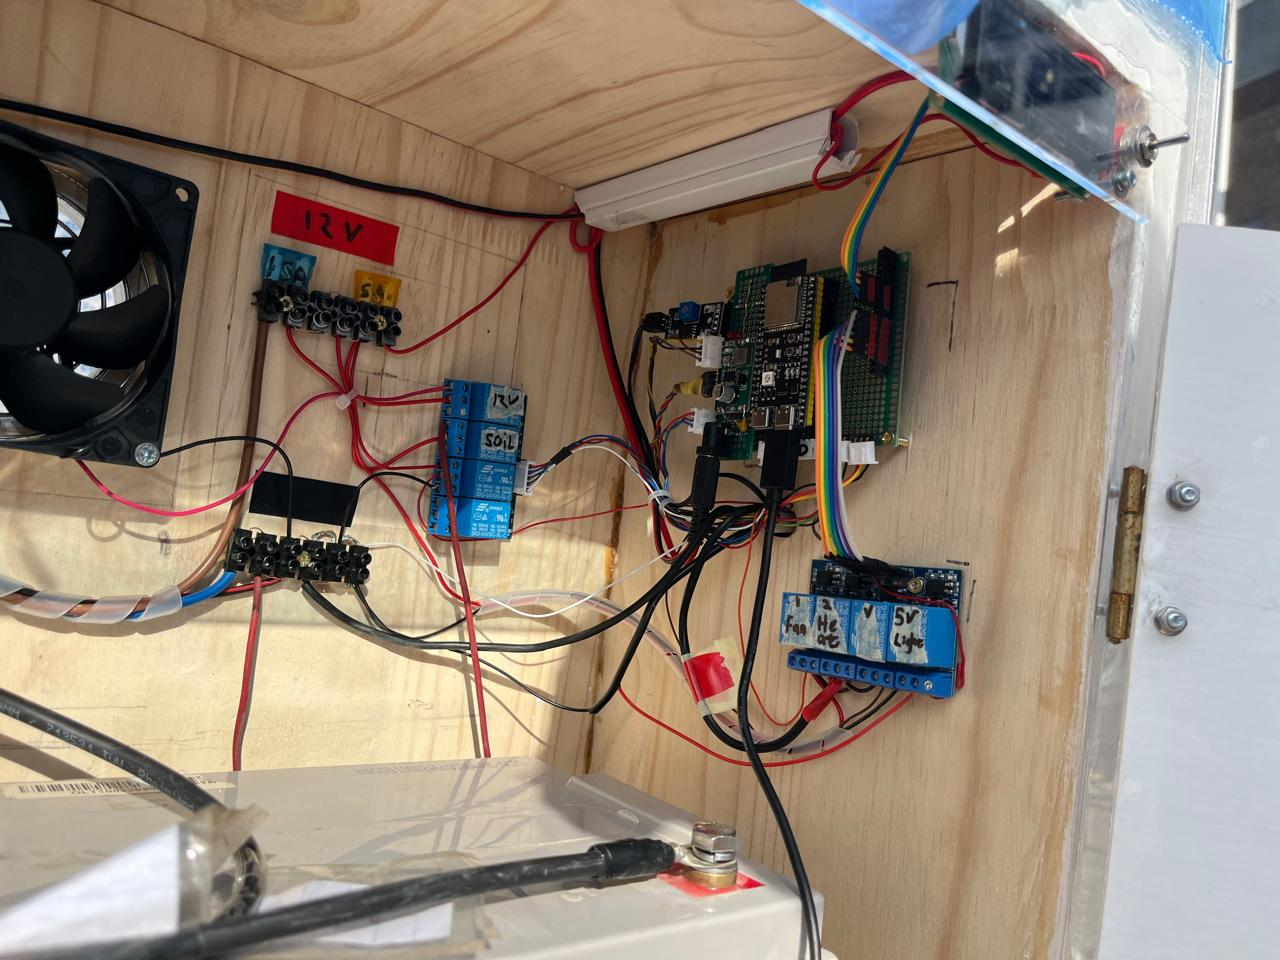
\includegraphics[width=\linewidth]{figs/room.jpeg}
		\caption{Control Room}
		\label{fig:Control Room}
	\end{subfigure}
	\begin{subfigure}[b]{0.25\linewidth}
		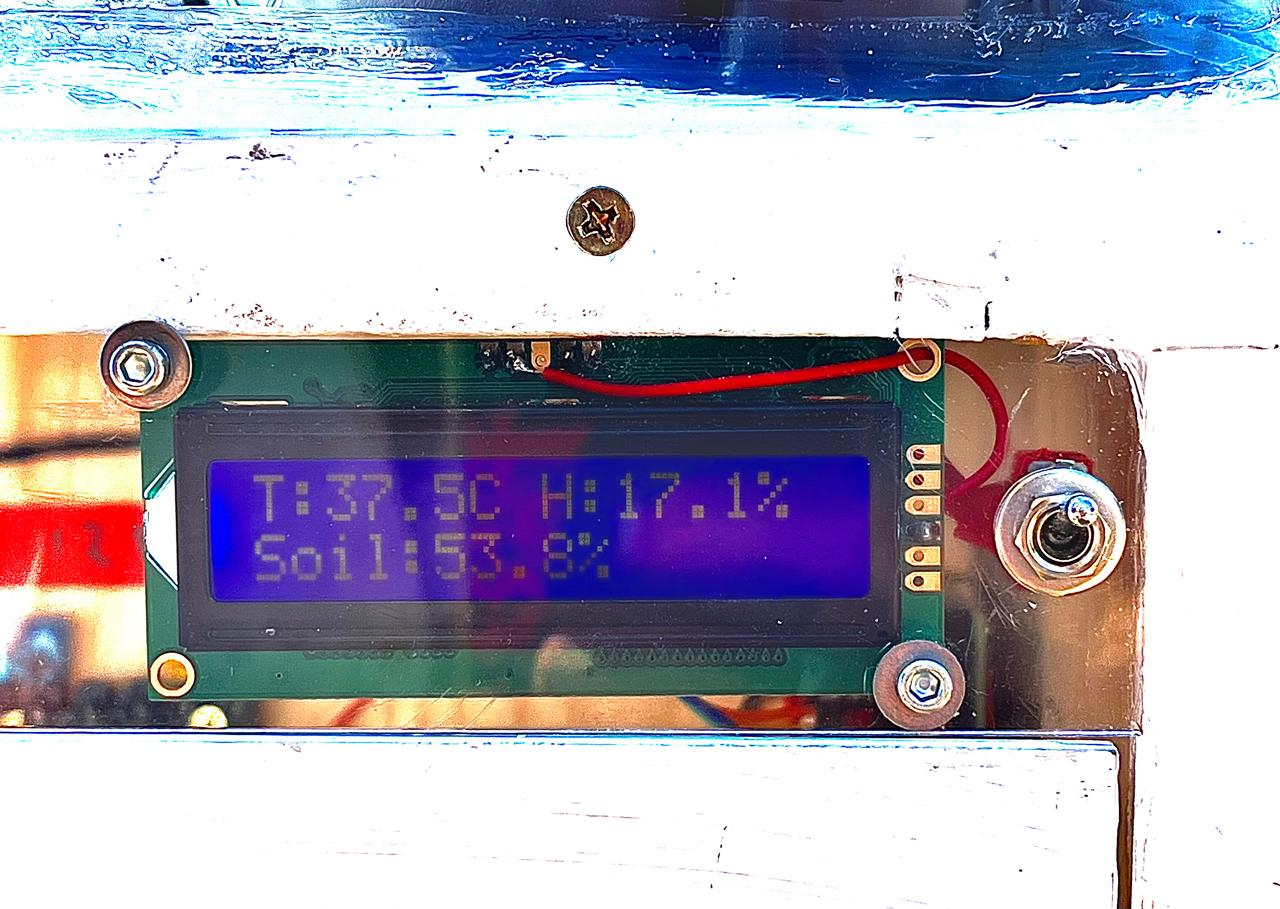
\includegraphics[width=\linewidth]{figs/LCD.jpeg}
		\caption{Local Monitoring}
		\label{fig:Local Monitoring}
	\end{subfigure}
	
	\caption{Overview of greenhouse hardware components and setup.}
	\label{fig:hardware_9}
\end{figure}


	\chapter{Responsible use of resources and an end-of-life strategy } 
The responsible use of resources and a well-defined end-of-life strategy are crucial to the project. Without a sustainable plan for decommissioning, the benefits of the project, such as advancing research in renewable energy and promoting food sustainability through small-scale greenhouses, could be overshadowed by the environmental impact of improperly discarded materials. 
During the design and construction phase of the project, opportunities to reuse previously used materials or use recycled material will be taken into consideration.
Once completed, the greenhouse can serve as a model to demonstrate the potential of engineering projects, inspire the adoption of renewable energy solutions, and promote education on food sustainability and self-sufficiency.
Once this post completion life cycle is over. The Project can be broken down and stripped of its parts. Some of the parts will go into storage to be reused for future engineering Thesis topics or other experiments to be used by the university at their own discretion. Other parts that are less likely to be reused are to be thrown out responsibly or recycled where possible. Special attention should be paid to proper disposal of hazardous materials.

\end{appendices}

\backmatter%----------------------------------------------------------
\bibliography{bib/GHreferences}
 
\end{document}   

